\documentclass{report}

\usepackage[utf8]{inputenc}
\usepackage[brazil]{babel}
%\usepackage{mathtools}
\usepackage{amssymb}
\usepackage{graphicx}
\graphicspath{{./Imagens/}}
\usepackage{subcaption}
\usepackage{epstopdf}
\usepackage{float}
\usepackage{listings}
\usepackage{courier}
\usepackage{eqnarray}
\usepackage{amsmath}
\usepackage[dvipsnames]{xcolor}
\usepackage{verbatim}

\lstset{
	backgroundcolor=\color[rgb]{1,1,0.9},
	frame = single,
	basicstyle = \footnotesize,
	keywordstyle = \color{blue},
	commentstyle = \color[rgb]{0,0.5,0},
	stringstyle = \color{Purple},
	showstringspaces = false,
	mathescape,
	breaklines = true,
	language = Matlab,
	inputencoding = utf8,
	extendedchars = true,
	literate = {ã}{{\~a}} 1
			   {é}{{\'e}} 1
			   {ç}{{\c{c}}} 1
			   {~}{{$\sim\ $}} 1
			   {ó}{{\'o}} 1
			   {á}{{\'a}} 1
			   {ú}{{\'u}} 1
}

\begin{document}

\begin{titlepage}
\begin{flushleft}

\textsc{\textbf{\LARGE Universidade Federal do Rio de Janeiro}}\\[0.5cm]
\textsc{\textbf{\LARGE COPPE}}\\[0.5cm]
\textsc{\textbf{\LARGE Programa de Engenharia Elétrica - PEE}}\\[0.5cm]
\textsc{\textbf{\LARGE Disciplina: Otimização Natural}}\\[0.5cm]
\textsc{\textbf{\LARGE Aluno: Gustavo Martins da Silva Nunes}}\\[0.5cm]
\textsc{\textbf{\LARGE Professor: José Gabriel}}\\[0.5cm]
\textsc{\textbf{\LARGE Data: 15/03/2016}}\\[6.5cm]

\end{flushleft}
\begin{center}
\textsc{\textbf{\huge Lista 1 - Resolução}}
\vfill
\end{center}
\end{titlepage}

\section*{Questão 1}

\textbf{Considere um processo de Markov $X(t)$ que tem três estados possíveis: 0, 1 e 2. A evolução deste processo é dada pela matriz de transição a seguir:}\\

\begin{equation*}
\mathbf{M} = \left[ \begin{array}{ccc}
0.50 & 0.25 & 0.25 \\ 
0.25 & 0.50 & 0.25 \\ 
0.25 & 0.25 & 0.50 
\end{array} \right]
\end{equation*}\\

\textbf{a) Considerando que a distribuição de probabilidade de $X(0)$ é dada pelo vetor $\mathbf{p}_0 = [0.3 \quad 0.4 \quad 0.3]^T$, calcule a distribuição de probabilidade de $X(3)$ (ou seja, do processo de Markov no instante $t = 3$).}\\

\paragraph{} A distribuição de probabilidade dos estados em cada instante $t$ é dada por:\\

\begin{equation}\label{eq:estados}
\mathbf{p}_t = \mathbf{M} \times \mathbf{p}_{t-1}, \quad t = 1, 2, ...
\end{equation}\\

\paragraph{} Seguindo a Equação \eqref{eq:estados}, temos, para $t = 1$:\\

\begin{equation*}
\mathbf{p}_1 = \mathbf{M} \times \mathbf{p}_0 = \left[ \begin{array}{ccc}
0.50 & 0.25 & 0.25 \\ 
0.25 & 0.50 & 0.25 \\ 
0.25 & 0.25 & 0.50 
\end{array} \right] \times \left[\begin{array}{c}
0.3 \\ 
0.4 \\ 
0.3
\end{array} \right] = \left[ \begin{array}{c}
0.3250 \\ 
0.3500 \\ 
0.3250
\end{array}  \right]
\end{equation*}\\

\paragraph{} Da mesma forma, calcula-se o vetor $\mathbf{p}_2$, substituindo, somente, o estado inicial $\mathbf{p}_0$ por $\mathbf{p}_1$:\\

\begin{equation*}
\mathbf{p}_1 = \mathbf{M} \times \mathbf{p}_0 = \left[ \begin{array}{ccc}
0.50 & 0.25 & 0.25 \\ 
0.25 & 0.50 & 0.25 \\ 
0.25 & 0.25 & 0.50 
\end{array} \right] \times \left[\begin{array}{c}
0.3250, \\ 
0.3500 \\ 
0.3250
\end{array} \right] = \left[ \begin{array}{c}
0.3312 \\ 
0.3375 \\ 
0.3313
\end{array}  \right]
\end{equation*}\\

\paragraph{} Finalmente, em $t = 3$:\\

\begin{equation*}
\mathbf{p}_1 = \mathbf{M} \times \mathbf{p}_0 = \left[ \begin{array}{ccc}
0.50 & 0.25 & 0.25 \\ 
0.25 & 0.50 & 0.25 \\ 
0.25 & 0.25 & 0.50 
\end{array} \right] \times \left[\begin{array}{c}
0.3312, \\ 
0.3375 \\ 
0.3313
\end{array} \right] = \left[ \begin{array}{c}
0.3328 \\ 
0.3344 \\ 
0.3328
\end{array}  \right]
\end{equation*}\\

\paragraph{} O código, em MATLAB, que implementa a solução deste item encontra-se abaixo:\\

\begin{lstlisting}

M = [0.50 0.25 0.25; 0.25 0.50 0.25; 0.25 0.25 0.50];
p0 = [0.3 0.4 0.3]';

p = p0;

for i = 1:3
    p = M * p;
end

p

% Resultado:
%
% p =
%
%    0.3328
%    0.3344
%    0.3328

\end{lstlisting}

\textbf{b) Iniciando em $X(0) = 1$ e usando um gerador de números aleatórios (são necessários apenas três números aleatórios equiprováveis), calcule manualmente uma amostra do processo $X(t)$ até $t = 3$.}\\

\paragraph{} Dado que o estado inicial é 1, temos que o vetor de distribuição de probabilidades inicial $\mathbf{p}_0 = [0 \quad 1 \quad 0]^T$. Aplicando esse vetor na Equação \eqref{eq:estados}, encontra-se $\mathbf{p}_1$.\\

\begin{equation*}
\mathbf{p}_1 = \mathbf{M} \times \mathbf{p}_0 = \left[ \begin{array}{ccc}
0.50 & 0.25 & 0.25 \\ 
0.25 & 0.50 & 0.25 \\ 
0.25 & 0.25 & 0.50 
\end{array} \right] \times \left[\begin{array}{c}
0 \\ 
1 \\ 
0
\end{array} \right] = \left[ \begin{array}{c}
0.25 \\ 
0.50 \\ 
0.25
\end{array}  \right]
\end{equation*}\\

\paragraph{} Com isso, as amostras do processo $X(t)$, no instante $t = 1$ seguem a distribuição de probabilidade dada por $\mathbf{p}_1$. A PDF e a CDF dessa distribuição estão exibidas na Figura \ref{pdf_cdf_p1}.\\

\begin{figure}[H]
	\centering
	\begin{subfigure}{0.4\textwidth}
		\centering
		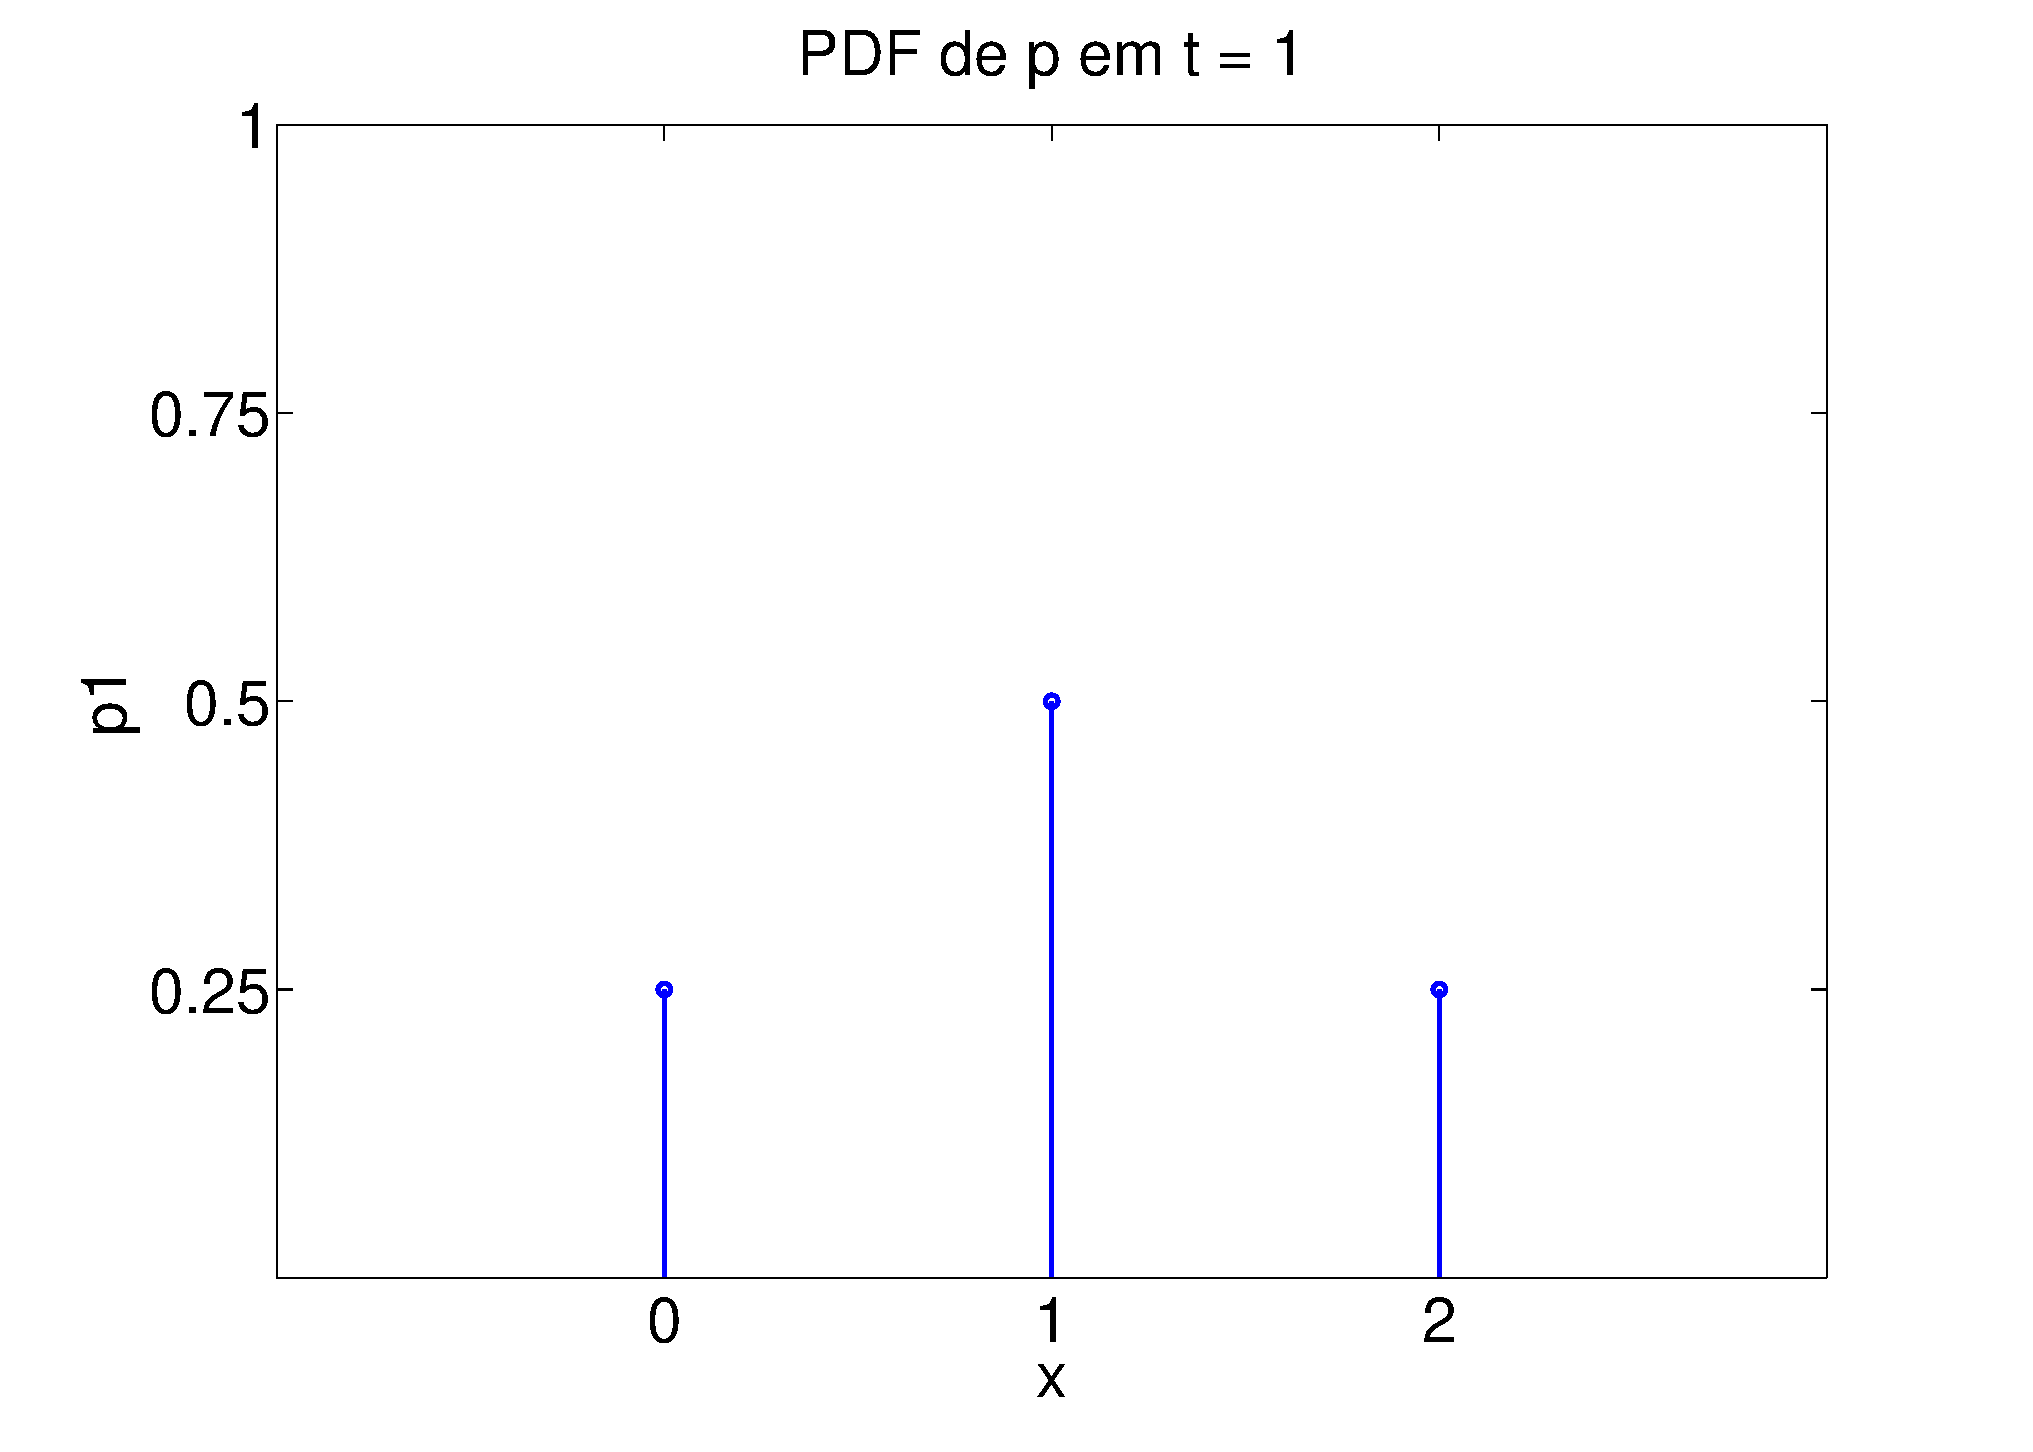
\includegraphics[width = \textwidth]{Q1_b_pdf_p1}
		\caption{PDF de $\mathbf{p}_1$}
		\label{pdf_p1}
	\end{subfigure}
	\begin{subfigure}{0.4\textwidth}
		\centering
		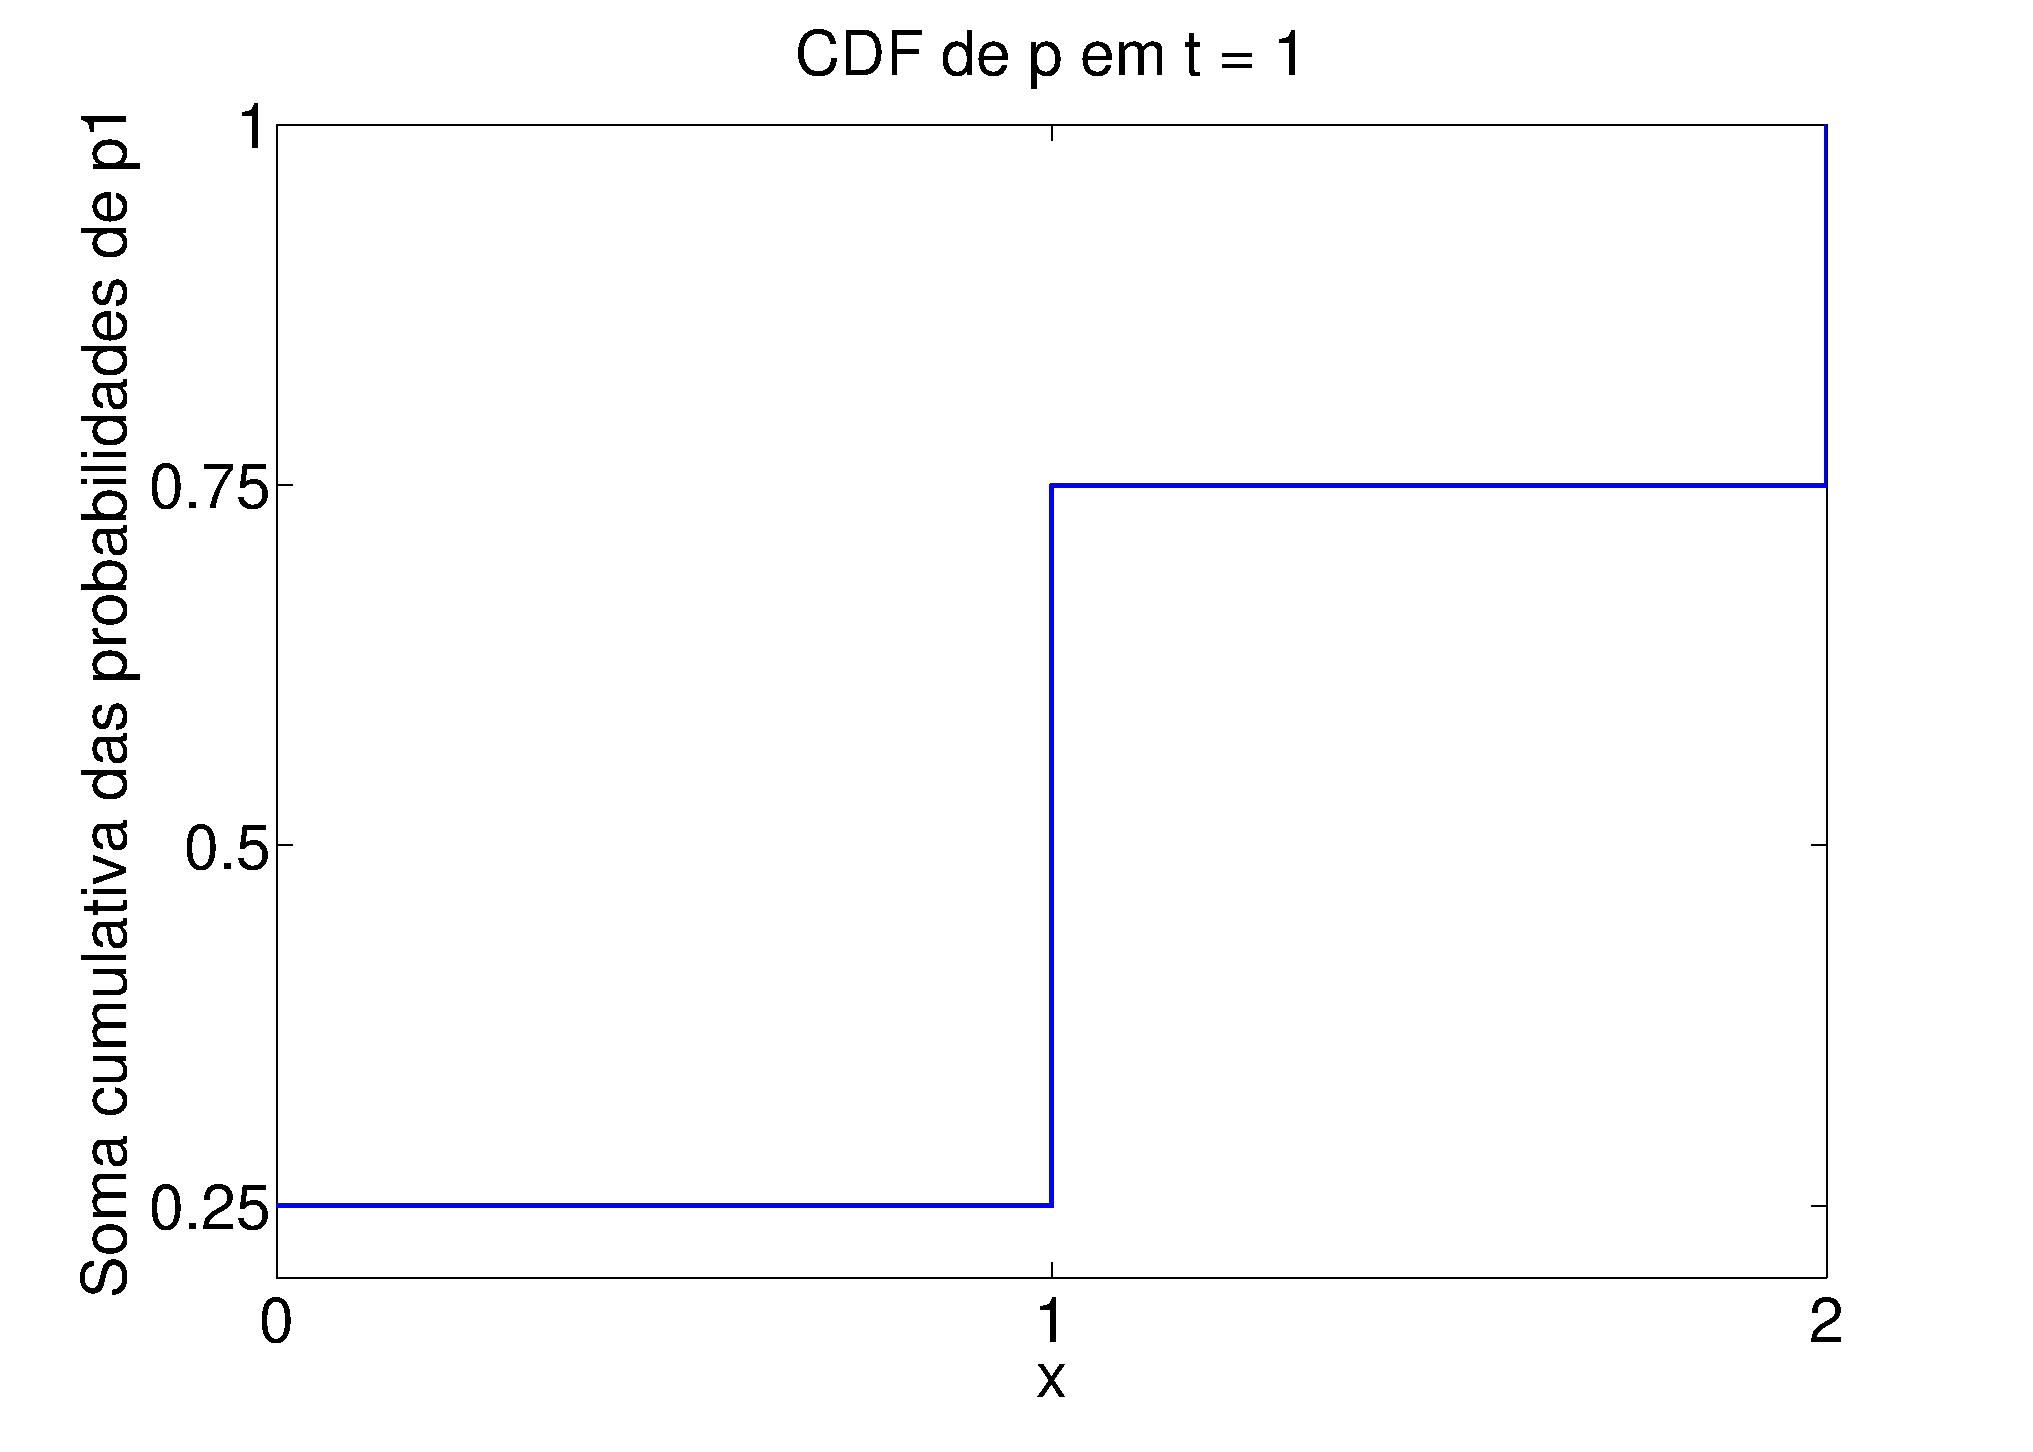
\includegraphics[width = \textwidth]{Q1_b_cdf_p1}
		\caption{CDF de $\mathbf{p}_1$}
		\label{cdf_p1}
	\end{subfigure}
	\caption{Informações sobre a distribuição de probabilidade $\mathbf{p}_1$}
	\label{pdf_cdf_p1}
\end{figure}

\paragraph{} Observando a CDF na Figura \ref{cdf_p1}, conclui-se que $P(X(1) \leq 0) = P(X(1) = 0) = 0,25$, $P((X(1) \leq 1) \cap (X(1) > 0)) = P(X(1) = 1) = 0,50$ e $P(X(1) > 1) = P(X(1) = 2) = 0,25$. Sendo assim, sorteando-se um número aleatório da distribuição uniforme entre [0, 1] e mapeando esse número em um estado segundo a CDF apresentada, obtém-se um estado $X(1)$ segundo a distribuição de probabilidade dada por $\mathbf{p}_1$.\\

\begin{equation*}
X(1) =  \begin{cases}
			0, \quad	r \leq 0.25\\
			1, \quad	0 < r \leq 0.75\\
			2, \quad	r > 0.75
		\end{cases} , \quad r \in (0,1)
\end{equation*}\\

\paragraph{} Sorteando, então, $r = 0,1$, chega-se a $X(1) = 0$. O mesmo procedimento é adotado para as iterações subsequentes, calculando-se a nova distribuição $\mathbf{p}$ e sorteando uma amostra segundo essa distribuição, usando a mesma abordagem (alterando, somente, os intervalos de $r$ que mapeiam o estado, de forma a respeitar a distribuição em questão).\\

\begin{equation*}
\mathbf{p}_2 = \mathbf{M} \times \mathbf{p}_1 = \left[ \begin{array}{ccc}
0.50 & 0.25 & 0.25 \\ 
0.25 & 0.50 & 0.25 \\ 
0.25 & 0.25 & 0.50 
\end{array} \right] \times \left[\begin{array}{c}
0.25 \\ 
0.50 \\ 
0.25
\end{array} \right] = \left[ \begin{array}{c}
0.3125 \\ 
0.3750 \\ 
0.3125
\end{array}  \right]
\end{equation*}\\

\paragraph{} Sorteando $r = 0,2$, temos que $X(2) = 0$. Executando a última iteração:\\

\begin{equation*}
\mathbf{p}_2 = \mathbf{M} \times \mathbf{p}_1 = \left[ \begin{array}{ccc}
0.50 & 0.25 & 0.25 \\ 
0.25 & 0.50 & 0.25 \\ 
0.25 & 0.25 & 0.50 
\end{array} \right] \times \left[\begin{array}{c}
0.3125 \\ 
0.3750 \\ 
0.3125
\end{array} \right] = \left[ \begin{array}{c}
0.3281 \\ 
0.3438 \\ 
0.3281
\end{array}  \right]
\end{equation*}\\

\paragraph{} Sorteando $r = 0,8$, temos que $X(3) = 2$. Com isso, os estados sorteados em cada um dos 4 instantes foram: $\mathbf{x} = [X(0) \quad X(1) \quad X(2) \quad X(3)] = [1 \quad 0 \quad 0 \quad 2]$.\\ 

\textbf{c) Usando um computador, execute 100 repetições do item (b). Em cada uma das 100 repetições, comece a simulação com um valor diferente de $X(0)$, assumindo que os eventos $X(0) = 0$, $X(0) = 1$ e $X(0) = 2$ são equiprováveis. Armazene as 100 cadeias obtidas em uma matriz $\mathbf{X}$, com 4 colunas ($t = 0$ até $t = 3$) e 100 linhas.}\\

\paragraph{} O código, em MATLAB, que implementa a solução deste item é apresentado a seguir:\\

\begin{lstlisting}
N = 100;
T = 4;

X = zeros(N,T);
M = [0.50 0.25 0.25; 0.25 0.50 0.25; 0.25 0.25 0.50];
p0 = [0.33 0.33 0.33]';

for n = 1:100 
    
    p = p0;

    for i = 0:(T-1)
        
        if (i ~= 0) % Não é o estado inicial
            p = M * p;
            r = rand();

            p_cdf = cumsum(p); % CDF da distribuição p

            for j = 1:length(p_cdf)
                if r <= p_cdf(j)
                    switch j
                        case 1 
                            x = 0;
                        case 2
                            x = 1;
                        case 3
                            x = 2;
                    end
                break;
                end
            end
            
            X(n, i+1) = x;
            
        else % Estado inicial; apenas inicializa X(n, 1)
            X(n, i+1) = random('unid', 3) - 1; % Estado Inicial    
        end
    end
end

\end{lstlisting}

\textbf{d) Fazendo histogramas de cada uma das 4 colunas, calcule as distribuições de probabilidade do processo $X(t)$ em cada um dos 4 instantes: $t = 0, 1, 2, 3$. Comente os resultados obtidos.}

\paragraph{} Os histogramas dos estados em cada um dos 4 instantes encontram-se na Figura \ref{histogramas_estados}. Uma aproximação das distribuições representadas por cada histogramas estão exibidas na Figura \ref{pdfs_estados}.\\

\begin{figure}[H]
	\centering
	\begin{subfigure}{0.4\textwidth}
		\centering
		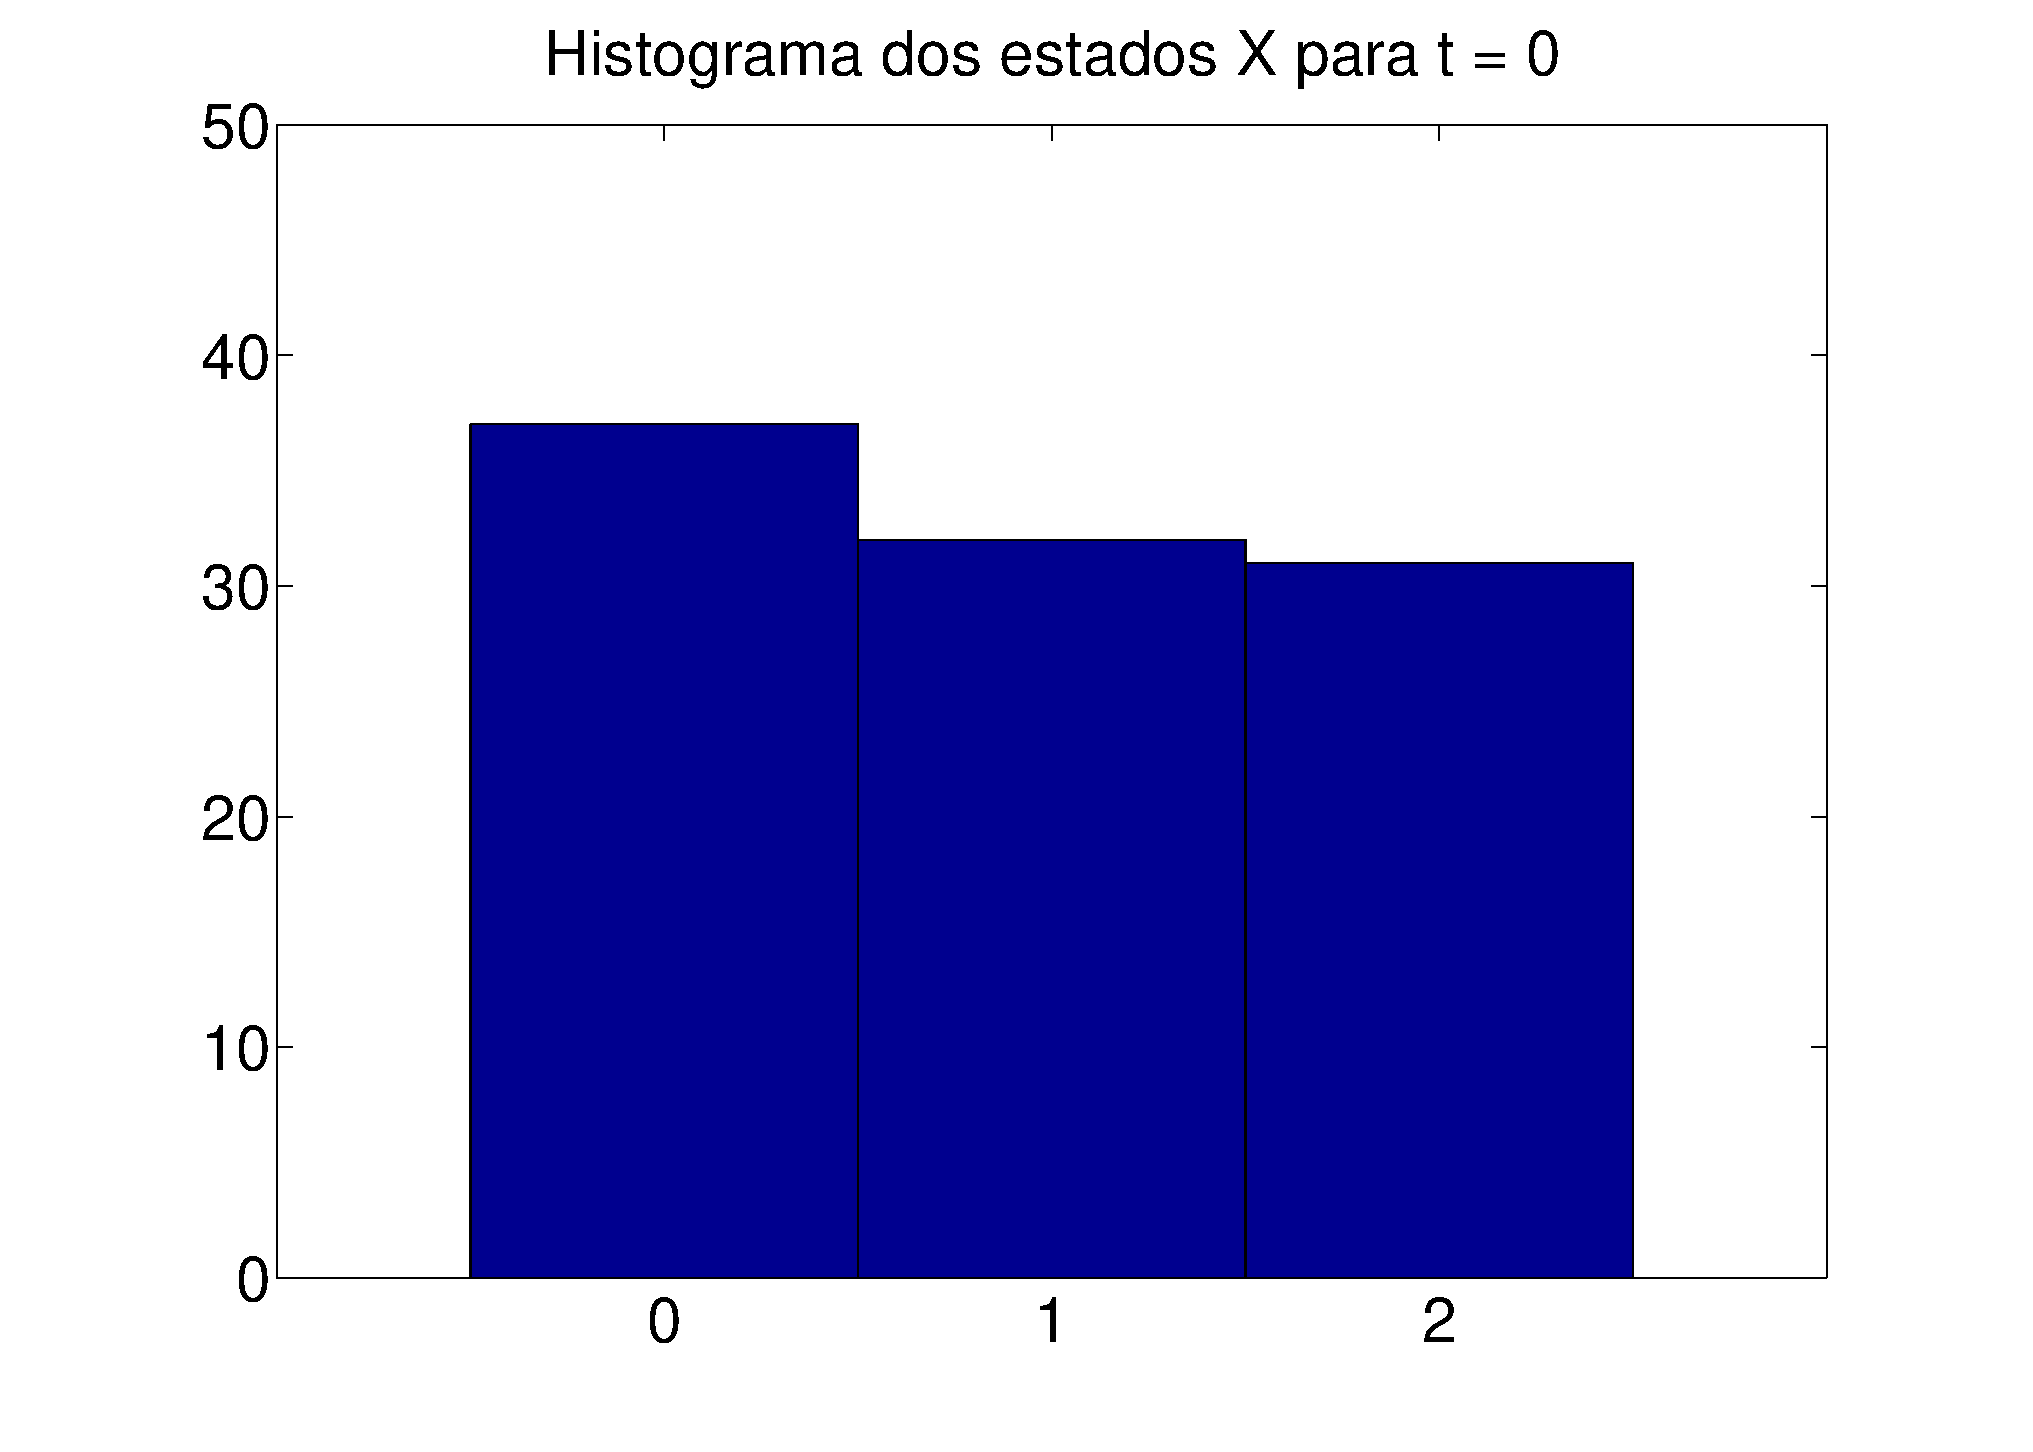
\includegraphics[width = \textwidth]{Q1_d_histograma_x_0}
		\caption{$t = 0$}
	\end{subfigure}
	\begin{subfigure}{0.4\textwidth}
		\centering
		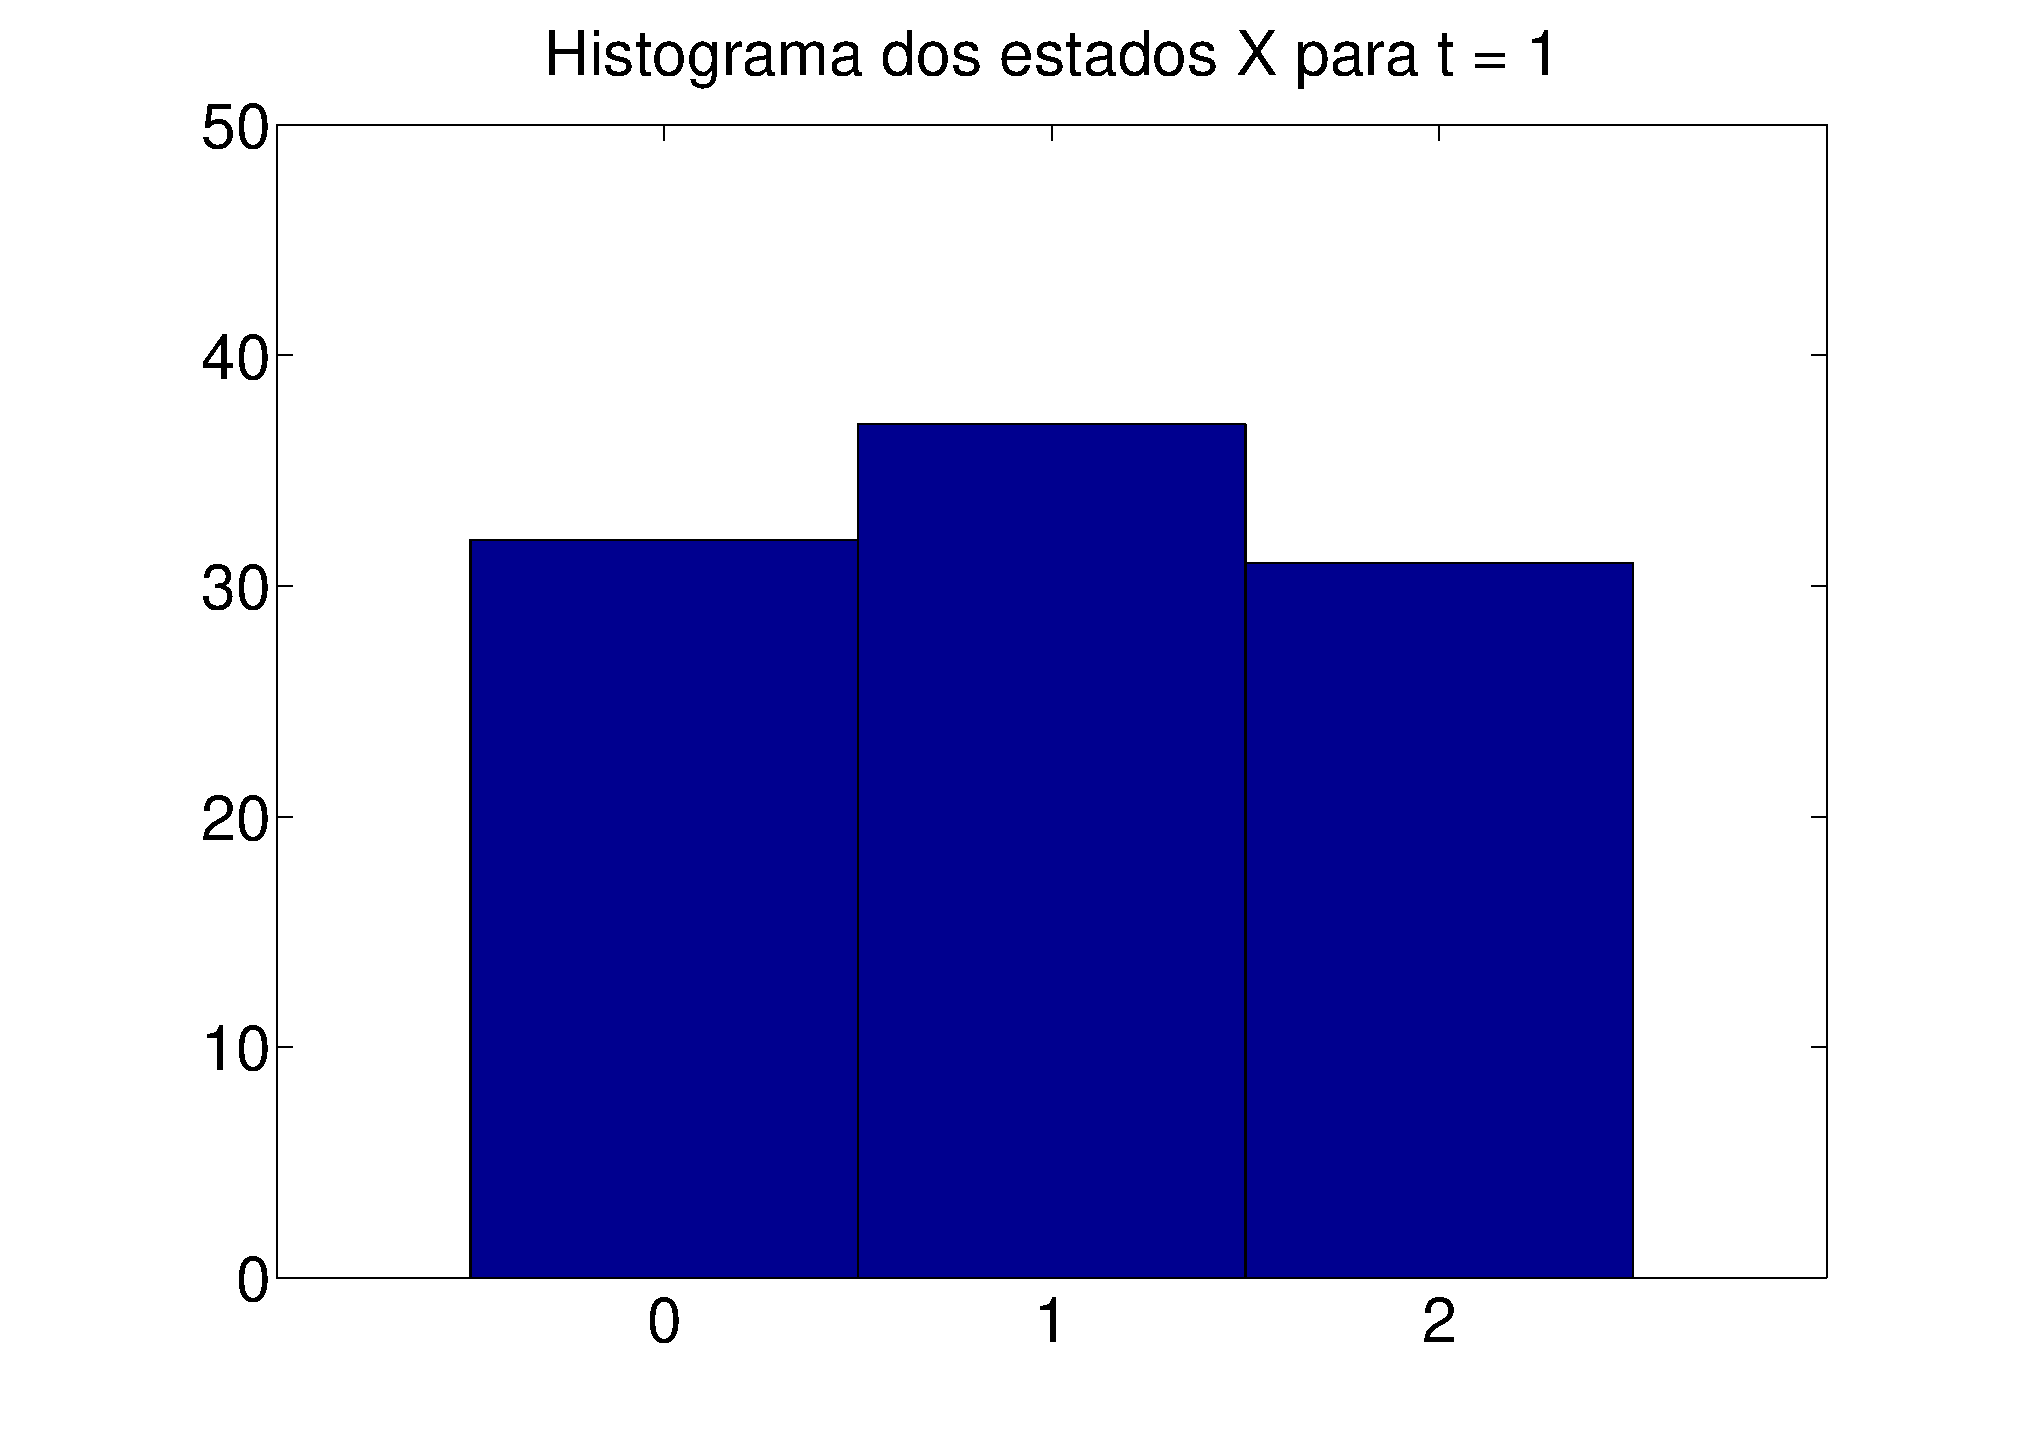
\includegraphics[width = \textwidth]{Q1_d_histograma_x_1}
		\caption{$t = 1$}
	\end{subfigure}
	\begin{subfigure}{0.4\textwidth}
		\centering
		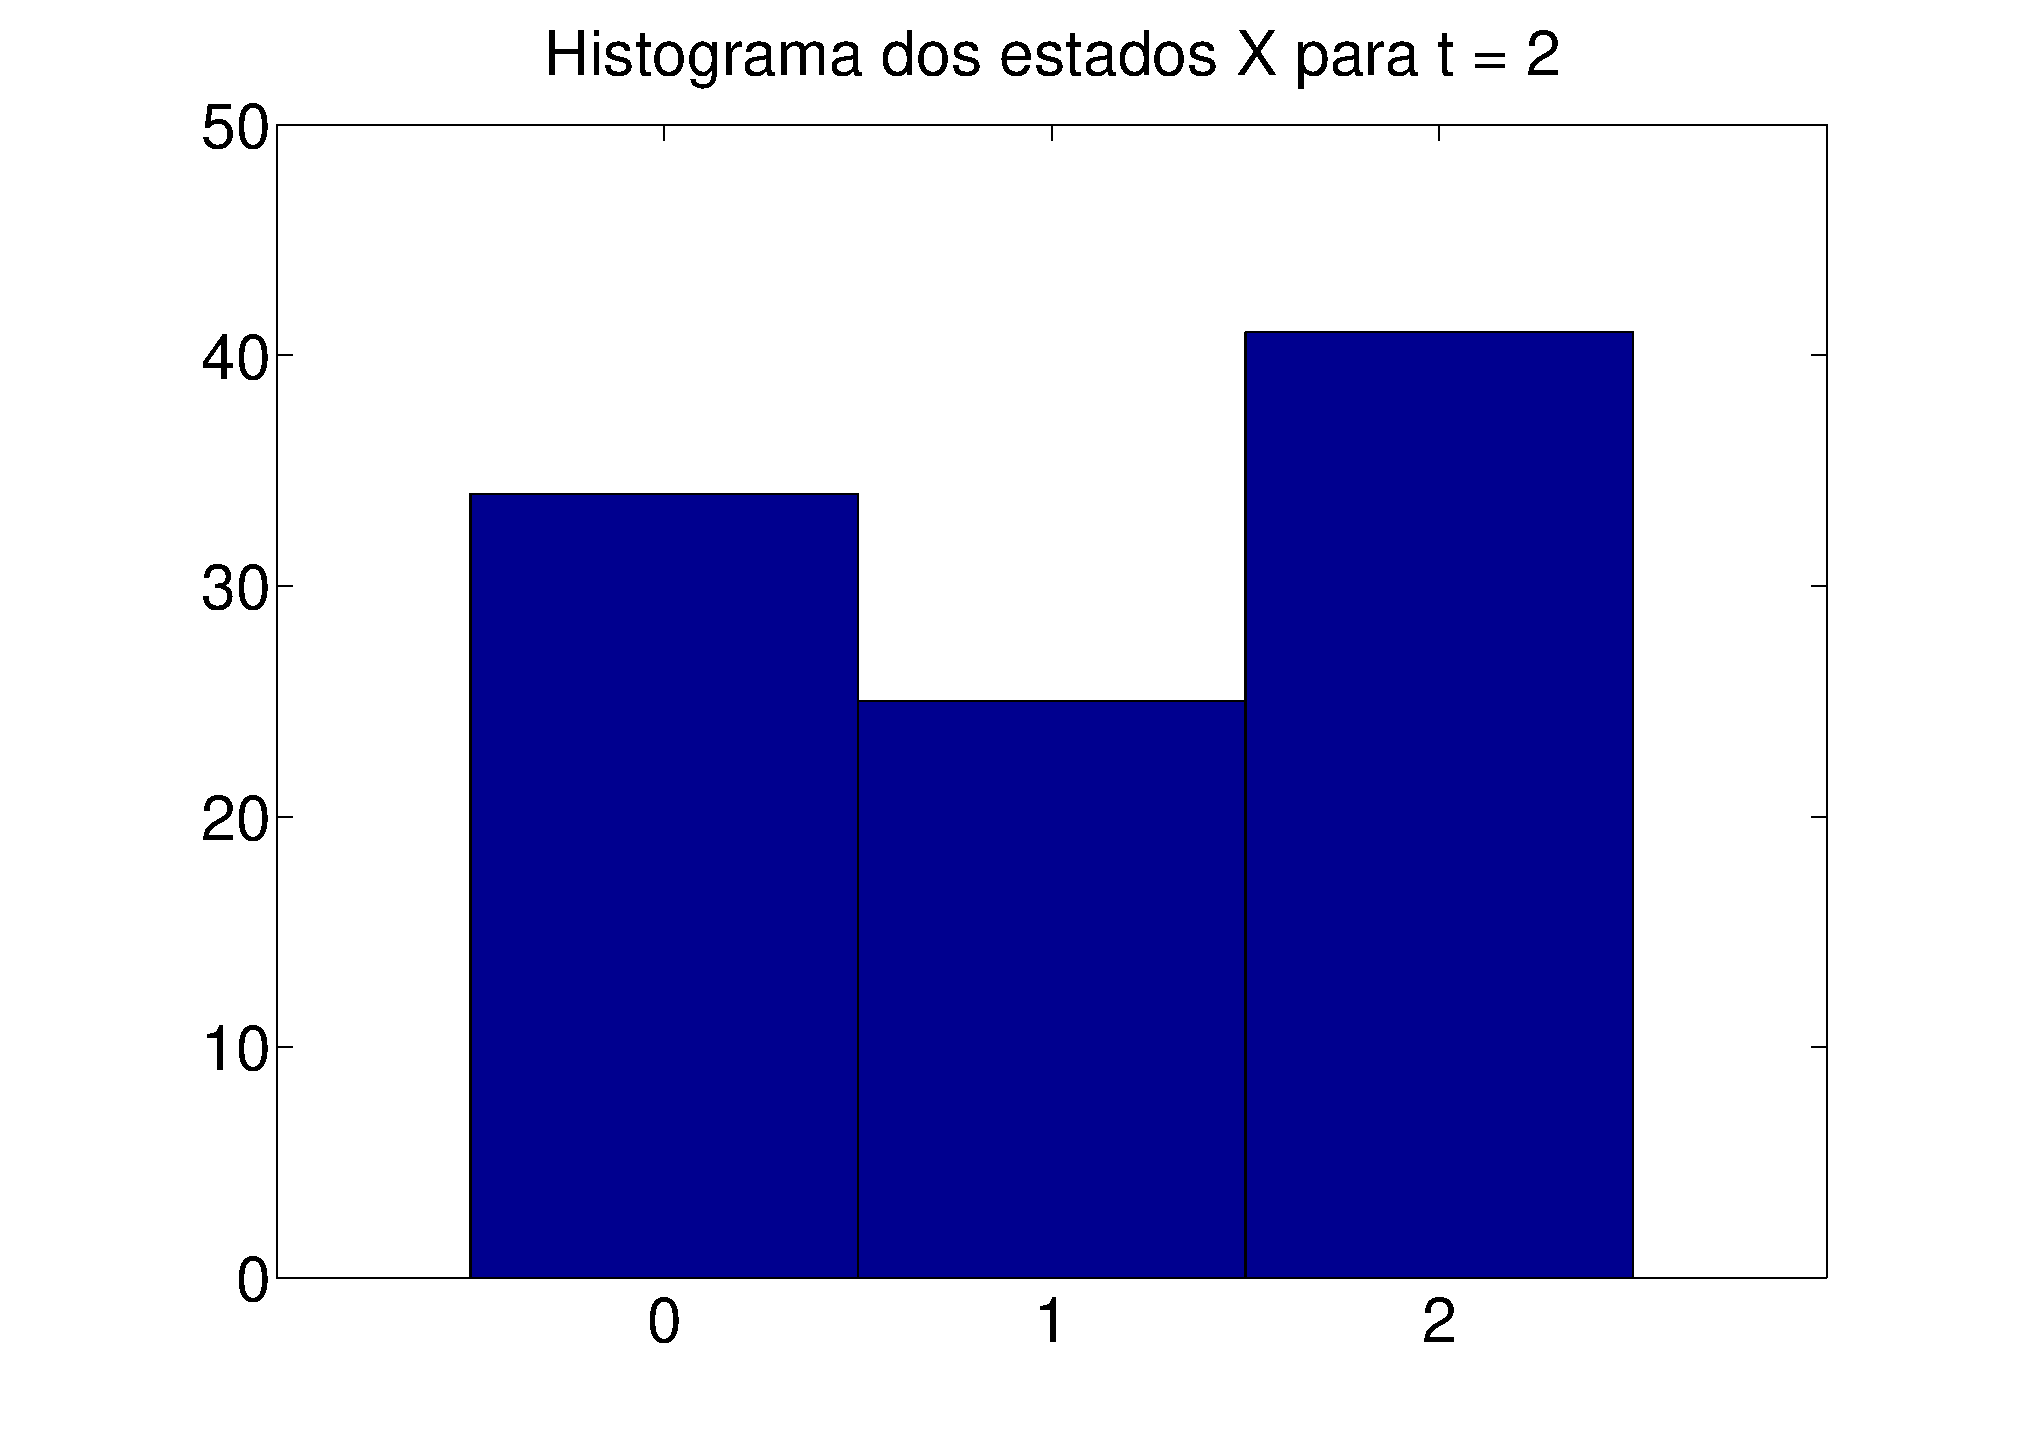
\includegraphics[width = \textwidth]{Q1_d_histograma_x_2}
		\caption{$t = 2$}
	\end{subfigure}
	\begin{subfigure}{0.4\textwidth}
		\centering
		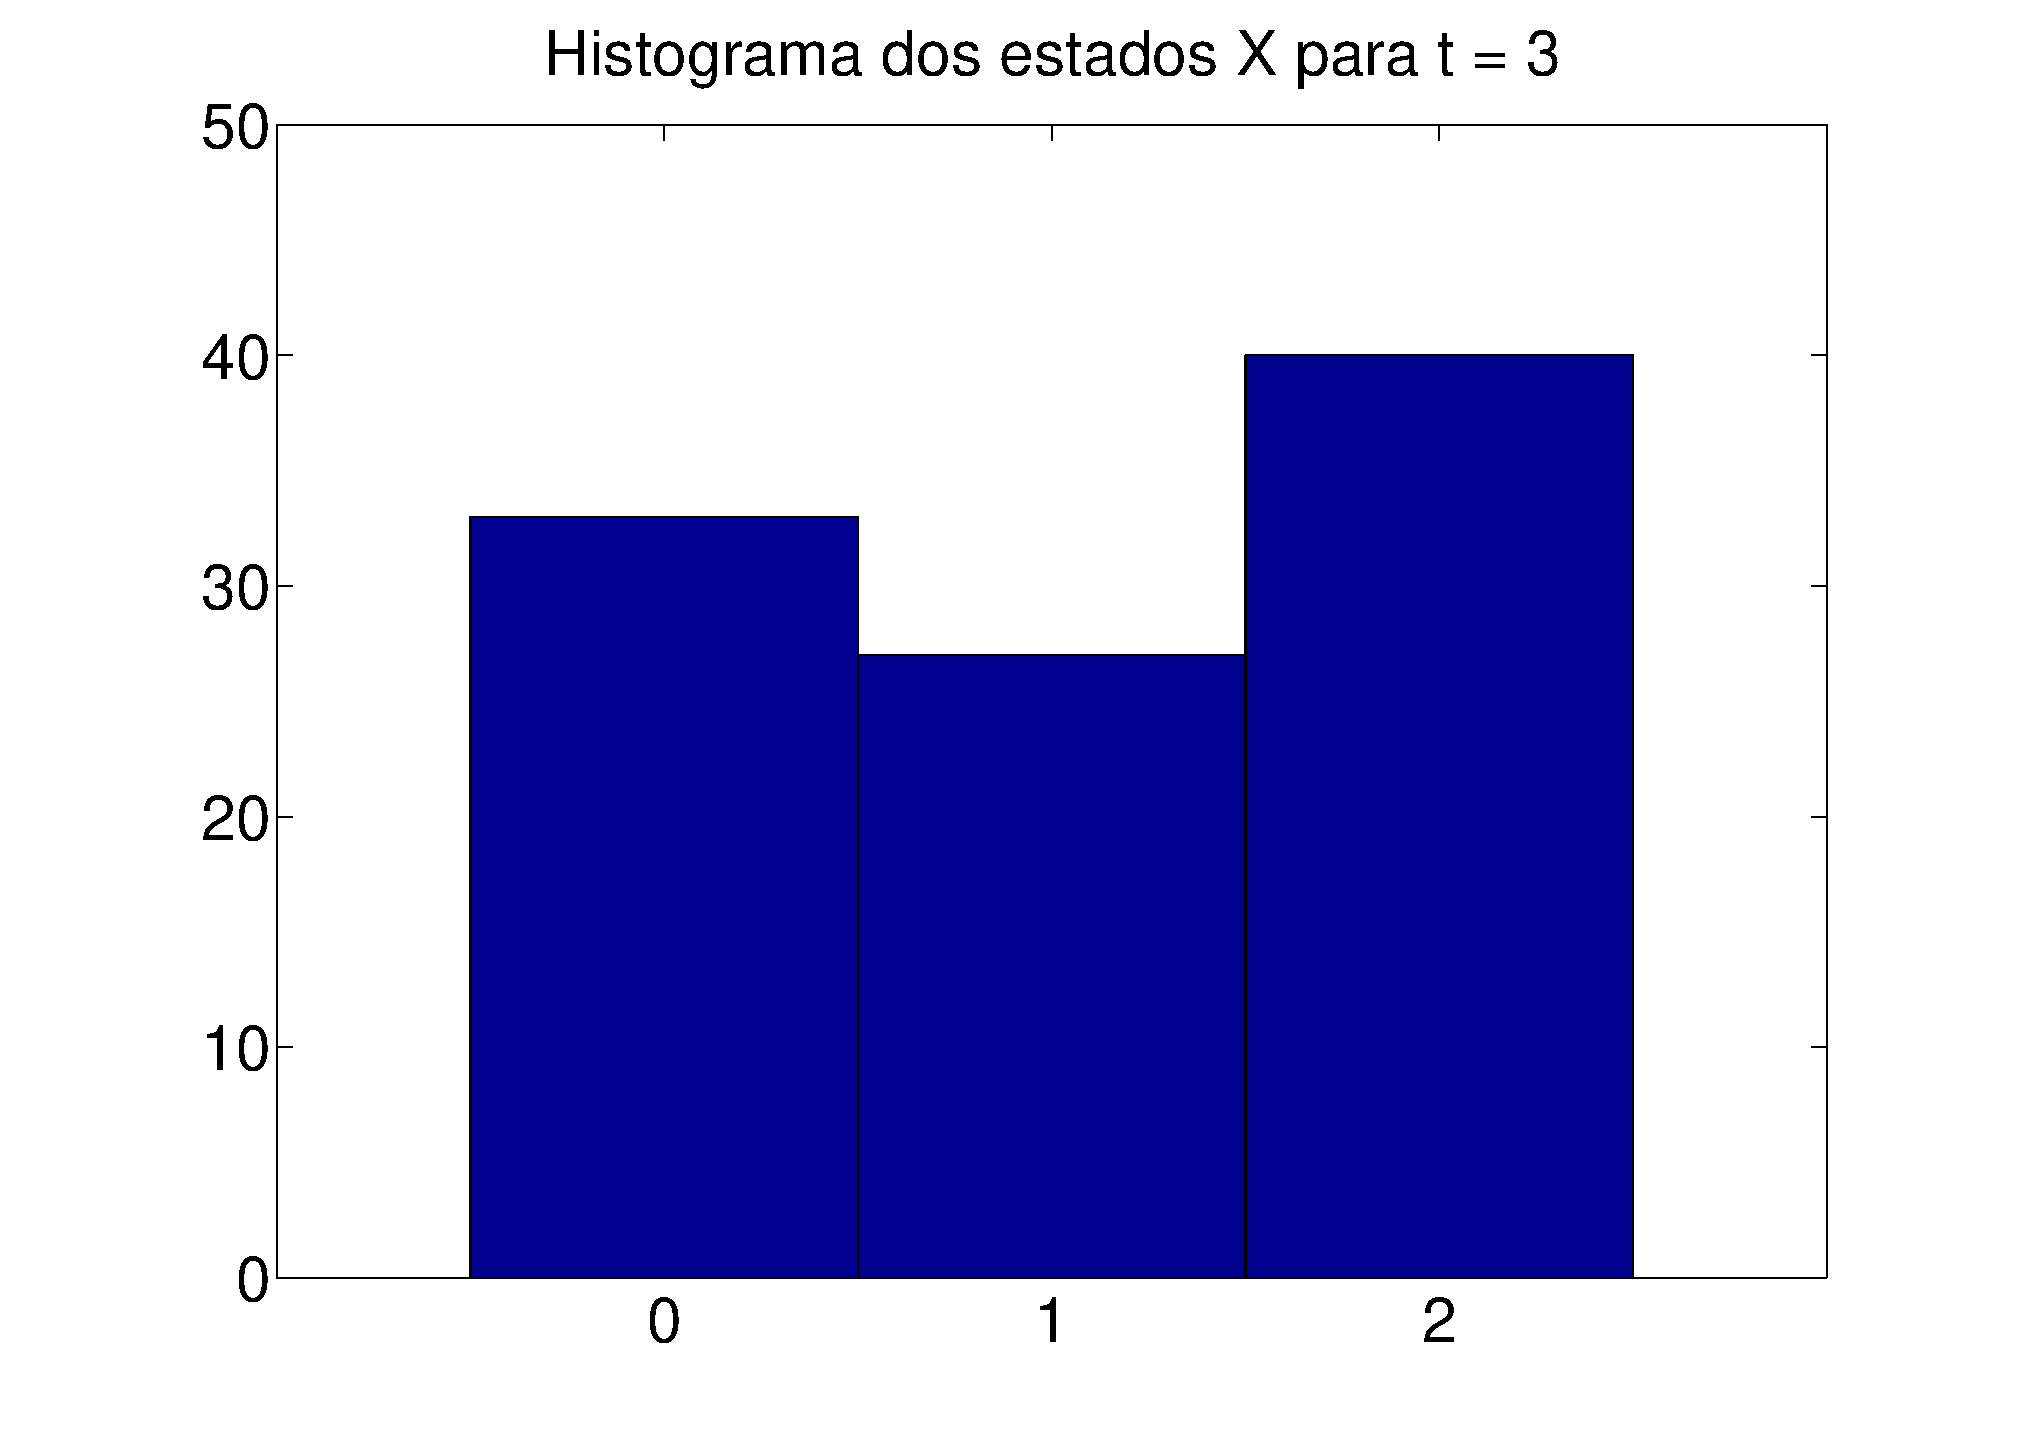
\includegraphics[width = \textwidth]{Q1_d_histograma_x_3}
		\caption{$t = 3$}
	\end{subfigure}
	\caption{Histogramas de $X(t)$}
	\label{histogramas_estados}
\end{figure}

\begin{figure}[H]
	\centering
	\begin{subfigure}{0.4\textwidth}
		\centering
		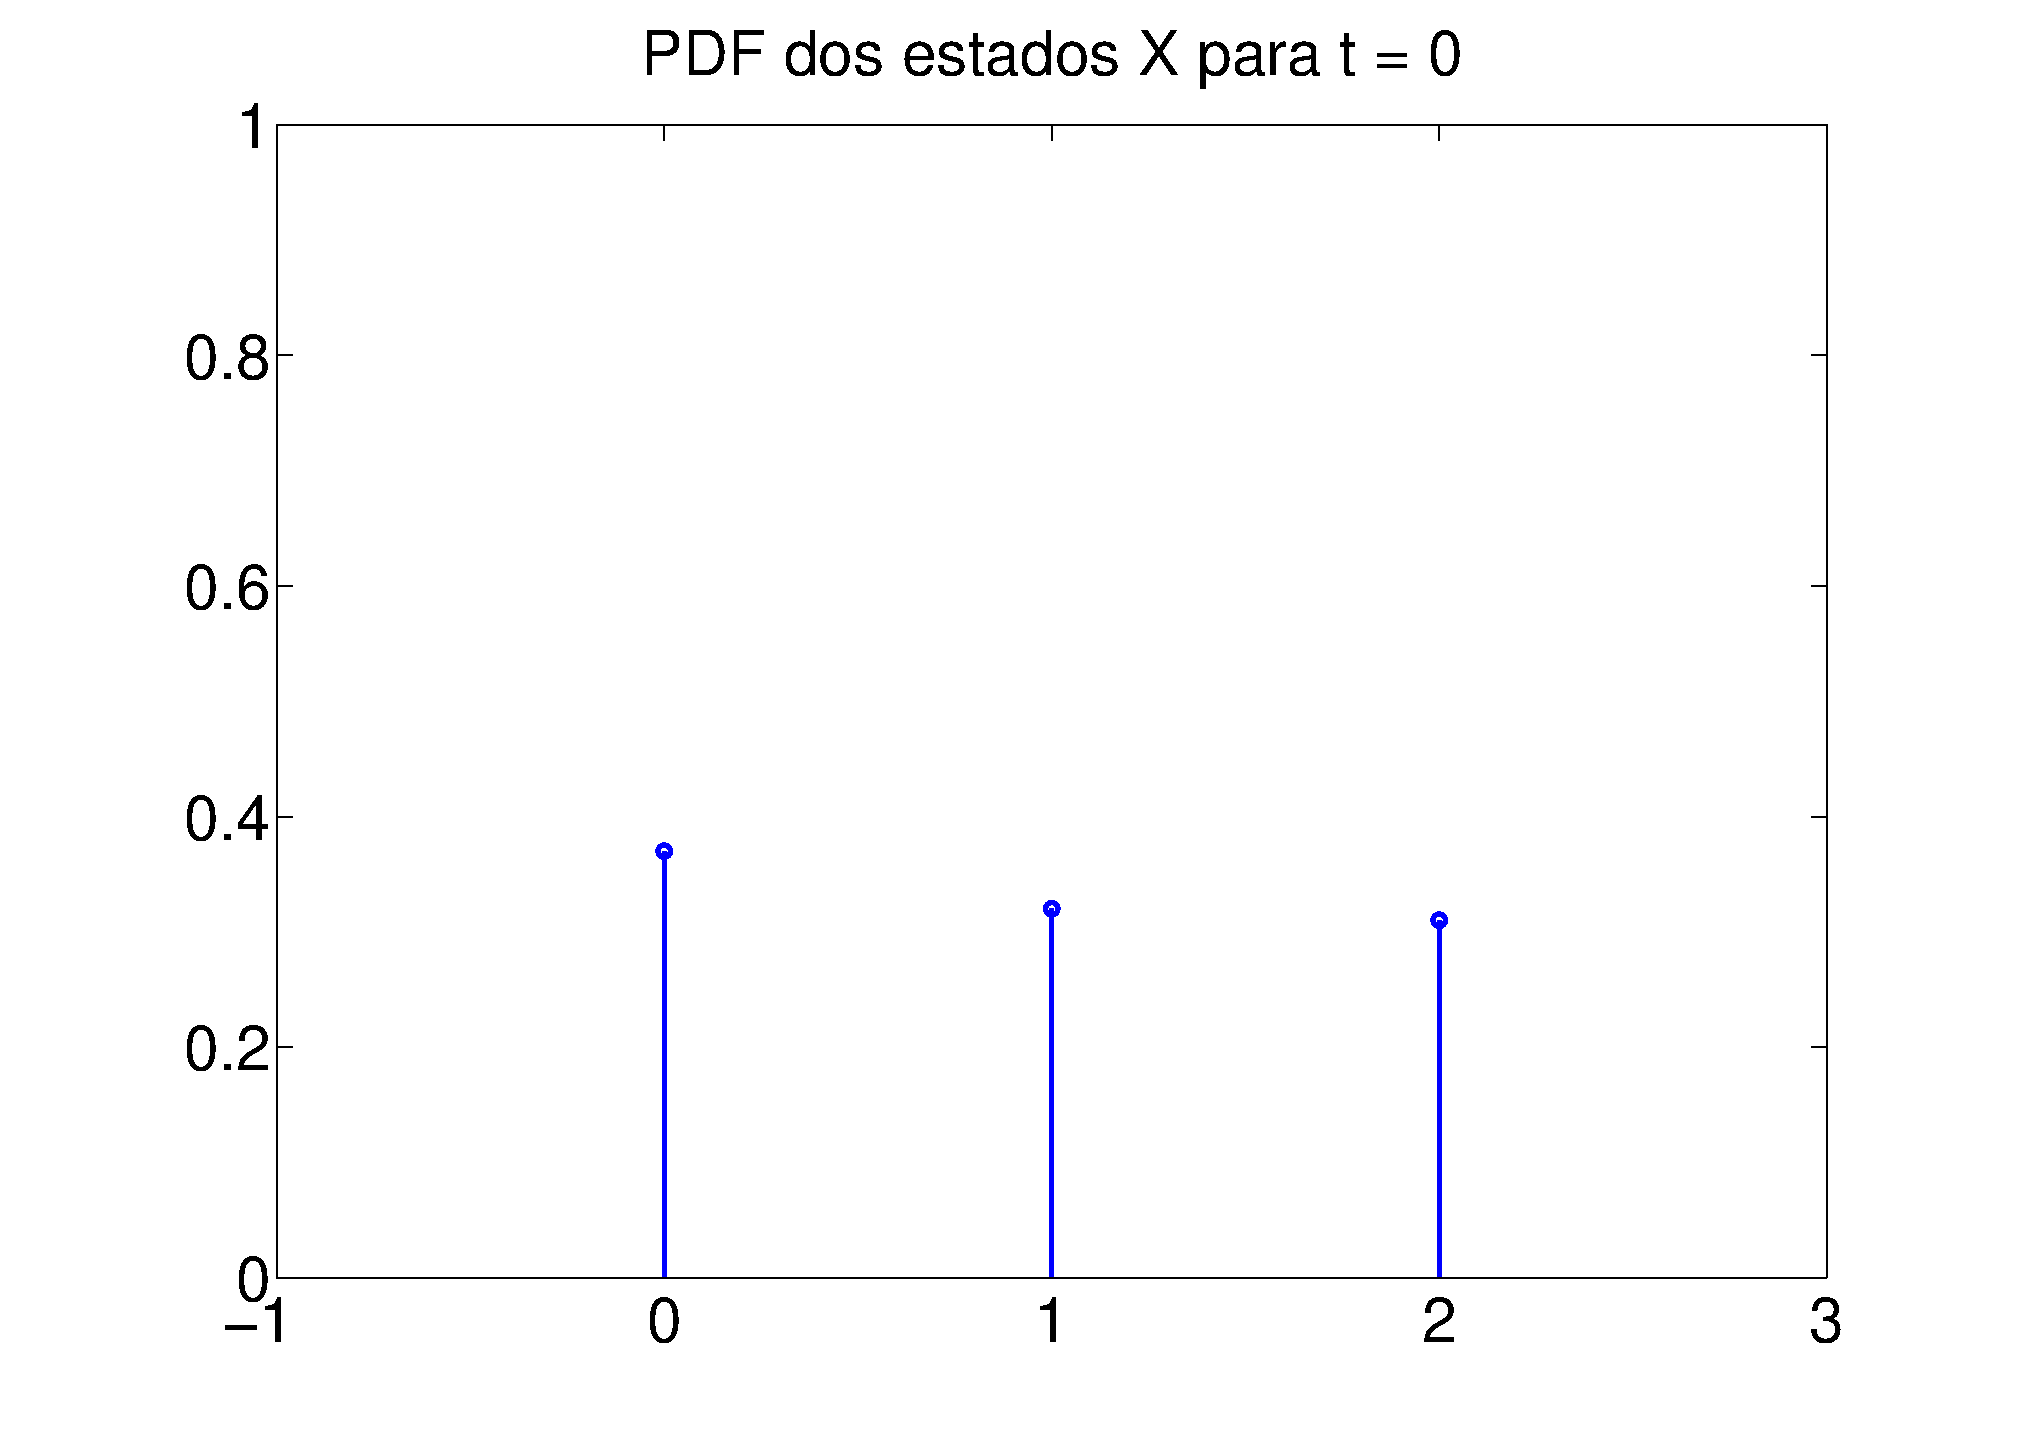
\includegraphics[width = \textwidth]{Q1_d_pdf_x_0}
		\caption{$t = 0$}
	\end{subfigure}
	\begin{subfigure}{0.4\textwidth}
		\centering
		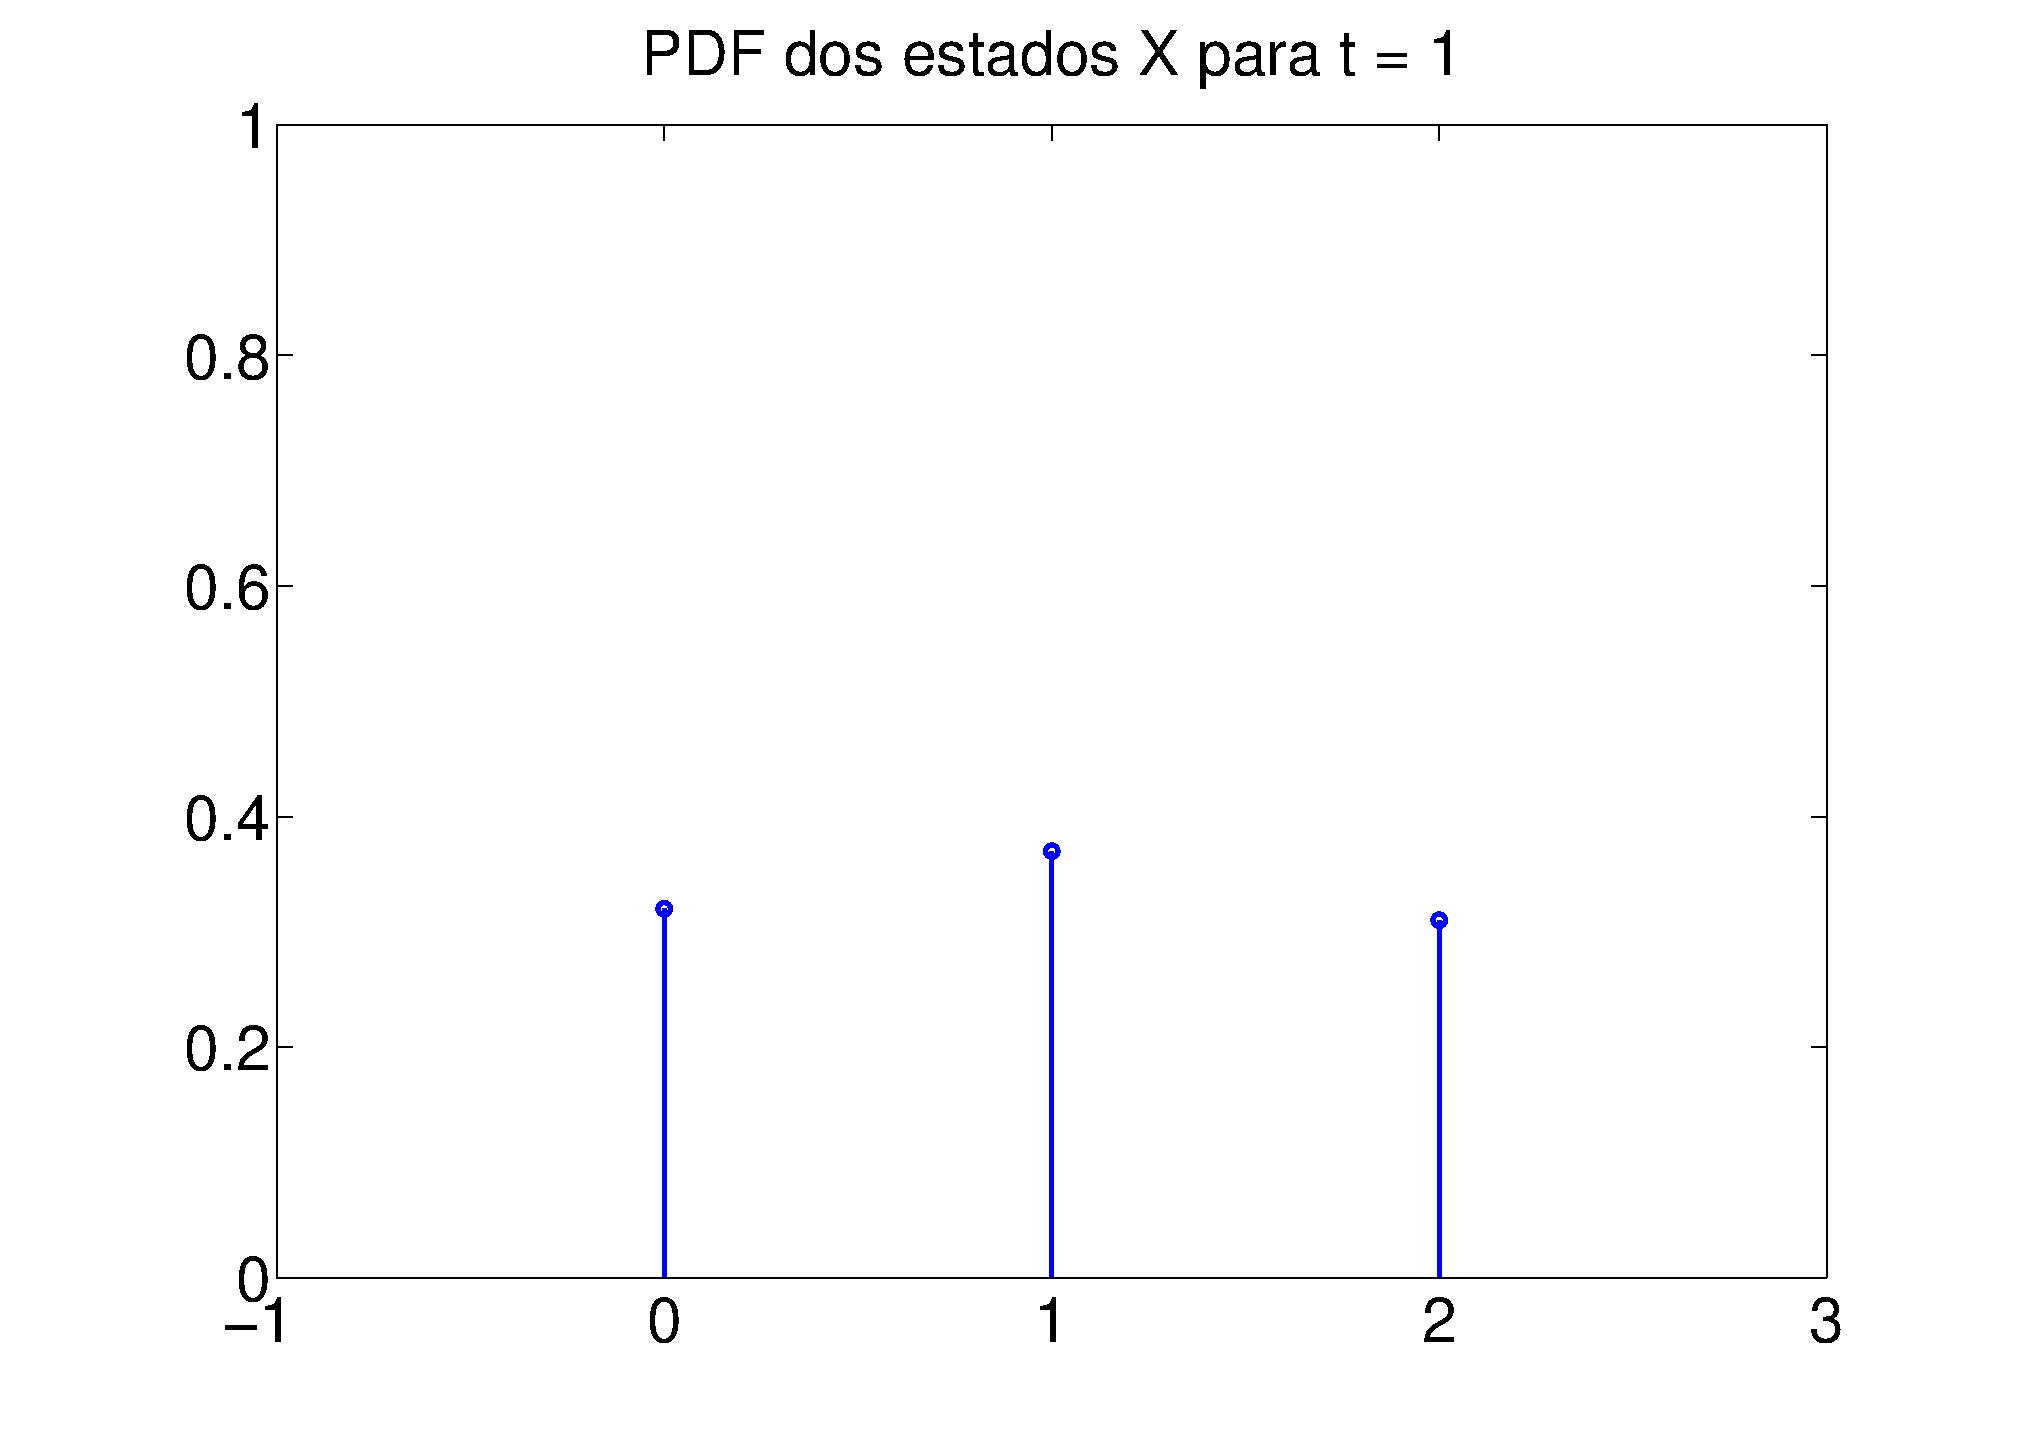
\includegraphics[width = \textwidth]{Q1_d_pdf_x_1}
		\caption{$t = 1$}
	\end{subfigure}
	\begin{subfigure}{0.4\textwidth}
		\centering
		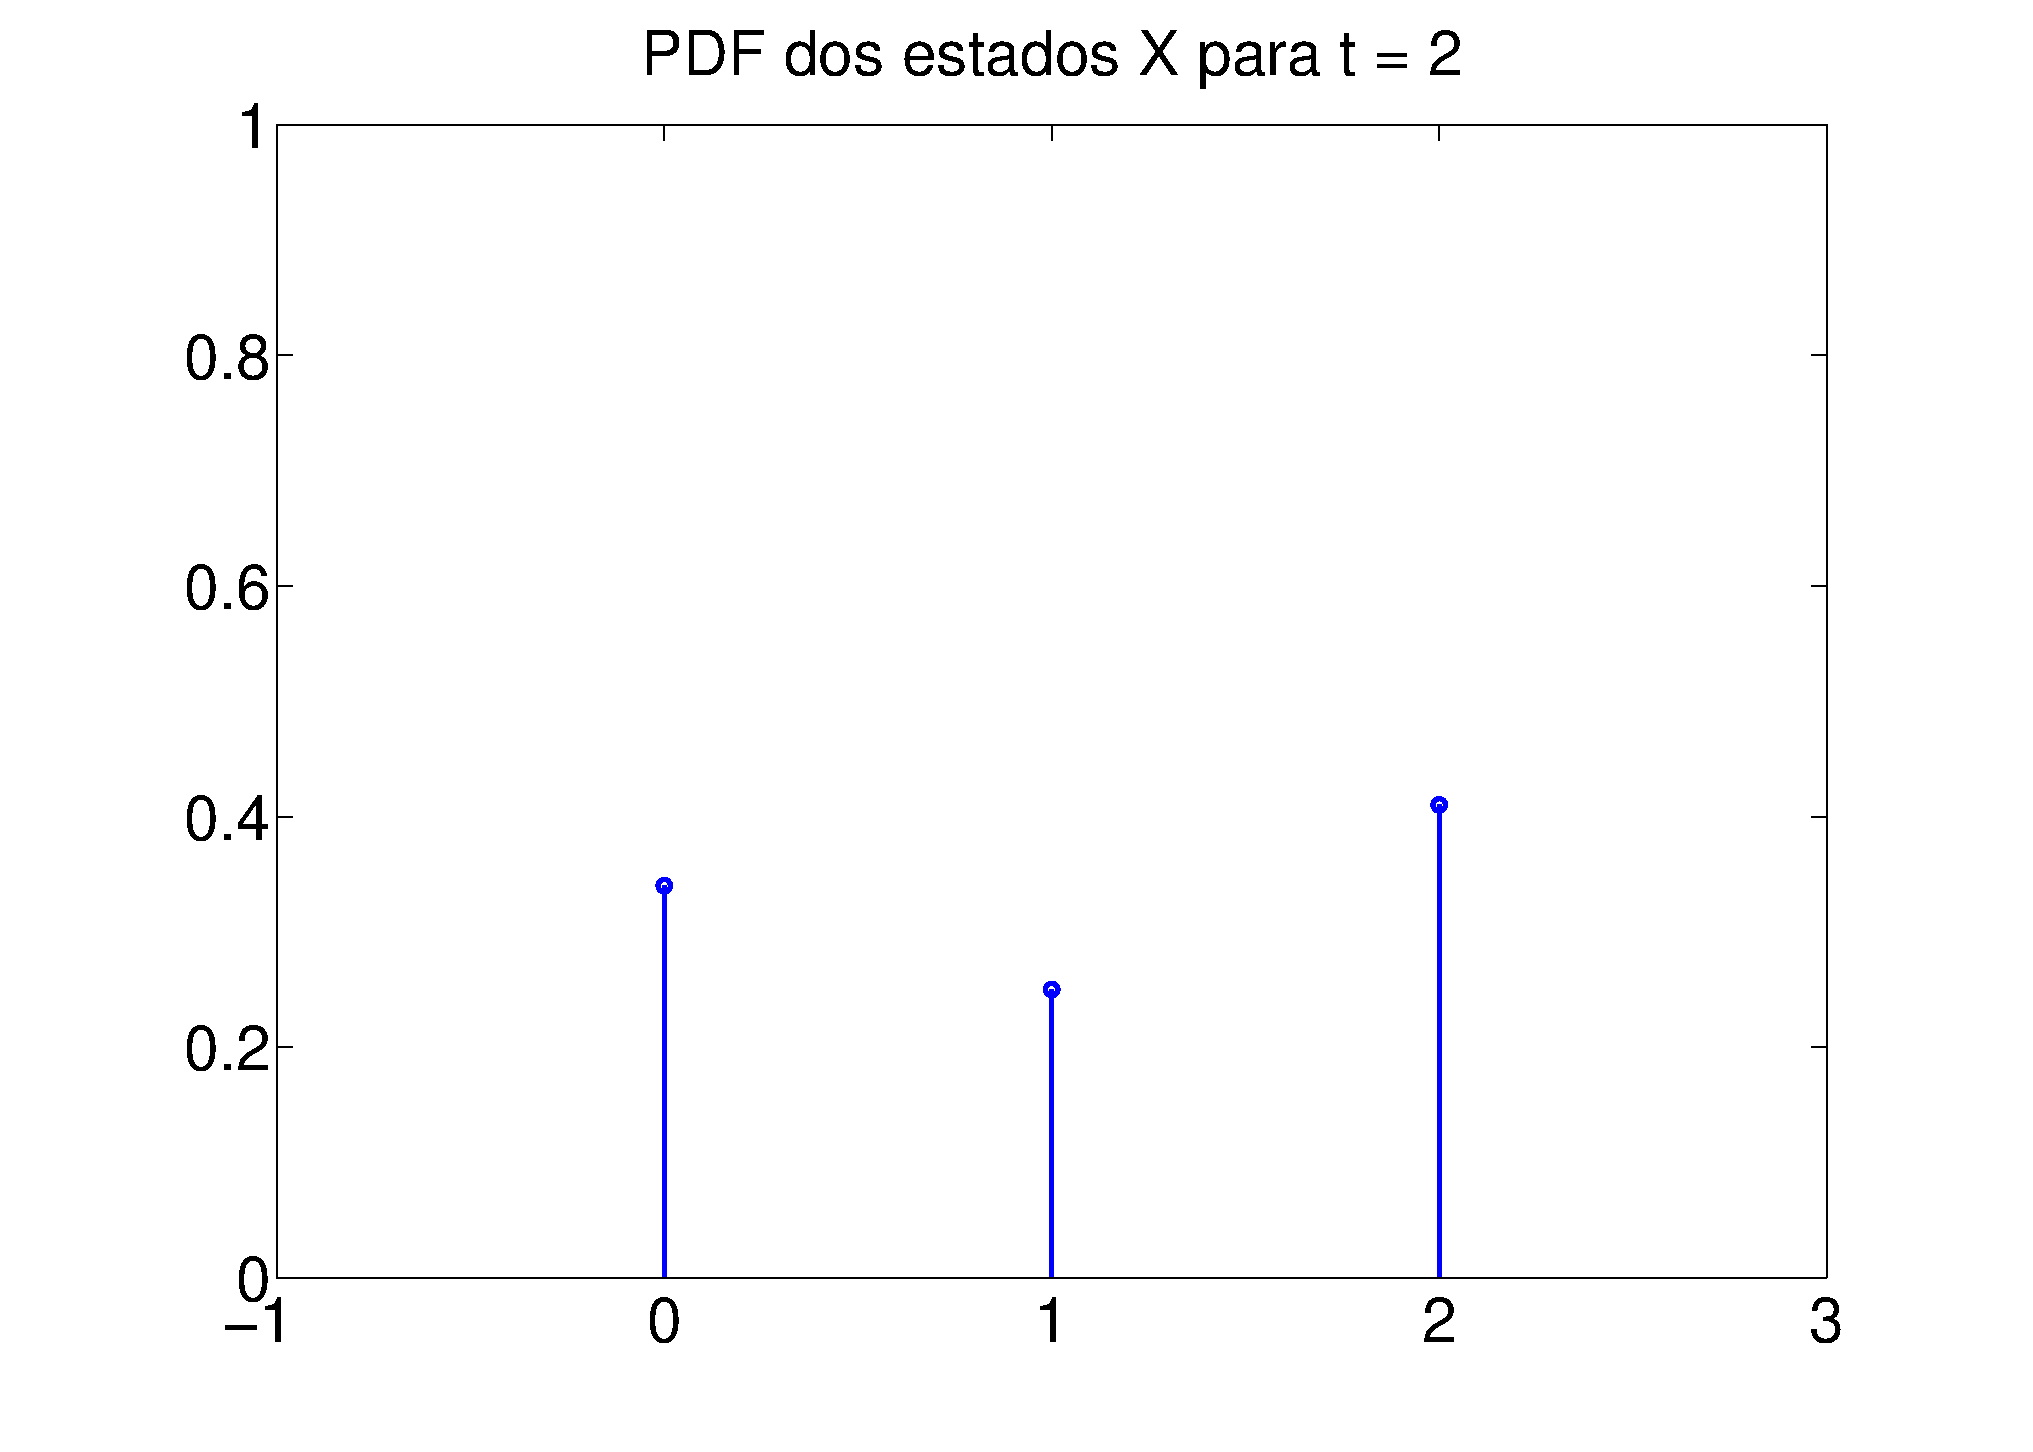
\includegraphics[width = \textwidth]{Q1_d_pdf_x_2}
		\caption{$t = 2$}
	\end{subfigure}
	\begin{subfigure}{0.4\textwidth}
		\centering
		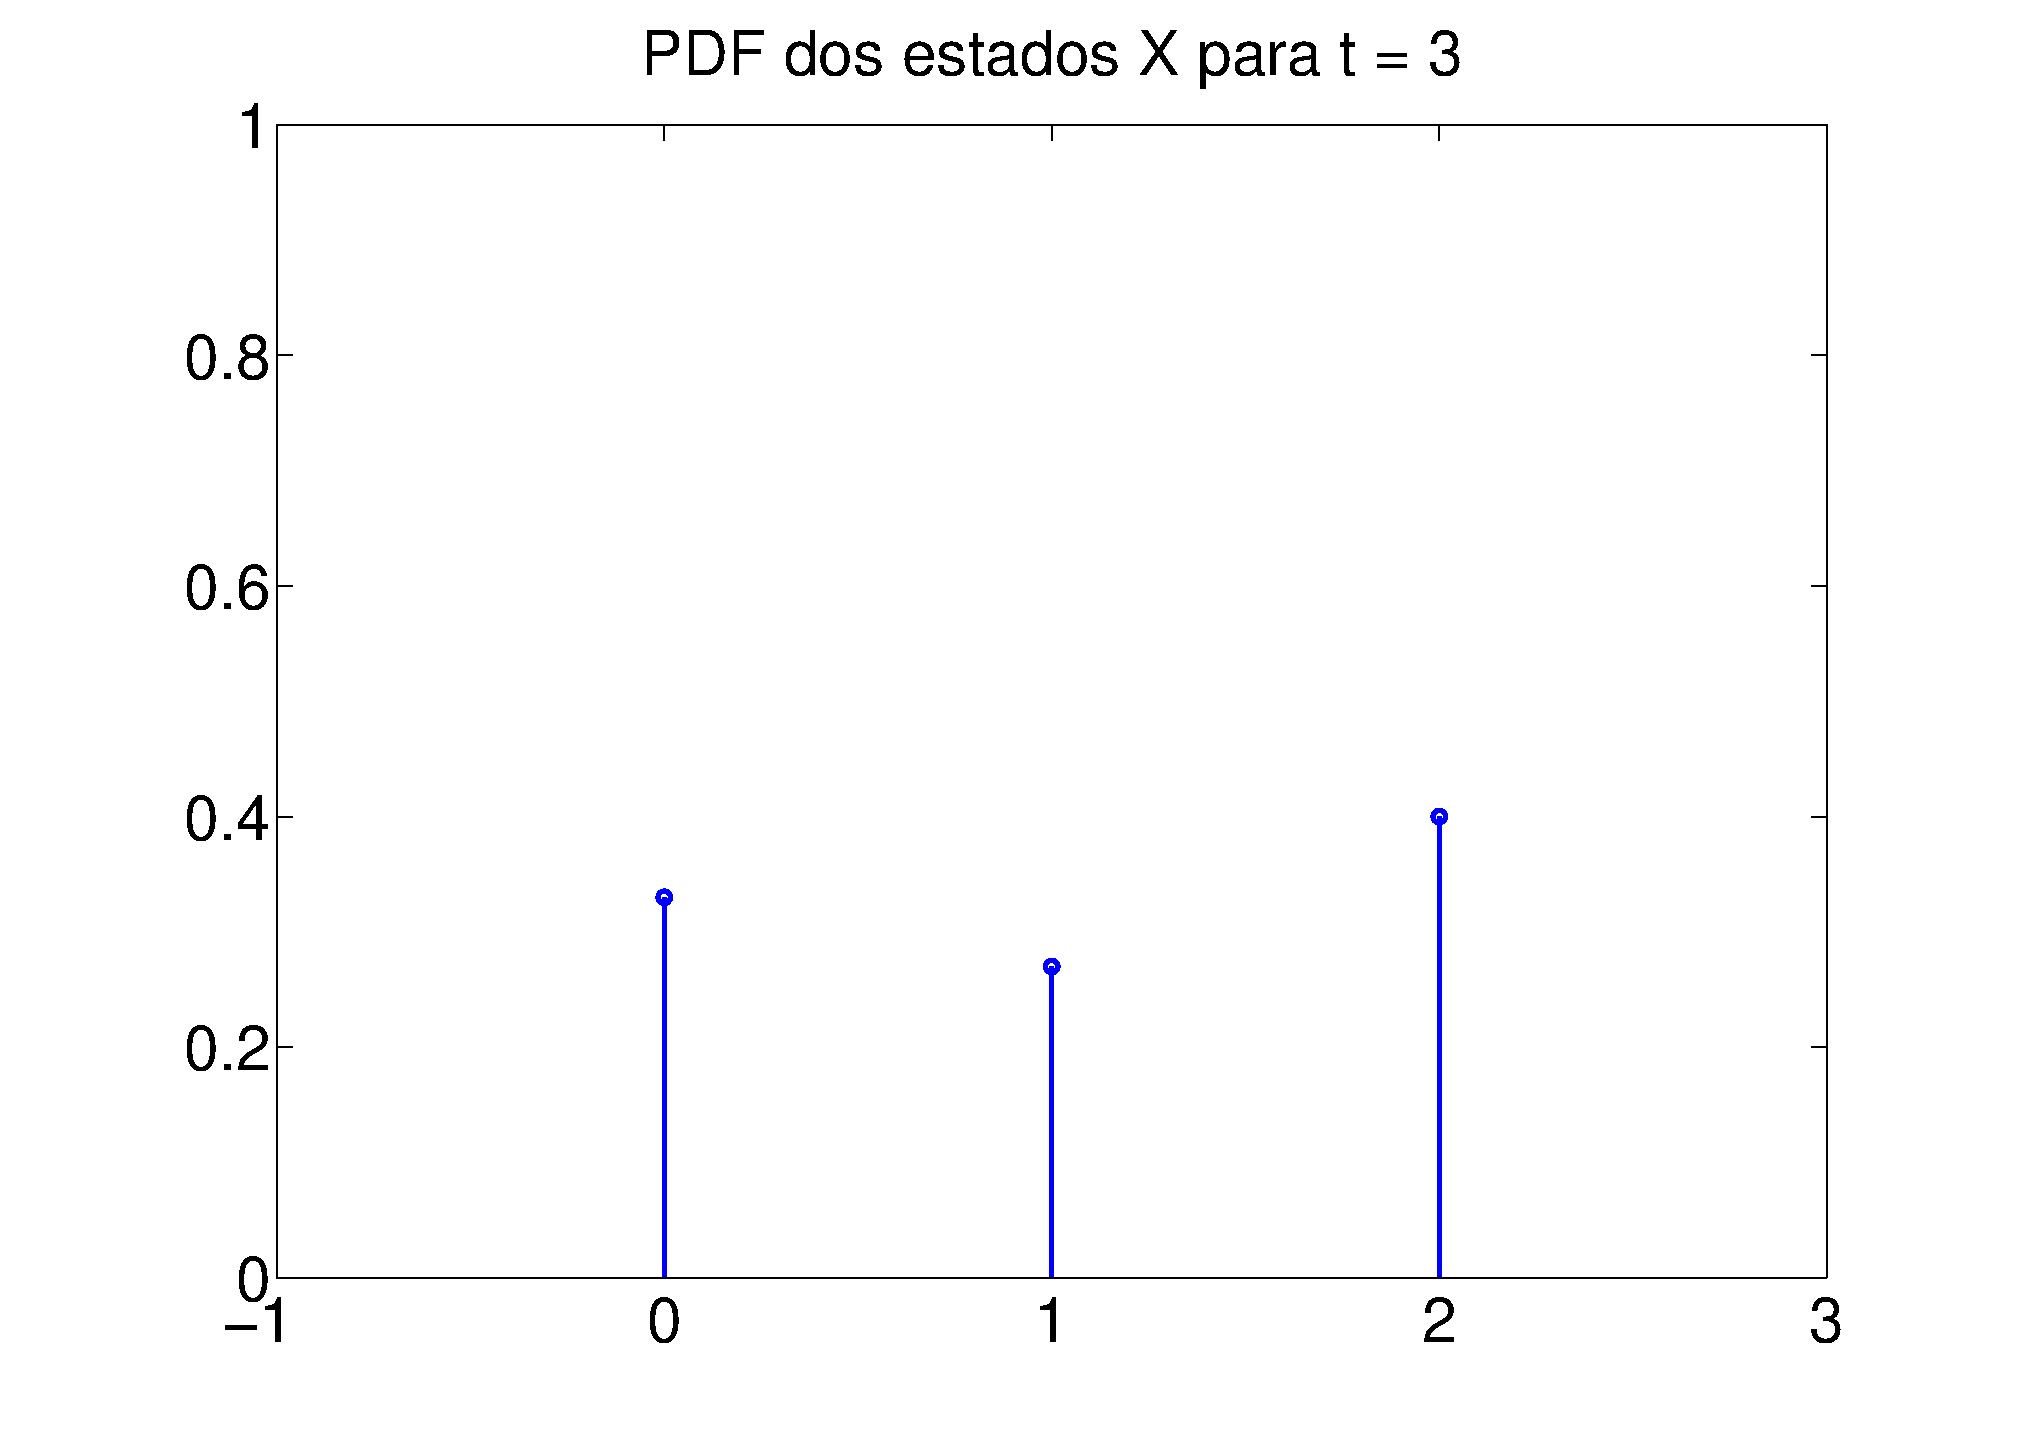
\includegraphics[width = \textwidth]{Q1_d_pdf_x_3}
		\caption{$t = 3$}
	\end{subfigure}
	\caption{Distribuições de $X(t)$}
	\label{pdfs_estados}
\end{figure}

\paragraph{} Como a distribuição inicial dos estados é equiprovável, segue que o histograma do estado $X(0)$ assemelha-se, de fato, a uma distribuição uniforme entre 3 estados. O que se nota, no entanto, nas distribuições dos estados nos instantes seguintes é que eles também se assemelham à distribuição inicial equiprovável. Isso, no entanto, já era esperado, porque o vetor de distribuições inicial $\mathbf{p}_0 = [0.33 \quad 0.33 \quad 0.33]^T$ é, na verdade, o vetor invariante $\boldsymbol{\pi}$ desse processo de Markov (ou seja, ele é o autovetor da matriz de transição $\mathbf{M}$ associado ao autovalor 1; com isso, a transformação $\mathbf{M}$ aplicada a esse autovetor resulta no mesmo vetor). De fato, é possível verificar que o vetor $\boldsymbol{\pi} = [0.33 \quad 0.33 \quad 0.33]^T$ é o vetor invariante, substituindo-o na equação $p_t = \mathbf{M} \times p_{t-1}$:\\

\begin{equation*}
p_t = \left[ \begin{array}{ccc}
0.50 & 0.25 & 0.25 \\ 
0.25 & 0.50 & 0.25 \\ 
0.25 & 0.25 & 0.50 
\end{array} \right] \times \left[\begin{array}{c}
0.33 \\ 
0.33 \\ 
0.33
\end{array} \right] = \left[ \begin{array}{c}
0.33 \\ 
0.33 \\ 
0.33
\end{array}  \right] = \boldsymbol{\pi}
\end{equation*}

\section*{Questão 2}

\textbf{Considere um sistema em que só há 5 estados possíveis: $x = 1$, $x = 2$, $x = 3$, $x = 4$, $x = 5$. Os custos $J(x)$ de cada um dos estados são indicados na tabela abaixo:}\\

\begin{table}[H]
	\centering
	\begin{tabular}{c|c}
	$x$ & $J(x)$ \\ 
	\hline 
	1 & 0.5 \\ 
	\hline 
	2 & 0.2 \\ 
	\hline 
	3 & 0.3 \\ 
	\hline 
	4 & 0.1 \\ 
	\hline 
	5 & 0.4 \\ 
\end{tabular}
\end{table}

\textbf{a) Considere um processo de Markov gerado pela aplicação do algoritmo de Metropolis aos dados da tabela acima, com temperatura fixa $T = 0.1$. Calcule a matriz de transição $\mathbf{M}$ que define o processo $X(t)$.}\\

\textbf{Obs.: note que o estado $X(t)$ é unidimensional, e portanto a matriz $\mathbf{M}$ é 5 x 5.}\\

\paragraph{} Primeiramente, adota-se a seguinte convenção: as colunas da matriz $\mathbf{M}$ correspondem aos estados de origem do processo e que as linhas correspondem aos estados de destino. Dispondo da tabela de estados e $J(x)$, sorteia-se um estado, que não seja o de origem, e calcula-se, para cada estado de origem, o $\Delta J$. No caso do algoritmo de Metropolis, se $\Delta J < 0$, então a transição é aceita imediatamente. Caso contrário, a aceitação segue a seguinte fórmula:\\

\begin{equation*}
\hat{X}(t+1) = \begin{cases}
		  	X(t+1), \quad &\text{se} \  e^{- \frac{(\Delta J)}{T}} > r \\
   		 	X(t), \quad &\text{caso contrário}
		  \end{cases}, \quad \text{onde } r \in (0,1)
\end{equation*}

\paragraph{} Calculando-se, então, os $\Delta J$ referentes ao estado $x = 1$, temos:\\

\begin{align*}
\Delta J_{12} = J(2) - J(1) = 0.2 - 0.5 = - 0.3\\
\Delta J_{13} = J(2) - J(1) = 0.3 - 0.5 = - 0.2\\
\Delta J_{14} = J(2) - J(1) = 0.1 - 0.5 = - 0.4\\
\Delta J_{15} = J(2) - J(1) = 0.4 - 0.5 = - 0.1\\
\end{align*}

\paragraph{} Por $x = 1$ ser o estado de maior valor da função J, a transição para qualquer outro estado resultará em um $\Delta J < 0$, conforme se observa acima. Portanto, todas as transições serão aceitas. Chamando $\mathbf{c}_1$ de o vetor de probabilidades de transição do estado $X(t) = 1$ para $X(t) = j$, chega-se ao seguinte formato para ele:\\

\begin{equation*}
\mathbf{c}_1 = \left[\begin{array}{ccc}
						(4 - \sum_{j \neq i} P(X(t+1) = j \ | \ X(t) = 1)\\
						P(X(t+1) = 2)\\
					 	P(X(t+1) = 3)\\
					 	P(X(t+1) = 4)\\ 
					 	P(X(t+1) = 5)
					\end{array}\right]
\end{equation*}\\

\paragraph{} Aqui, temos que $P(X(t+1) = j) = P(X(t+1) = j \ | \ X(t) = 1) \times P(sortear \ X(t+1) = 2)$. A probabilidade $P(X(t+1) = j \ | \ X(t) = 1)$ é a probabilidade de transição do estado $X(t) = 1$ para $X(t+1) = j$, o qual, por sua vez, é a probabilidade de se aceitar uma transição no algoritmo de Metropolis, dada por $e^{- \frac{(\Delta J)}{T}}$, se $\Delta J > 0$, ou 1, se $\Delta J < 0$. Sendo assim:\\

\begin{equation*}
P(X(t+1) = j \ | \ X(t) = 1) = \begin{cases}
									e^{- \frac{(\Delta J)}{T}}, \quad &\text{se } \Delta J > 0\\
									1, \quad &\text{se } \Delta J < 0
							   \end{cases}
\end{equation*}\\

\paragraph{} Já $P(sortear \ X(t+1) = 2) = \frac{1}{4}$, porque assume-se que não se pode sortear o estado de origem. Com isso, restam 4 estados, os quais têm probabilidade igual de serem sorteados. A probabilidade de permanecer no estado $X(t+1) = 1$ é o complemento da soma das probabilidades de transição, descritas nas outras posições do vetor. Os demais vetores $\mathbf{c}_i, i = 2, 3, 4, 5$, são análogos ao vetor $\mathbf{c}_1$, mudando, somente, no vetor, a posição das probabilidades. Monta-se, então, a matriz de transição $\mathbf{M} = [\mathbf{c}_1 \quad \mathbf{c}_2 \quad \mathbf{c}_3 \quad \mathbf{c}_4 \quad \mathbf{c}_5]$. Após calcular cada uma dessas probabilidades, chega-se na matriz $\mathbf{M}$ final, exibida abaixo:\\

\begin{equation*}
\mathbf{M} = \left[ 
\begin{array}{ccccc}
0 & 0.0124 & 0.0338 & 0.0046 & 0.0920 \\ 
0.2500 & 0.6117 & 0.2500 & 0.0920 & 0.2500 \\ 
0.2500 & 0.0920 & 0.3742 & 0.0338 & 0.2500 \\ 
0.2500 & 0.2500 & 0.2500 & 0.8572 & 0.2500 \\ 
0.2500 & 0.0338 & 0.0920 & 0.0124 & 0.1580
\end{array} \right]
\end{equation*}\\

%%%%%%%%%%%%%%%%%%%%%%%%%%%%%%%%%%%%% O TRECHO ABAIXO ESTÁ COMENTADO %%%%%%%%%%%%%%%%%%%%%%%%%%%%%%%%%%

\begin{comment}
\begin{equation}
\mathbf{M} = \left[
\begin{smallmatrix}
(4 - \sum_{j \neq i} P(X(t+1) = j \ | \ X(t) = 1) & P(X(t+1) = 1 \ | \ X(t) = 2) \times P(sortear \ X(t+1) = 1) & P(X(t+1) = 1 \ | \ X(t) = 3) \times P(sortear \ X(t+1) = 1) & P(X(t+1) = 1 \ | \ X(t) = 1) \times P(sortear \ X(t+1) = 1) & P(X(t+1) = 1 \ | \ X(t) = 5) \times P(sortear \ X(t+1) = 5) \\ 
P(X(t+1) = 2 \ | \ X(t) = 1) \times P(sortear \ X(t+1) = 2) & (4 - \sum_{j \neq i} P(X(t+1) = j \ | \ X(t) = 2) & P(X(t+1) = 2 \ | \ X(t) = 3) \times P(sortear \ X(t+1) = 3) & P(X(t+1) = 2 \ | \ X(t) = 4) \times P(sortear \ X(t+1) = 4) & P(X(t+1) = 2 \ | \ X(t) = 5) \times P(sortear \ X(t+1) = 5) \\ 
P(X(t+1) = 3 \ | \ X(t) = 1) \times P(sortear \ X(t+1) = 3) & P(X(t+1) = 3 \ | \ X(t) = 2) \times P(sortear \ X(t+1) = 3) & (4 - \sum_{j \neq i} P(X(t+1) = j \ | \ X(t) = 3) & P(X(t+1) = 3 \ | \ X(t) = 4) \times P(sortear \ X(t+1) = 3) & P(X(t+1) = 3 \ | \ X(t) = 5) \times P(sortear \ X(t+1) = 3) \\ 
P(X(t+1) = 4 \ | \ X(t) = 1) \times P(sortear \ X(t+1) = 4) & P(X(t+1) = 4 \ | \ X(t) = 2) \times P(sortear \ X(t+1) = 4) & P(X(t+1) = 4 \ | \ X(t) = 3) \times P(sortear \ X(t+1) = 4) & (4 - \sum_{j \neq i} P(X(t+1) = j \ | \ X(t) = 4) & P(X(t+1) = 4 \ | \ X(t) = 5) \times P(sortear \ X(t+1) = 4) \\ 
P(X(t+1) = 5 \ | \ X(t) = 1) \times P(sortear \ X(t+1) = 5) & P(X(t+1) = 5 \ | \ X(t) = 2) \times P(sortear \ X(t+1) = 5) & P(X(t+1) = 5 \ | \ X(t) = 3) \times P(sortear \ X(t+1) = 5) & P(X(t+1) = 5 \ | \ X(t) = 4) \times P(sortear \ X(t+1) = 5) & (4 - \sum_{j \neq i} P(X(t+1) = j \ | \ X(t) = 5)
\end{smallmatrix} \right]
\end{equation}
\end{comment}

%%%%%%%%%%%%%%%%%%%%%%%%%%%%%% FIM DO TRECHO COMENTADO %%%%%%%%%%%%%%%%%%%%%%%%%%%%%%%%%%%%%%%%%%%%%

\textbf{b) Iniciando em $X(0) = 1$, calcule manualmente 4 amostras do processo $X(t)$.}\\

\paragraph{} Como $X(0) = 1$, segue que $\mathbf{p}_0 = [1 \quad 0 \quad 0 \quad 0 \quad 0]^T$. A distribuição de probabilidades $\mathbf{p}_1$ é, então, calculada, utilizando a matriz de transição $\mathbf{M}$ obtida no item anterior.\\

\begin{equation*}
\mathbf{p}_1 = \mathbf{M} \times \mathbf{p}_0 = \left[ 
\begin{array}{ccccc}
0 & 0.0124 & 0.0338 & 0.0046 & 0.0920 \\ 
0.2500 & 0.6117 & 0.2500 & 0.0920 & 0.2500 \\ 
0.2500 & 0.0920 & 0.3742 & 0.0338 & 0.2500 \\ 
0.2500 & 0.2500 & 0.2500 & 0.8572 & 0.2500 \\ 
0.2500 & 0.0338 & 0.0920 & 0.0124 & 0.1580
\end{array} \right] \times \left[\begin{array}{c}
1 \\ 
0 \\ 
0 \\ 
0 \\ 
0
\end{array} \right] =  \left[\begin{array}{c}
0 \\ 
0.2500 \\ 
0.2500 \\ 
0.2500 \\ 
0.2500
\end{array} \right]
\end{equation*}\\

\paragraph{} Sorteia-se, então, uma amostra da distribuição $\mathbf{p}_1$. Para tal, adota-se a mesma abordagem utilizada no item (b) da questão 1: sorteia-se um número da distribuição uniforme (0,1) e ele é mapeado em algum estado possível, seguindo a CDF obtida do vetor $\mathbf{p}_1$. Para essa iteração, o mapeamento está exibido abaixo. A extensão para as iterações subsequentes é direta, alterando, somente, os intervalos em que cada estado é mapeado, respeitando a CDF em questão, e, portanto, ela será omitida.\\

\begin{equation*}
X(1) = \begin{cases}
			2, \quad r \leq 0.25\\
			3, \quad 0.25 < r \leq 0.5\\
			4, \quad 0.5 < r \leq 0.75\\
			5, \quad r > 0.75
	   \end{cases}, \quad r \in (0,1)
\end{equation*}\\

\paragraph{} Sorteando $r = 0,8$, chega-se no estado $X(1) = 5$. Iniciando a segunda iteração, calcula-se $\mathbf{p}_2$:\\

\begin{equation*}
\mathbf{p}_2 = \left[ 
\begin{array}{ccccc}
0 & 0.0124 & 0.0338 & 0.0046 & 0.0920 \\ 
0.2500 & 0.6117 & 0.2500 & 0.0920 & 0.2500 \\ 
0.2500 & 0.0920 & 0.3742 & 0.0338 & 0.2500 \\ 
0.2500 & 0.2500 & 0.2500 & 0.8572 & 0.2500 \\ 
0.2500 & 0.0338 & 0.0920 & 0.0124 & 0.1580
\end{array} \right] \times \left[\begin{array}{c}
0 \\ 
0.2500 \\ 
0.2500 \\ 
0.2500 \\ 
0.2500
\end{array} \right] =  \left[\begin{array}{c}
0.0357 \\ 
0.3009 \\ 
0.1875 \\ 
0.4018 \\
0.0741
\end{array} \right]
\end{equation*}\\

\paragraph{} Sorteando $r = 0,6$, obtém-se $X(2) = 4$. Começa-se, então, a terceira iteração:\\

\begin{equation*}
\mathbf{p}_3 = \left[ 
\begin{array}{ccccc}
0 & 0.0124 & 0.0338 & 0.0046 & 0.0920 \\ 
0.2500 & 0.6117 & 0.2500 & 0.0920 & 0.2500 \\ 
0.2500 & 0.0920 & 0.3742 & 0.0338 & 0.2500 \\ 
0.2500 & 0.2500 & 0.2500 & 0.8572 & 0.2500 \\ 
0.2500 & 0.0338 & 0.0920 & 0.0124 & 0.1580
\end{array} \right] \times \left[\begin{array}{c}
0.0357 \\ 
0.3009 \\ 
0.1875 \\ 
0.4018 \\
0.0741
\end{array} \right] =  \left[\begin{array}{c}
0.0187 \\ 
0.2954 \\ 
0.1389 \\ 
0.4940 \\
0.0531
\end{array} \right]
\end{equation*}\\

\paragraph{} Sorteando $r = 0,8$, resulta em $X(3) = 4$. As 4 primeiras amostras do processo são, portanto, $\mathbf{x} = [X(0) \quad X(1) \quad X(2) \quad X(3)] = [1 \quad 5 \quad 4 \quad 4]$.

\textbf{c) Qual é o vetor invariante da matriz $\mathbf{M}$ do item (a)?}\\

\textbf{Obs.: para facilitar os cálculos, pode-se usar o computador neste item.}\\

\paragraph{} O vetor invariante $\boldsymbol{\pi}$ é aquele associado ao autovalor 1 da matriz de transição $\mathbf{M}$. Isso significa que quando a matriz $\mathbf{M}$ é aplicada nesse vetor, o vetor resultante é ele próprio, ou seja, a distribuição dos estados, para instantes $t$ subsequentes não se altera mais. O código que calcula o vetor invariante é exibido a seguir:\\

\begin{lstlisting}
%% Montagem da matriz de transição M

C1 = [0 1/4 1/4 1/4 1/4]';
C2 = [exp(-3)/4 (3-exp(-3)-exp(-2)-exp(-1))/4 exp(-1)/4 1/4 exp(-2)/4]';
C3 = [exp(-2)/4 1/4 (2-exp(-2)-exp(-1))/4 1/4 exp(-1)/4]';
C4 = [exp(-4)/4 exp(-1)/4 exp(-2)/4 (4-exp(-4)-exp(-3)-exp(-2)-exp(-1))/4 exp(-3)/4]';
C5 = [exp(-1)/4 1/4 1/4 1/4 (1-exp(-1))/4]';

M = [C1 C2 C3 C4 C5];

%% Inicialização p0

p0 = zeros(1,5)';

% Geração aleatória de p0

r = rand();
b = 1;

for i = 1:(length(p0)-1)
    p0(i) = r;
    c = b - r;
    p0(i+1) = c;
    r = random('unif', 0, c);
    b = c;
end

%% Cálculo do vetor invariante

p_atual = p0;
contador = 1;

while(true)
    p_seguinte = M * p_atual;
    if norm((p_seguinte - p_atual), 2) == 0
        break
    end
    p_atual = p_seguinte;
    contador = contador + 1;
end

p_inv = p_atual
contador

% Resultados
% 
% p_inv =
% 
%     0.0117
%     0.2341
%     0.0861
%     0.6364
%     0.0317
% 
% 
% contador =
% 
%     84
\end{lstlisting}

\paragraph{} O vetor invariante, para o qual o processo de Markov em questão converge, é, portanto, $\boldsymbol{\pi} = [0.0117 \quad 0.2341 \quad 0.0861 \quad 0.6364 \quad 0.0317]^T$. A velocidade com a qual a convergência é alcançada depende do estado inicial $\mathbf{p}_0$. Rodando esse código algumas vezes, notou-se que, em média, são necessárias 83 iterações ($t = 83$) para se alcançar o vetor invariante.\\

\textbf{d) Calcule os fatores de Boltzmann (ou seja, $e^{-(J(x))/T}$) associados aos dados da tabela acima, e compare-os com o resultado do item (c). Use $T = 0.1$.}\\

\paragraph{} A Tabela \ref{tabela_fatores_boltzmann} exibe os fatores de Boltzmann calculados para cada valor da função custo $J(x)$:\\

\begin{table}[H]
	\centering
	\begin{tabular}{c|c|c}
	$x$ & $J(x)$ & $e^{- \frac{J(x)}{T}}$ \\ 
	\hline 
	1 & 0.5 & 0.0067 \\ 
	\hline 
	2 & 0.2 & 0.1353 \\ 
	\hline 
	3 & 0.3 & 0.0498 \\ 
	\hline 
	4 & 0.1 & 0.3679 \\ 
	\hline 
	5 & 0.4 & 0.0183 \\ 
	\end{tabular} 
	\caption{Tabela com os fatores de Boltzmann calculados para cada $J(x)$}
	\label{tabela_fatores_boltzmann}
\end{table}

\paragraph{} Nota-se que os maiores fatores de Boltzmann estão associados aos menores valores da função $J(x)$, enquanto que os menores fatores encontram-se associados aos maiores valores dessa função. Isso é esperado, já que os estados mais prováveis são aqueles que resultam nos menores valores de $J(x)$. Isso é confirmado através da transformação desses fatores de Boltzmann em uma distribuição, conforme exibido na Tabela \ref{tabela_distribuicao_boltzmann}.\\

\begin{table}
	\centering
	\begin{tabular}{c|c|c}
	$e^{- \frac{J(x)}{T}}$ & $p = \frac{e^{- \frac{J(x)}{T}}}{\sum_{i = 1}^{5} e^{- \frac{J(x_i)}{T}}}$ & $\boldsymbol{\pi}$ \\ 
	\hline 
	0.0067 & 0.0117 & 0.0117\\ 
	\hline 
	0.1353 & 0.2341 & 0.2341\\ 
	\hline 
	0.0498 & 0.0861 & 0.0861\\ 
	\hline 
	0.3679 & 0.6364 & 0.6364\\ 
	\hline 
	0.0183 & 0.0317 & 0.0317\\ 
	\end{tabular} 
	\caption{Tabela com os fatores de Boltzmann transformados em uma distribuição}
	\label{tabela_distribuicao_boltzmann}
\end{table}

\paragraph{} O que se observa, também, é que o vetor correspondente aos fatores de Boltzmann transformados em uma distribuição é igual ao vetor invariante $\boldsymbol{\pi}$, calculado no item (c). De fato, o vetor invariante é a distribuição de estados para a qual o processo de Markov converge. Lembrando que ao executar o algoritmo de Metropolis um número suficiente de vezes, a distribuição de estados também converge para uma distribuição, que é, justamente, a distribuição de Boltzmann. Sendo assim, o vetor invariante $\boldsymbol{\pi}$ corresponde, na verdade, à distribuição de Boltzmann, o que explica a igualdade entre ambos.\\

\textbf{e) \textit{Simulated Annealing}: Usando um computador, execute 1000 iterações do algoritmo de Metropolis em cada uma das 10 temperaturas a seguir. Na passagem de uma temperatura para a outra, use o estado atual. Comente as distribuições de probabilidade obtidas no final de cada temperatura.}\\

\begin{table}[H]
	\centering
	\begin{tabular}{c|c|c|c|c|c|c|c|c|c}
	$T_0$ & $T_1$ & $T_2$ & $T_3$ & $T_4$ & $T_5$ & $T_6$ & $T_7$ & $T_8$ & $T_9$ \\ 
	\hline 
	0.1000 & 0.0631 & 0.0500 & 0.0431 & 0.0387 & 0.0356 & 0.0333 & 0.0315 & 0.0301 & 0.0289 \\ 
\end{tabular} 
\end{table}

\paragraph{} O código, em MATLAB, que implementa o Simulated Annealing para esse problema é exibido a seguir.\\

\begin{lstlisting}
T = [0.100 0.0631 0.0500 0.0431 0.0387 0.0356 0.0333 0.0315 0.0301 0.0289];
J = [0.5 0.2 0.3 0.1 0.4];
x_atual = random('unid',5); % Estado inicial aleatório
J_atual = J(x_atual);
J_min = Inf;
N = 1000;
X = zeros(length(T), N);
custos = zeros(length(T), N);

for k = 1:length(T)
    for n = 1:N
        x_futuro = random('unid',5);
        J_futuro = J(x_futuro);
        delta_J = J_futuro - J_atual;

        if delta_J < 0
            x_atual = x_futuro;
            J_atual = J_futuro;
        else
            r = rand();
            if r < exp(-(delta_J)/T(k))
                x_atual = x_futuro;
                J_atual = J_futuro;
            end
        end

        if J_atual < J_min
            J_min = J_atual;
            x_min = x_atual;
        end
        
        X(k, n) = x_atual;
        custos(k, n) = J_atual;
    end
end

for k = 1:length(T)
    figure(k)
    hist(X(k, (N-100):end), [0 1 2 3 4 5 6])
    axis([0 6 0 100])
    set(gca, 'FontSize', 30)
    title(['Histograma dos 100 últimos estados X para T = ' num2str(T(k))], 'FontSize', 30)
end
\end{lstlisting}

\paragraph{} Os histogramas dos estados obtidos ao final de cada temperatura encontram-se na Figura \ref{histogramas_estados_temperaturas}. Como era de se esperar, os estados mais prováveis são os dois de menor energia ($x = 2$ e $x = 4$) e, ao longo das temperaturas, eles vão ficando cada vez mais prováveis, indicando que o processo está convergindo para o ponto de mínimo. Tal convergência se verifica, especialmente, nas últimas temperaturas, nas quais sorteou-se, somente, os estados de menor energia.\\

\begin{figure}
	\centering
	\begin{subfigure}{0.32\textwidth}
		\centering
		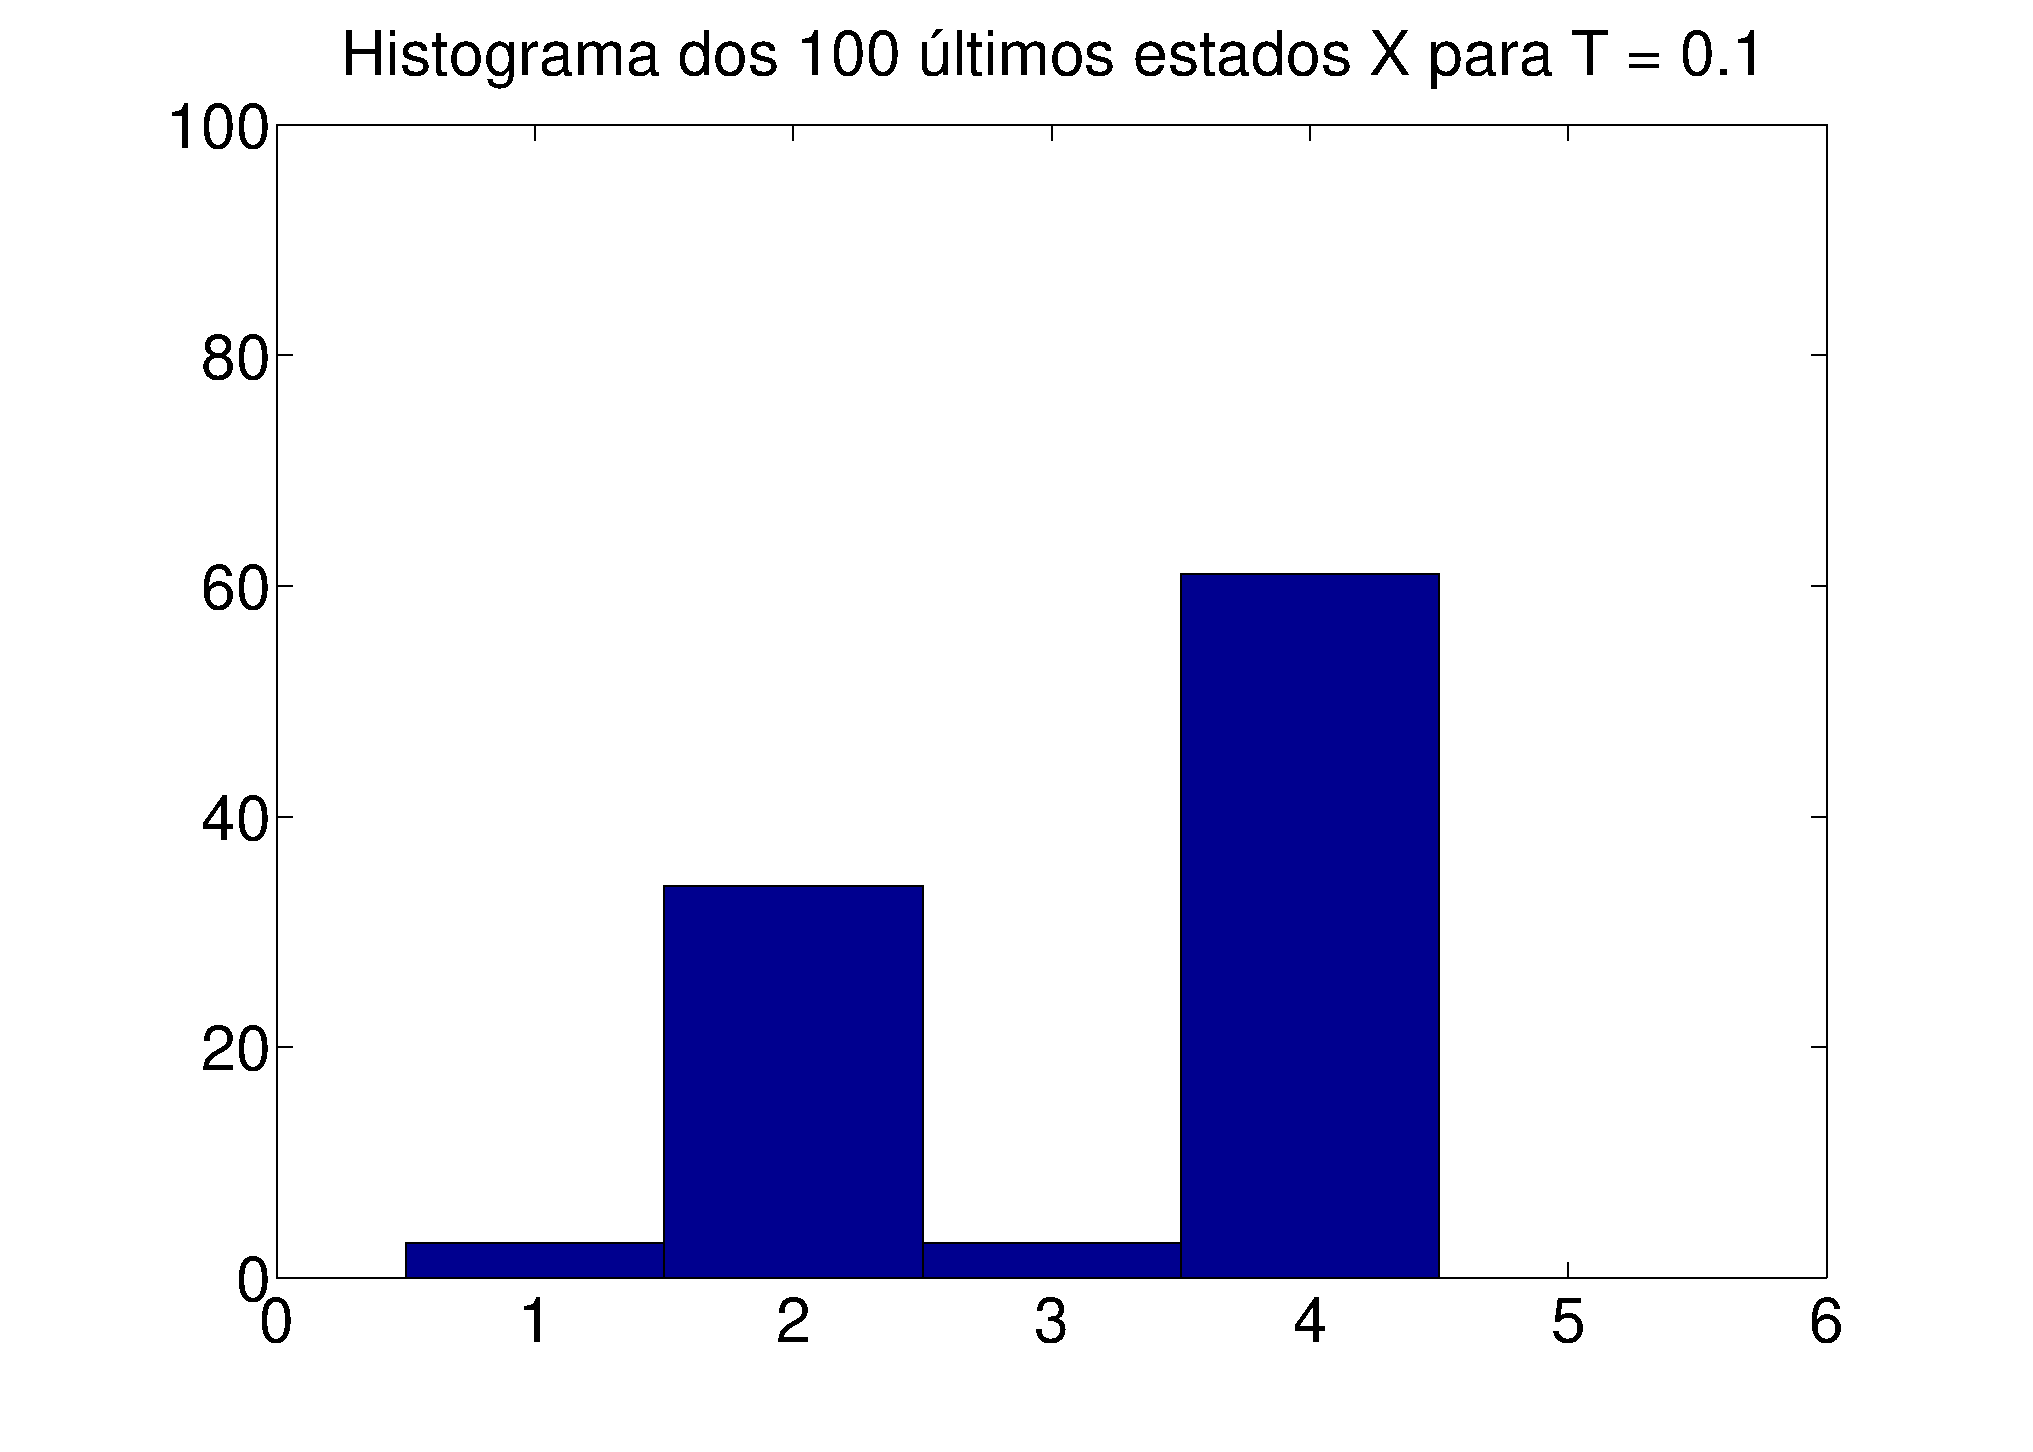
\includegraphics[width = \textwidth]{Q2_e_histograma_x_t_1}
		\caption{$T = 0.1$}
	\end{subfigure}
		\begin{subfigure}{0.32\textwidth}
		\centering
		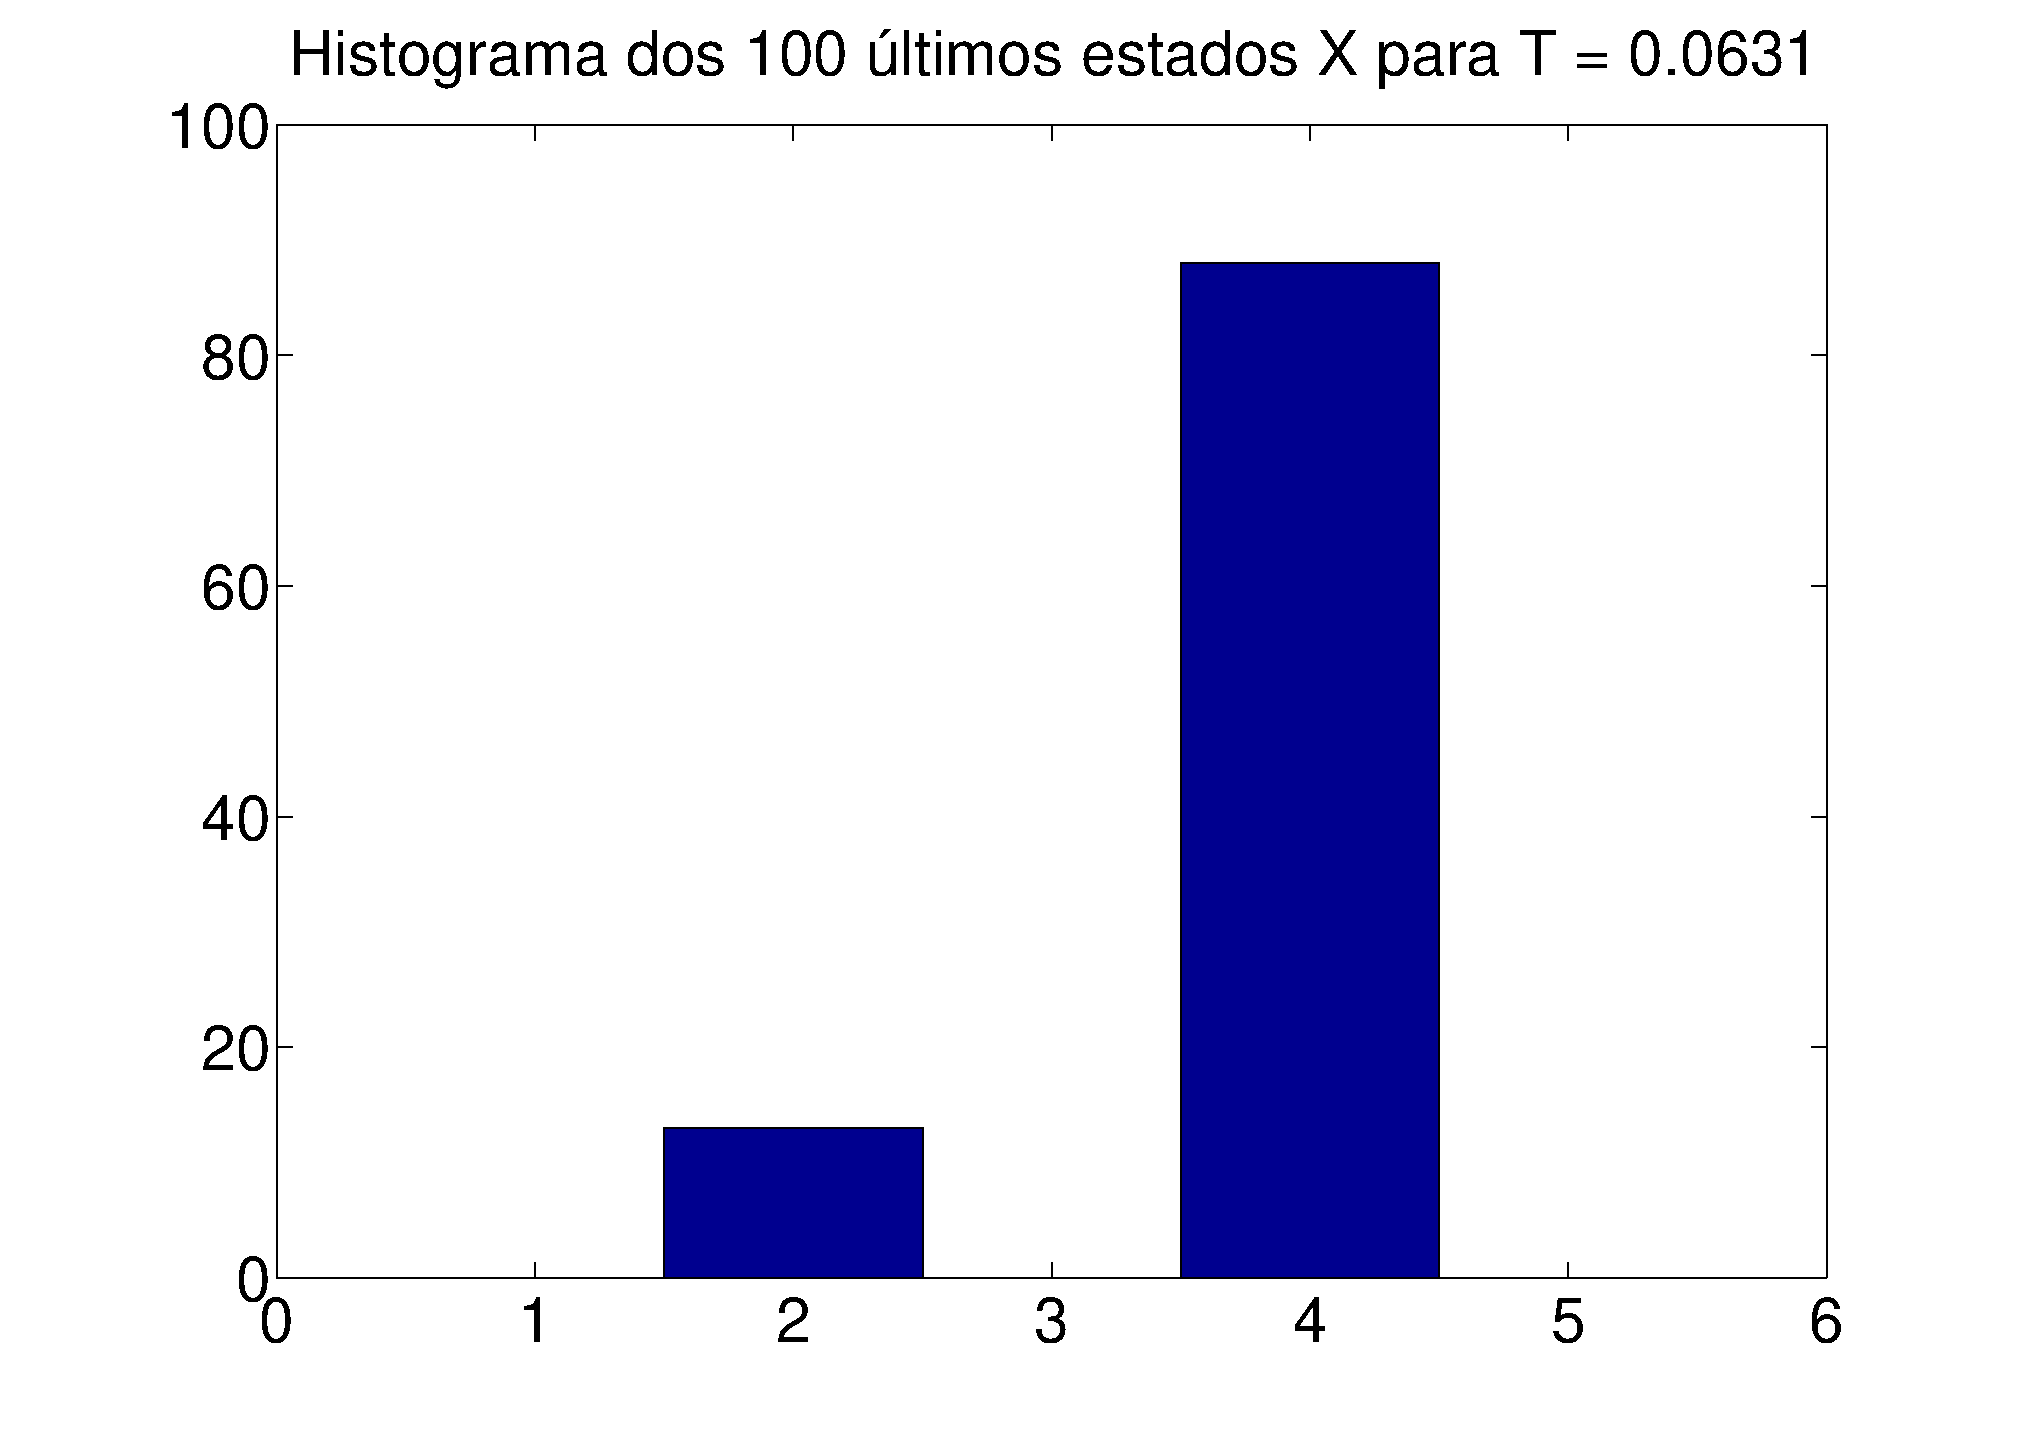
\includegraphics[width = \textwidth]{Q2_e_histograma_x_t_2}
		\caption{$T = 0.0631$}
	\end{subfigure}
		\begin{subfigure}{0.32\textwidth}
		\centering
		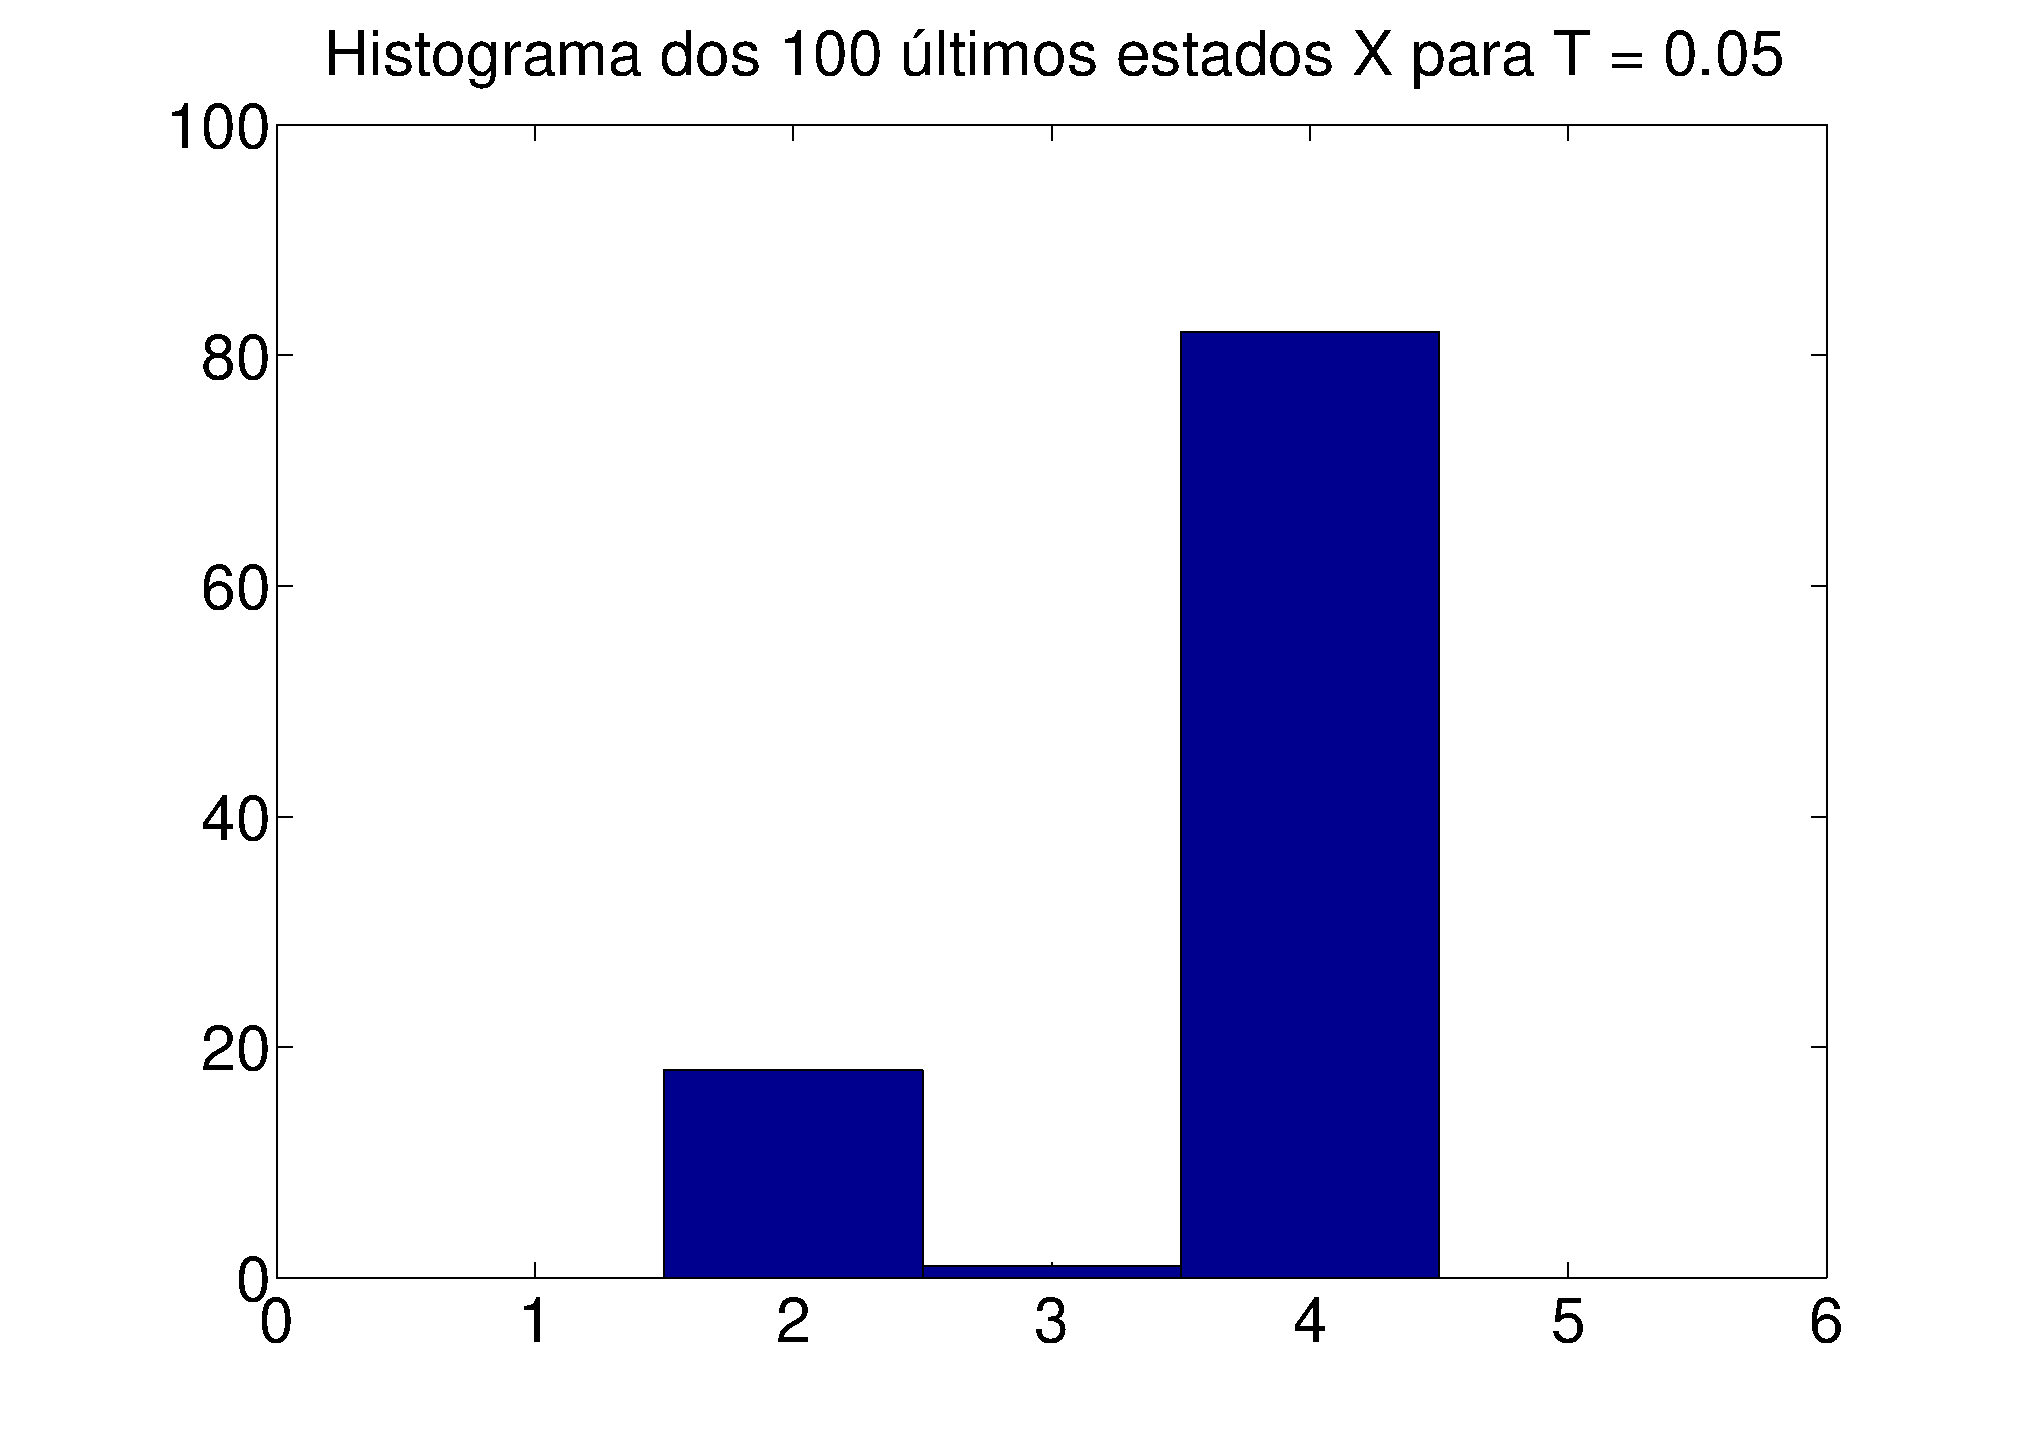
\includegraphics[width = \textwidth]{Q2_e_histograma_x_t_3}
		\caption{$T = 0.05$}
	\end{subfigure}
		\begin{subfigure}{0.32\textwidth}
		\centering
		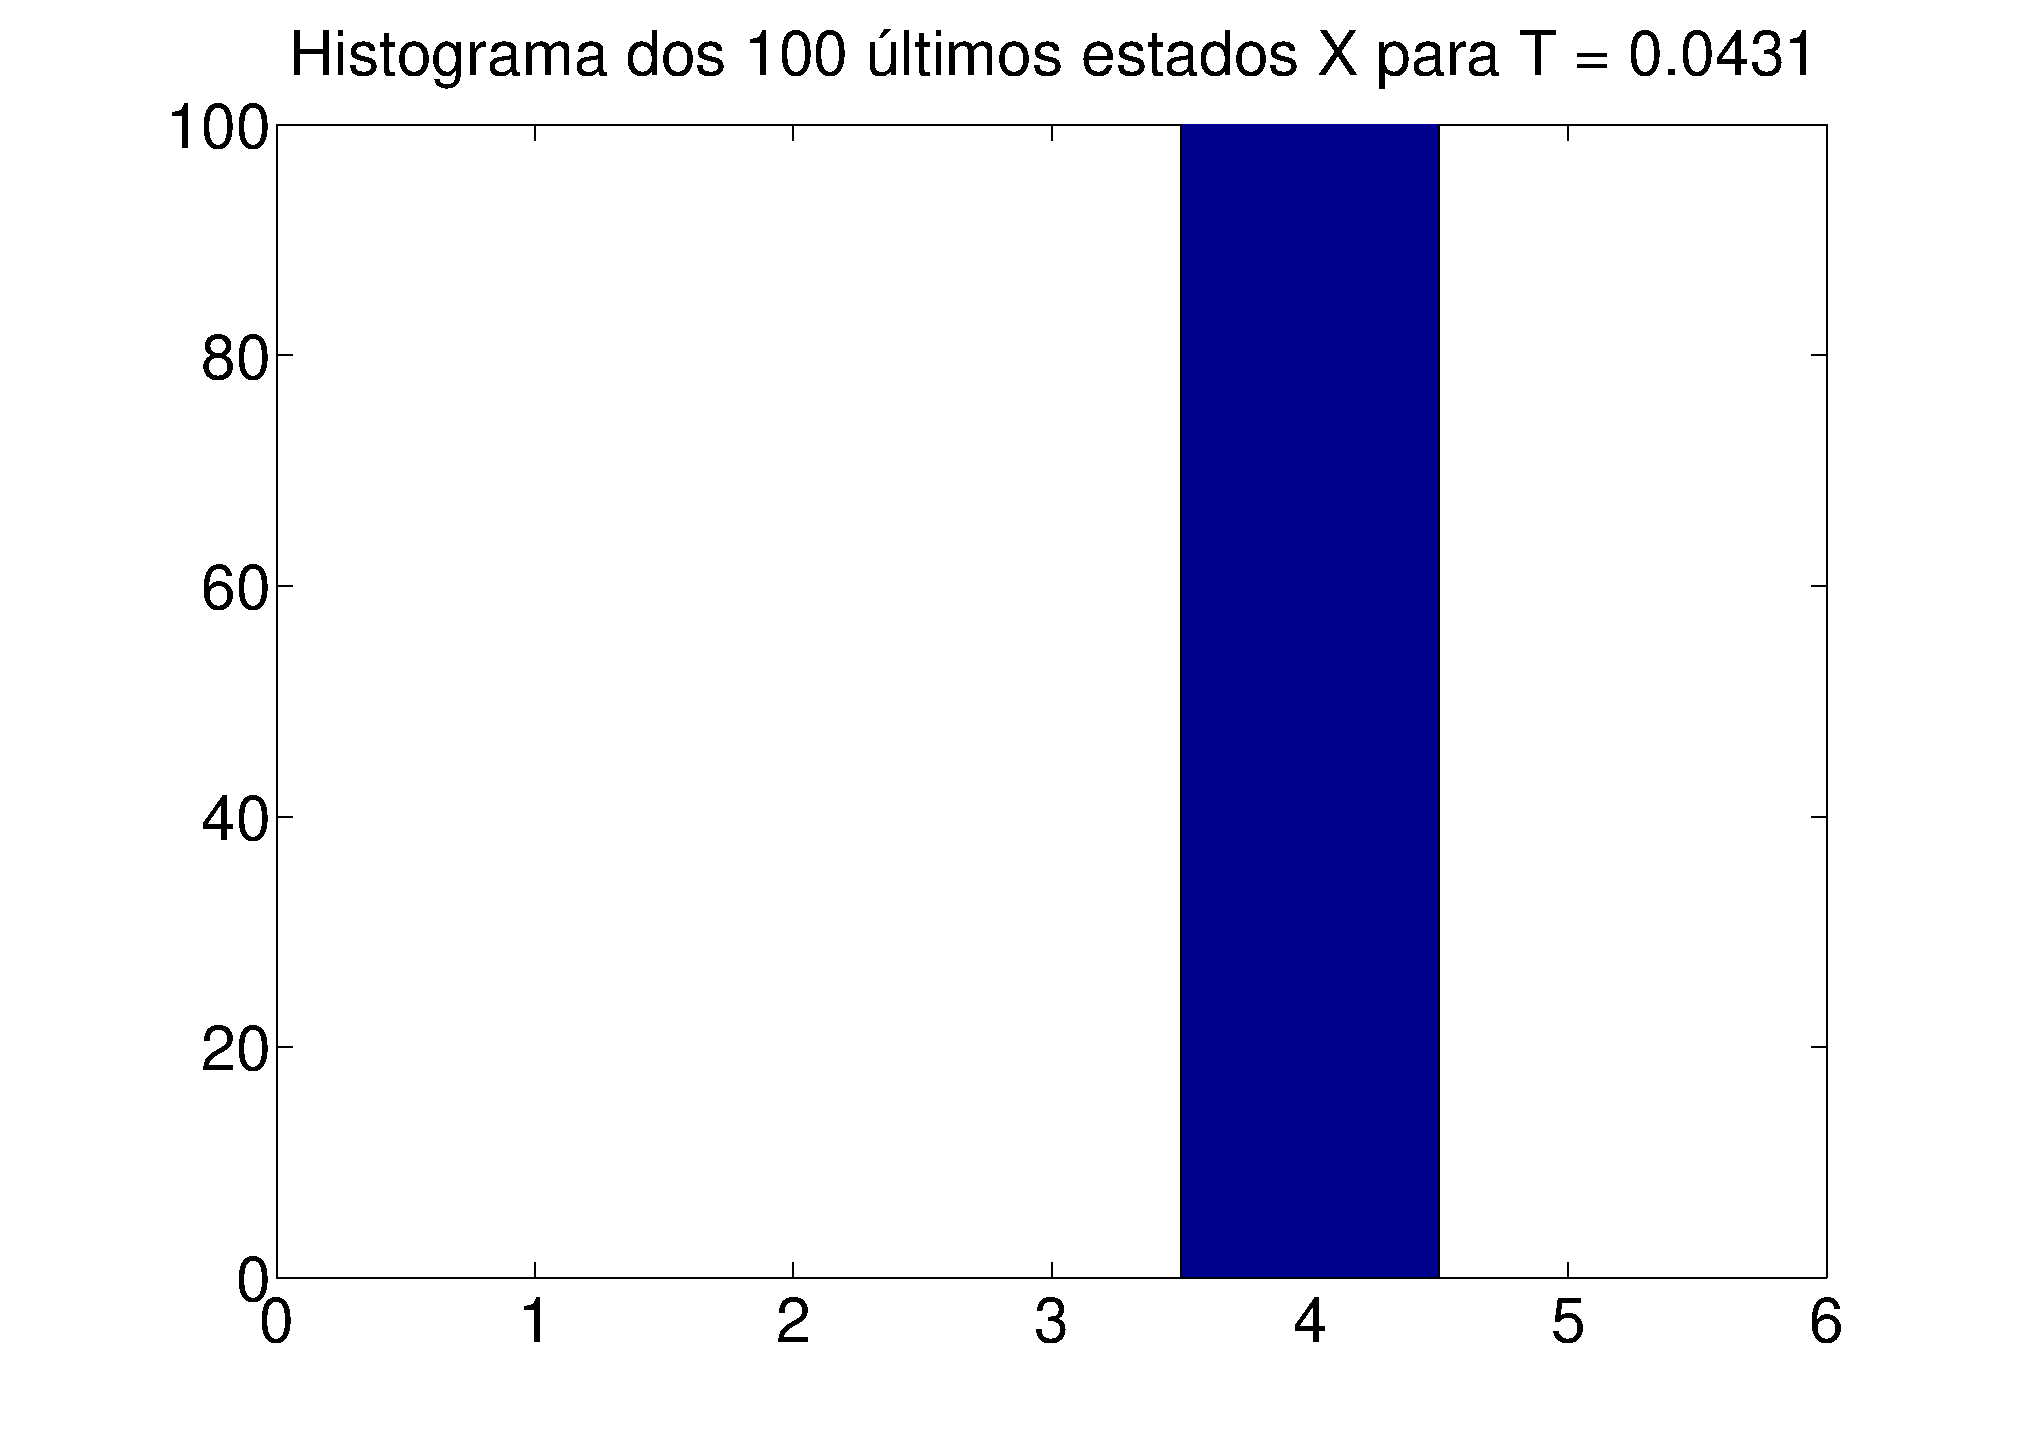
\includegraphics[width = \textwidth]{Q2_e_histograma_x_t_4}
		\caption{$T = 0.0431$}
	\end{subfigure}
		\begin{subfigure}{0.32\textwidth}
		\centering
		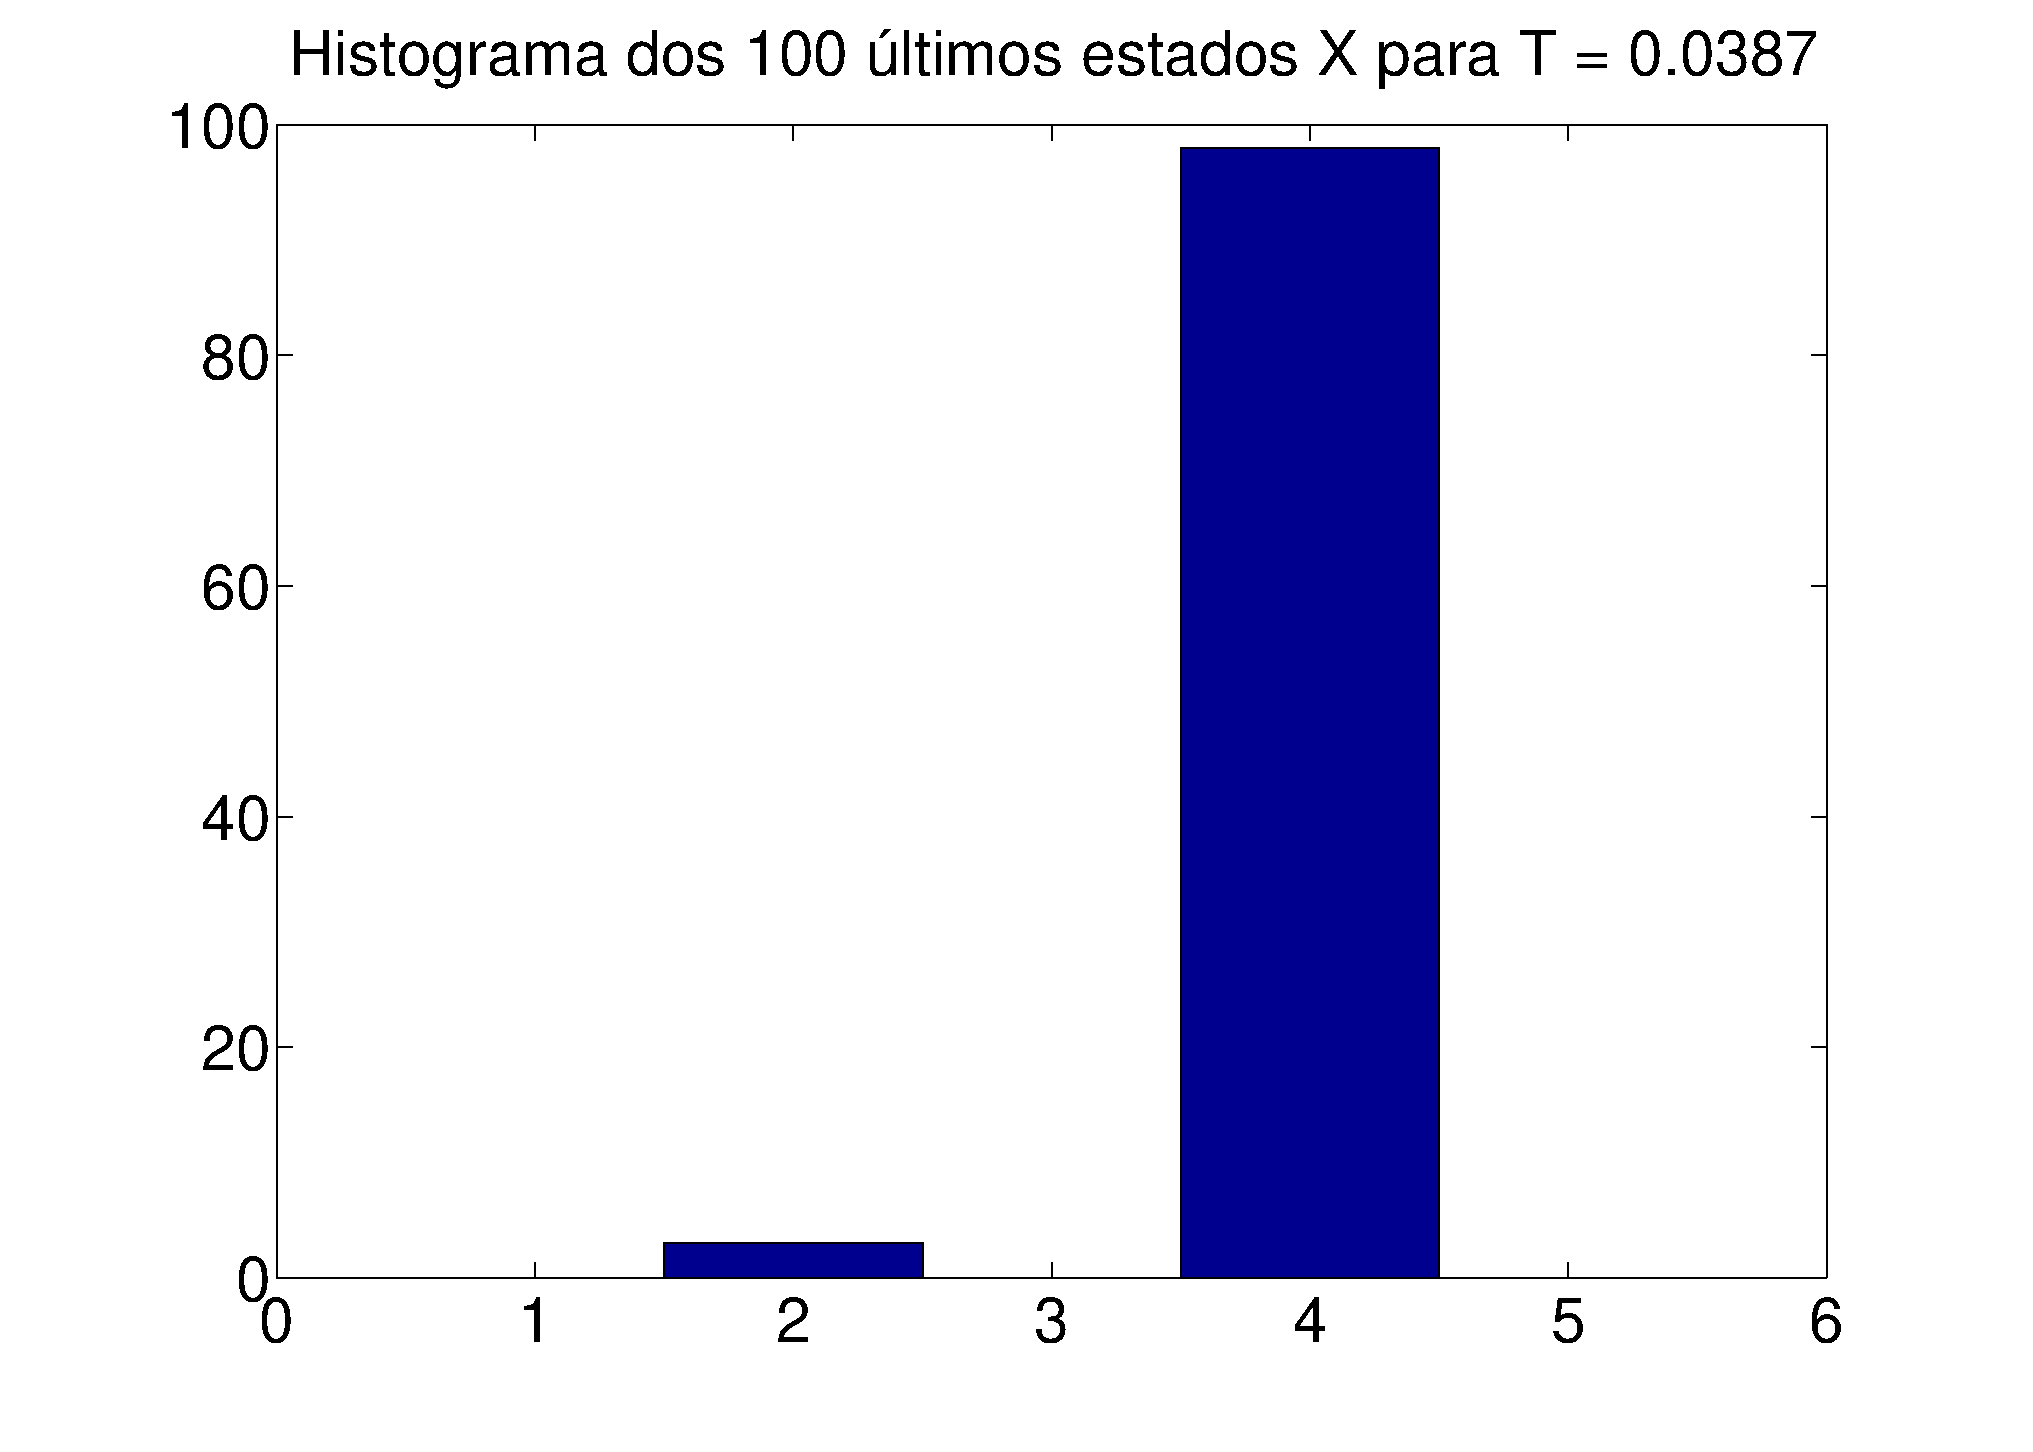
\includegraphics[width = \textwidth]{Q2_e_histograma_x_t_5}
		\caption{$T = 0.0387$}
	\end{subfigure}
		\begin{subfigure}{0.32\textwidth}
		\centering
		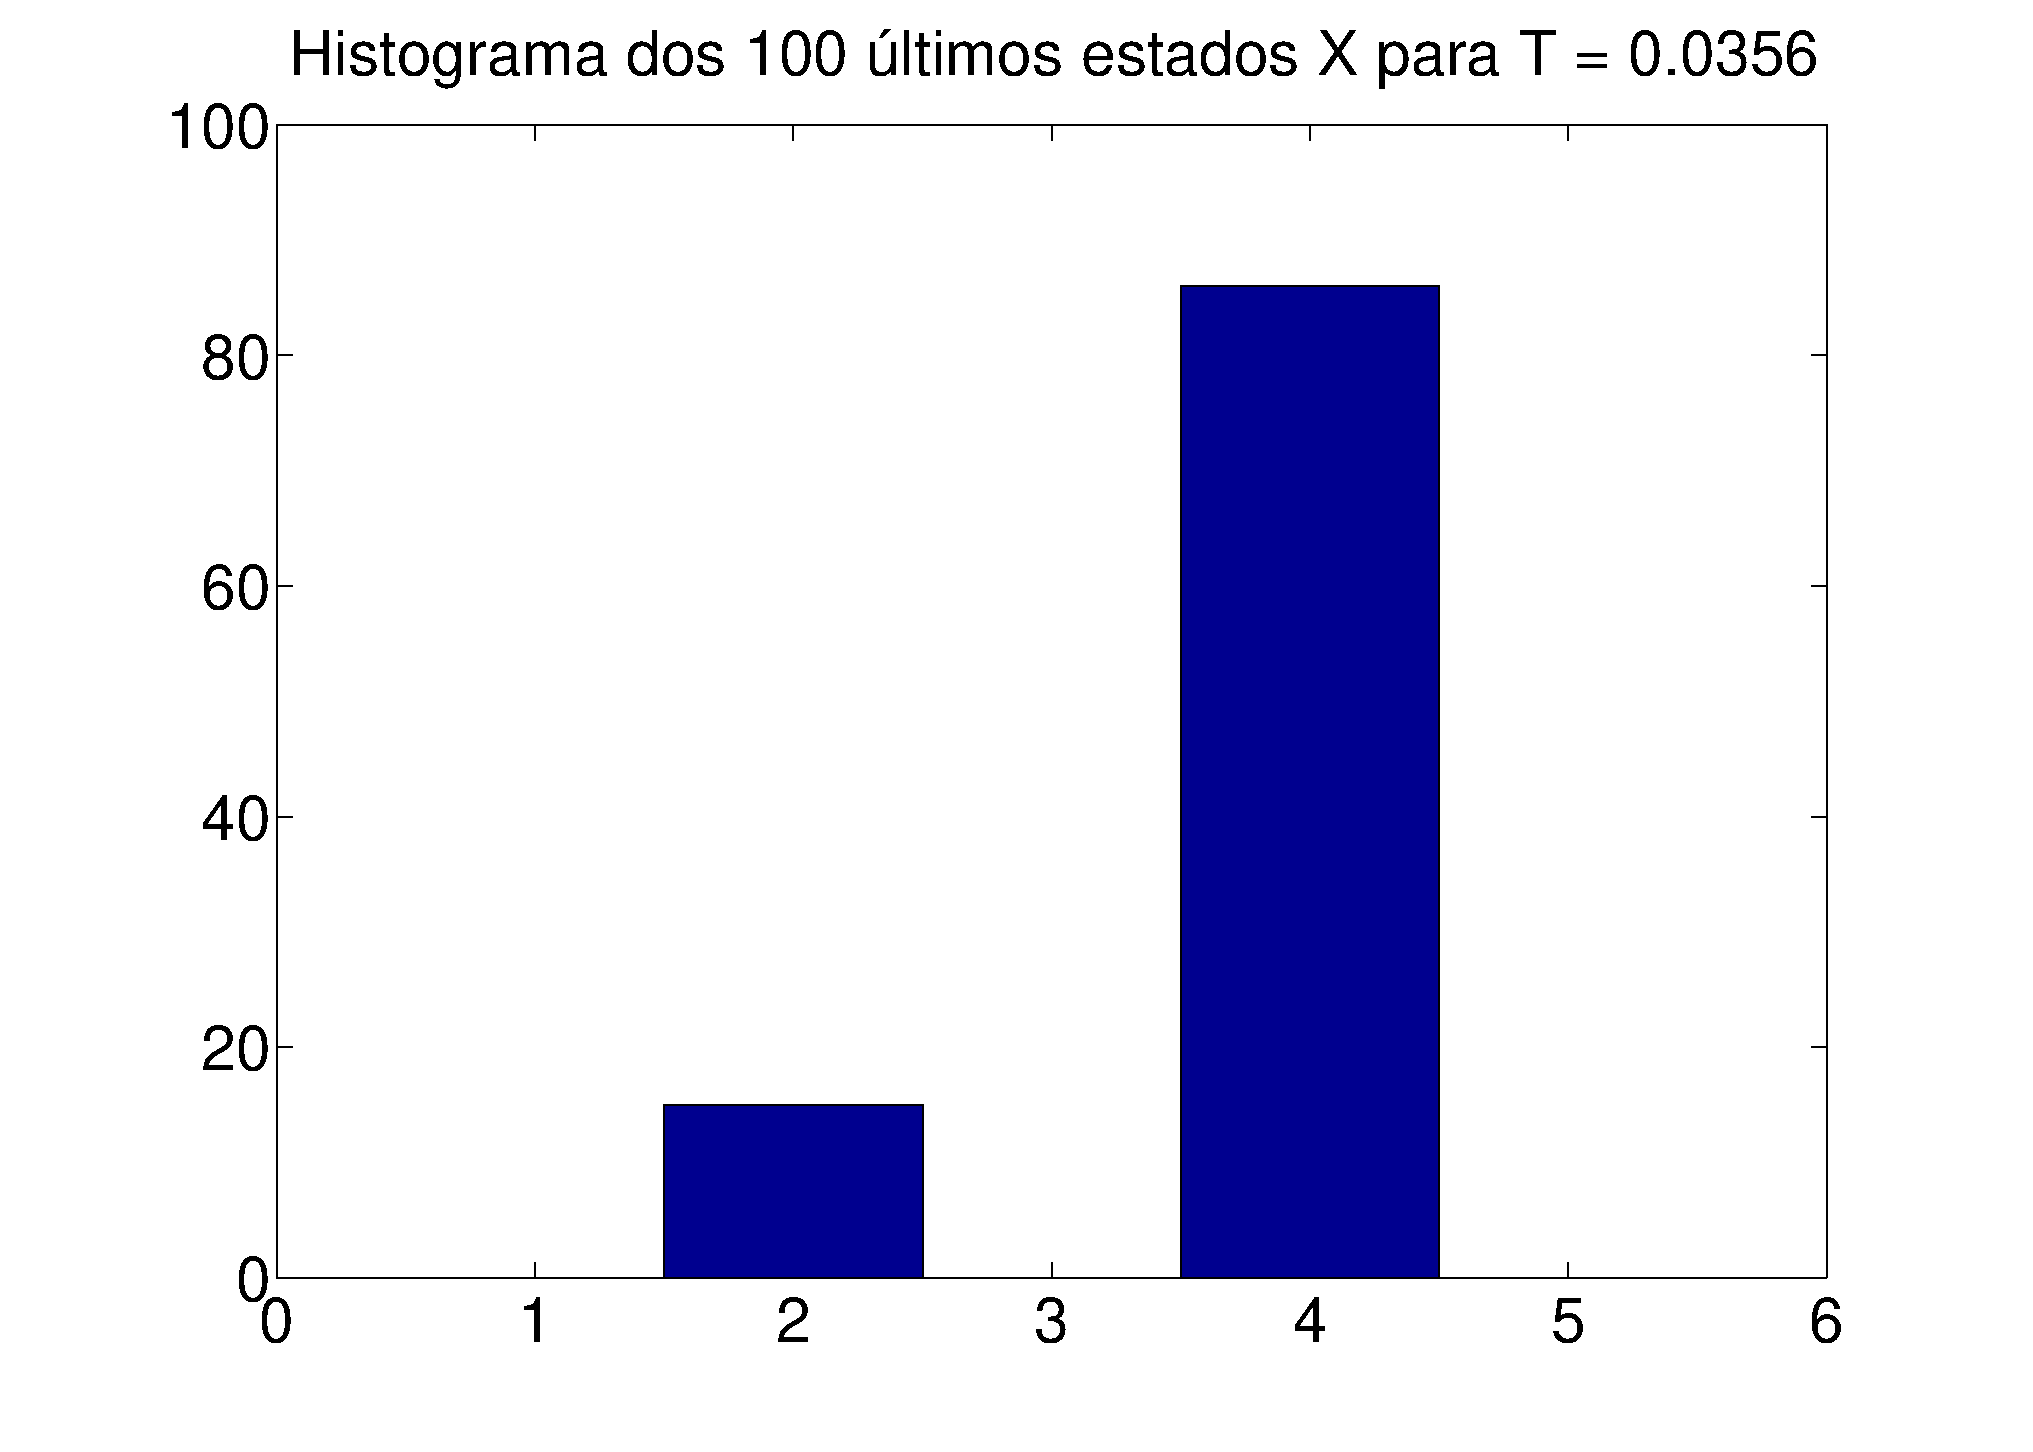
\includegraphics[width = \textwidth]{Q2_e_histograma_x_t_6}
		\caption{$T = 0.0356$}
	\end{subfigure}
		\begin{subfigure}{0.32\textwidth}
		\centering
		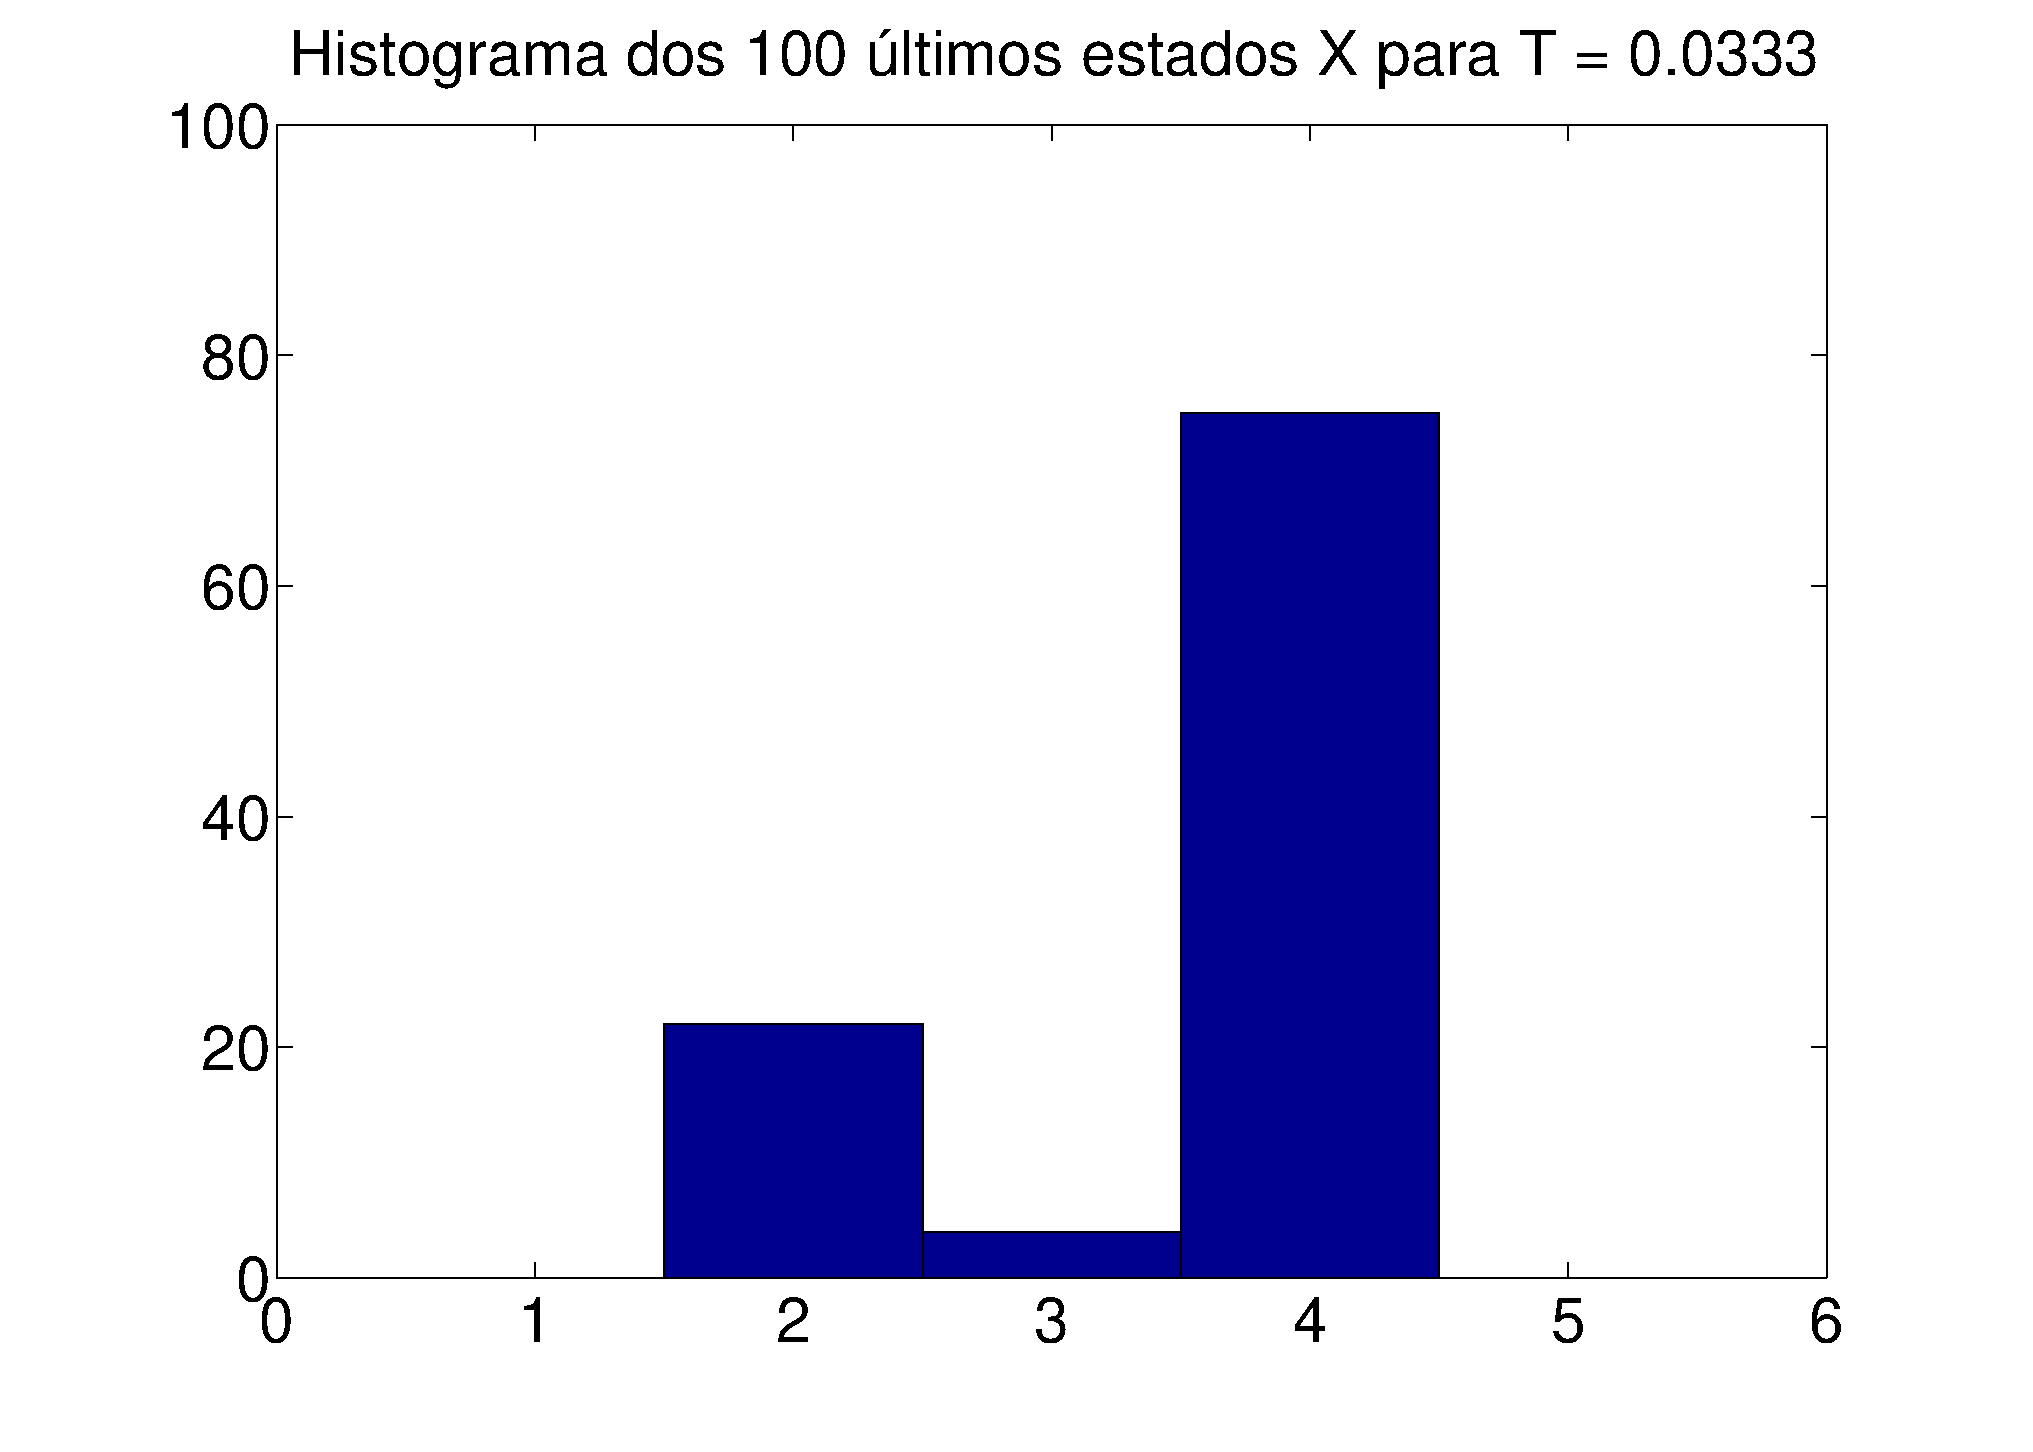
\includegraphics[width = \textwidth]{Q2_e_histograma_x_t_7}
		\caption{$T = 0.0333$}
	\end{subfigure}
		\begin{subfigure}{0.32\textwidth}
		\centering
		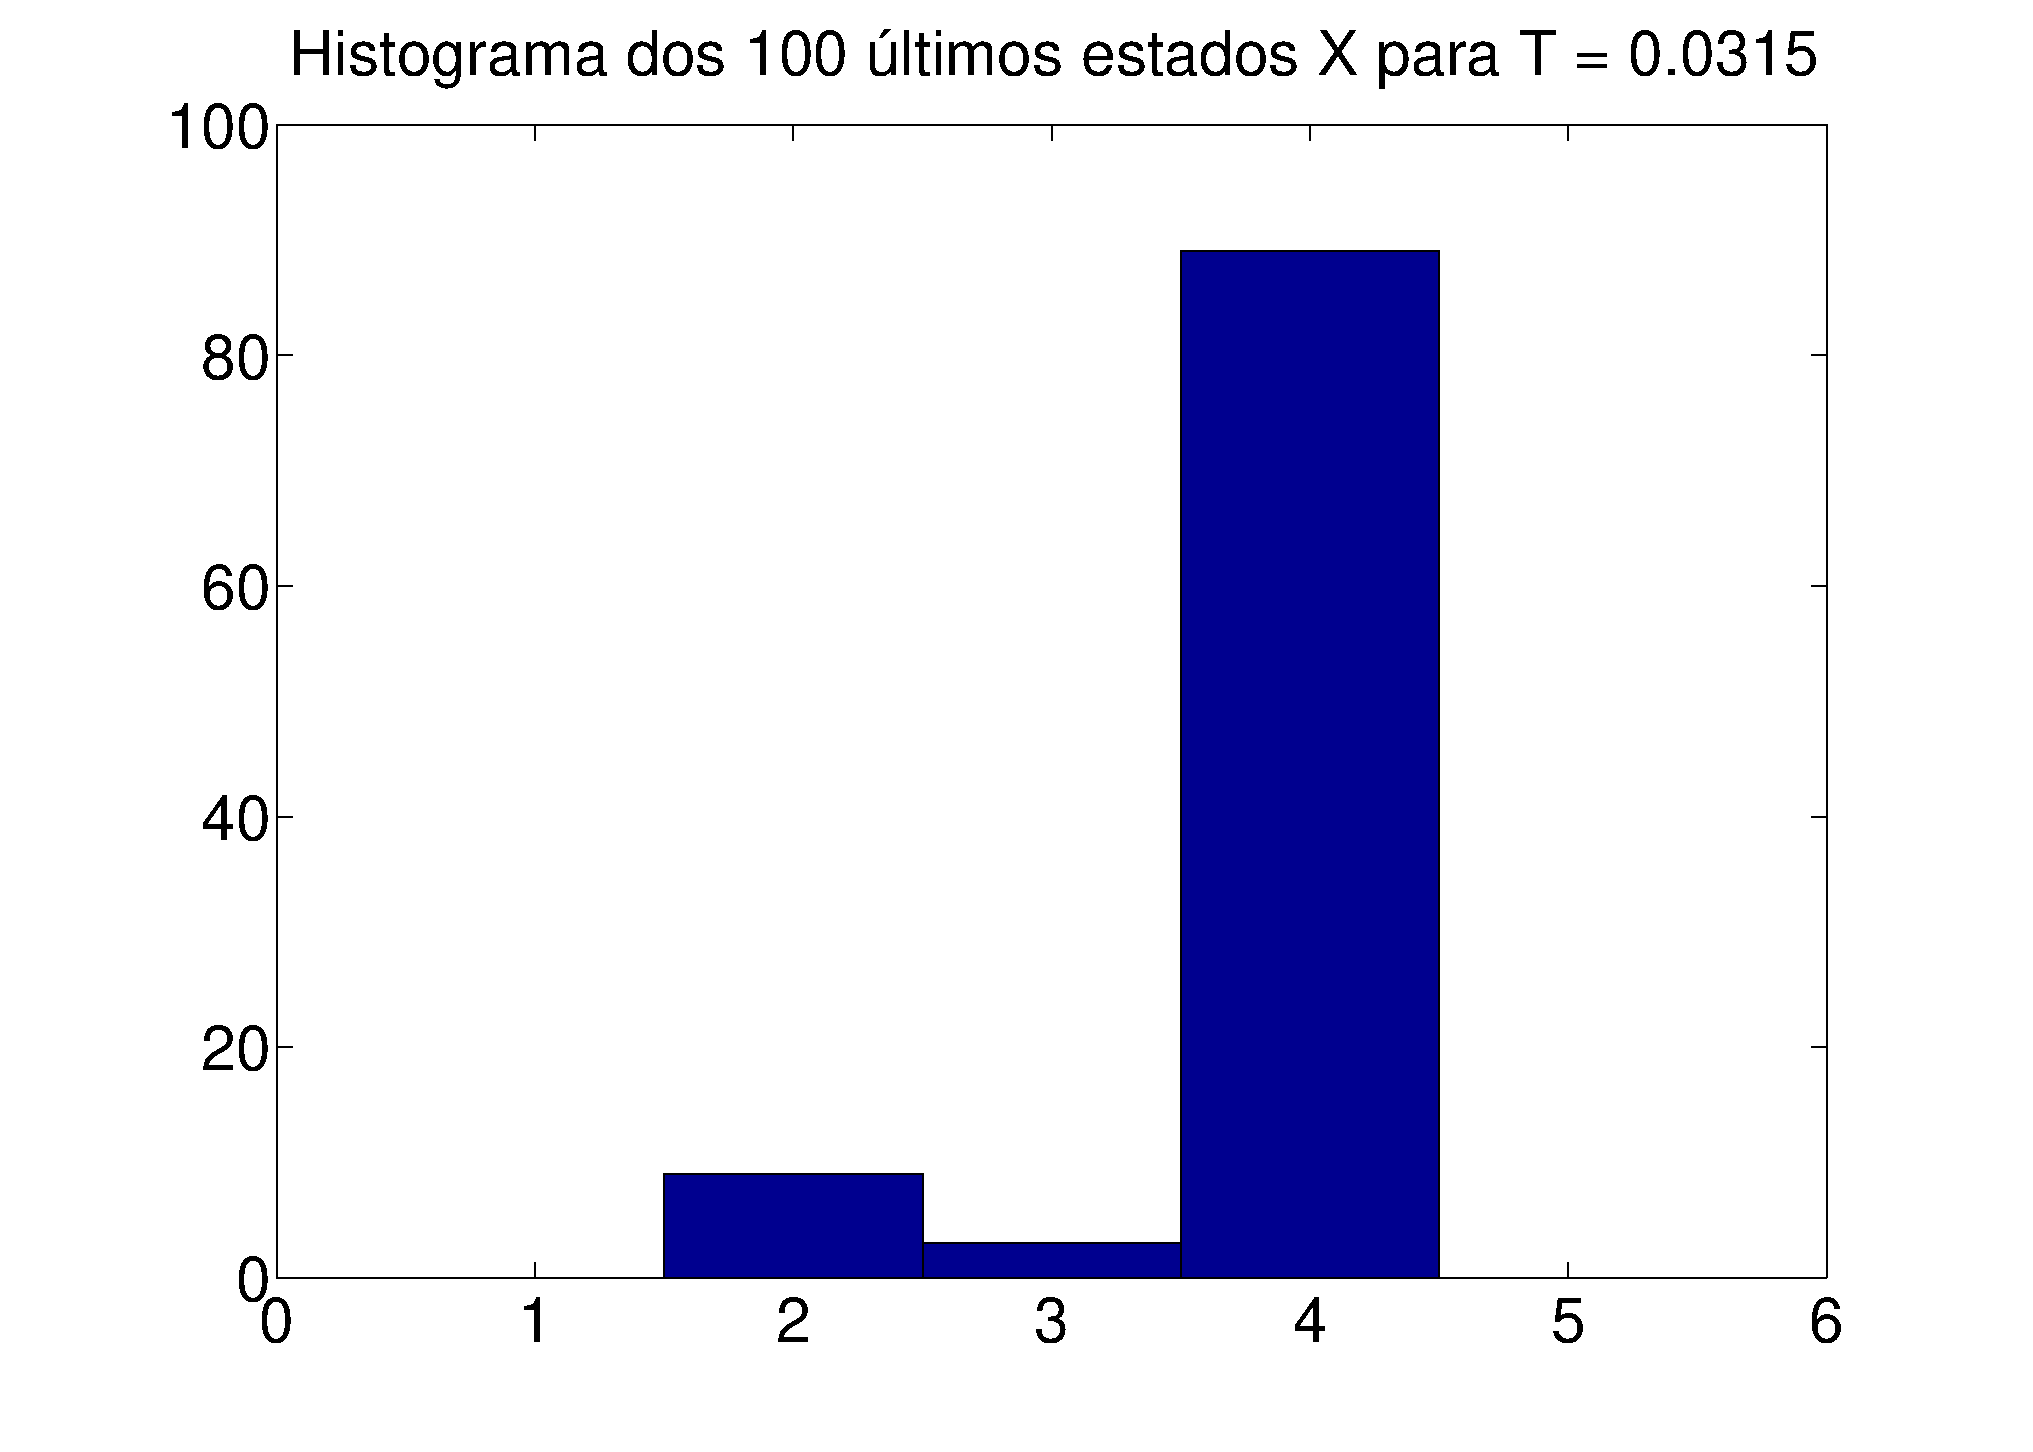
\includegraphics[width = \textwidth]{Q2_e_histograma_x_t_8}
		\caption{$T = 0.0315$}
	\end{subfigure}
		\begin{subfigure}{0.32\textwidth}
		\centering
		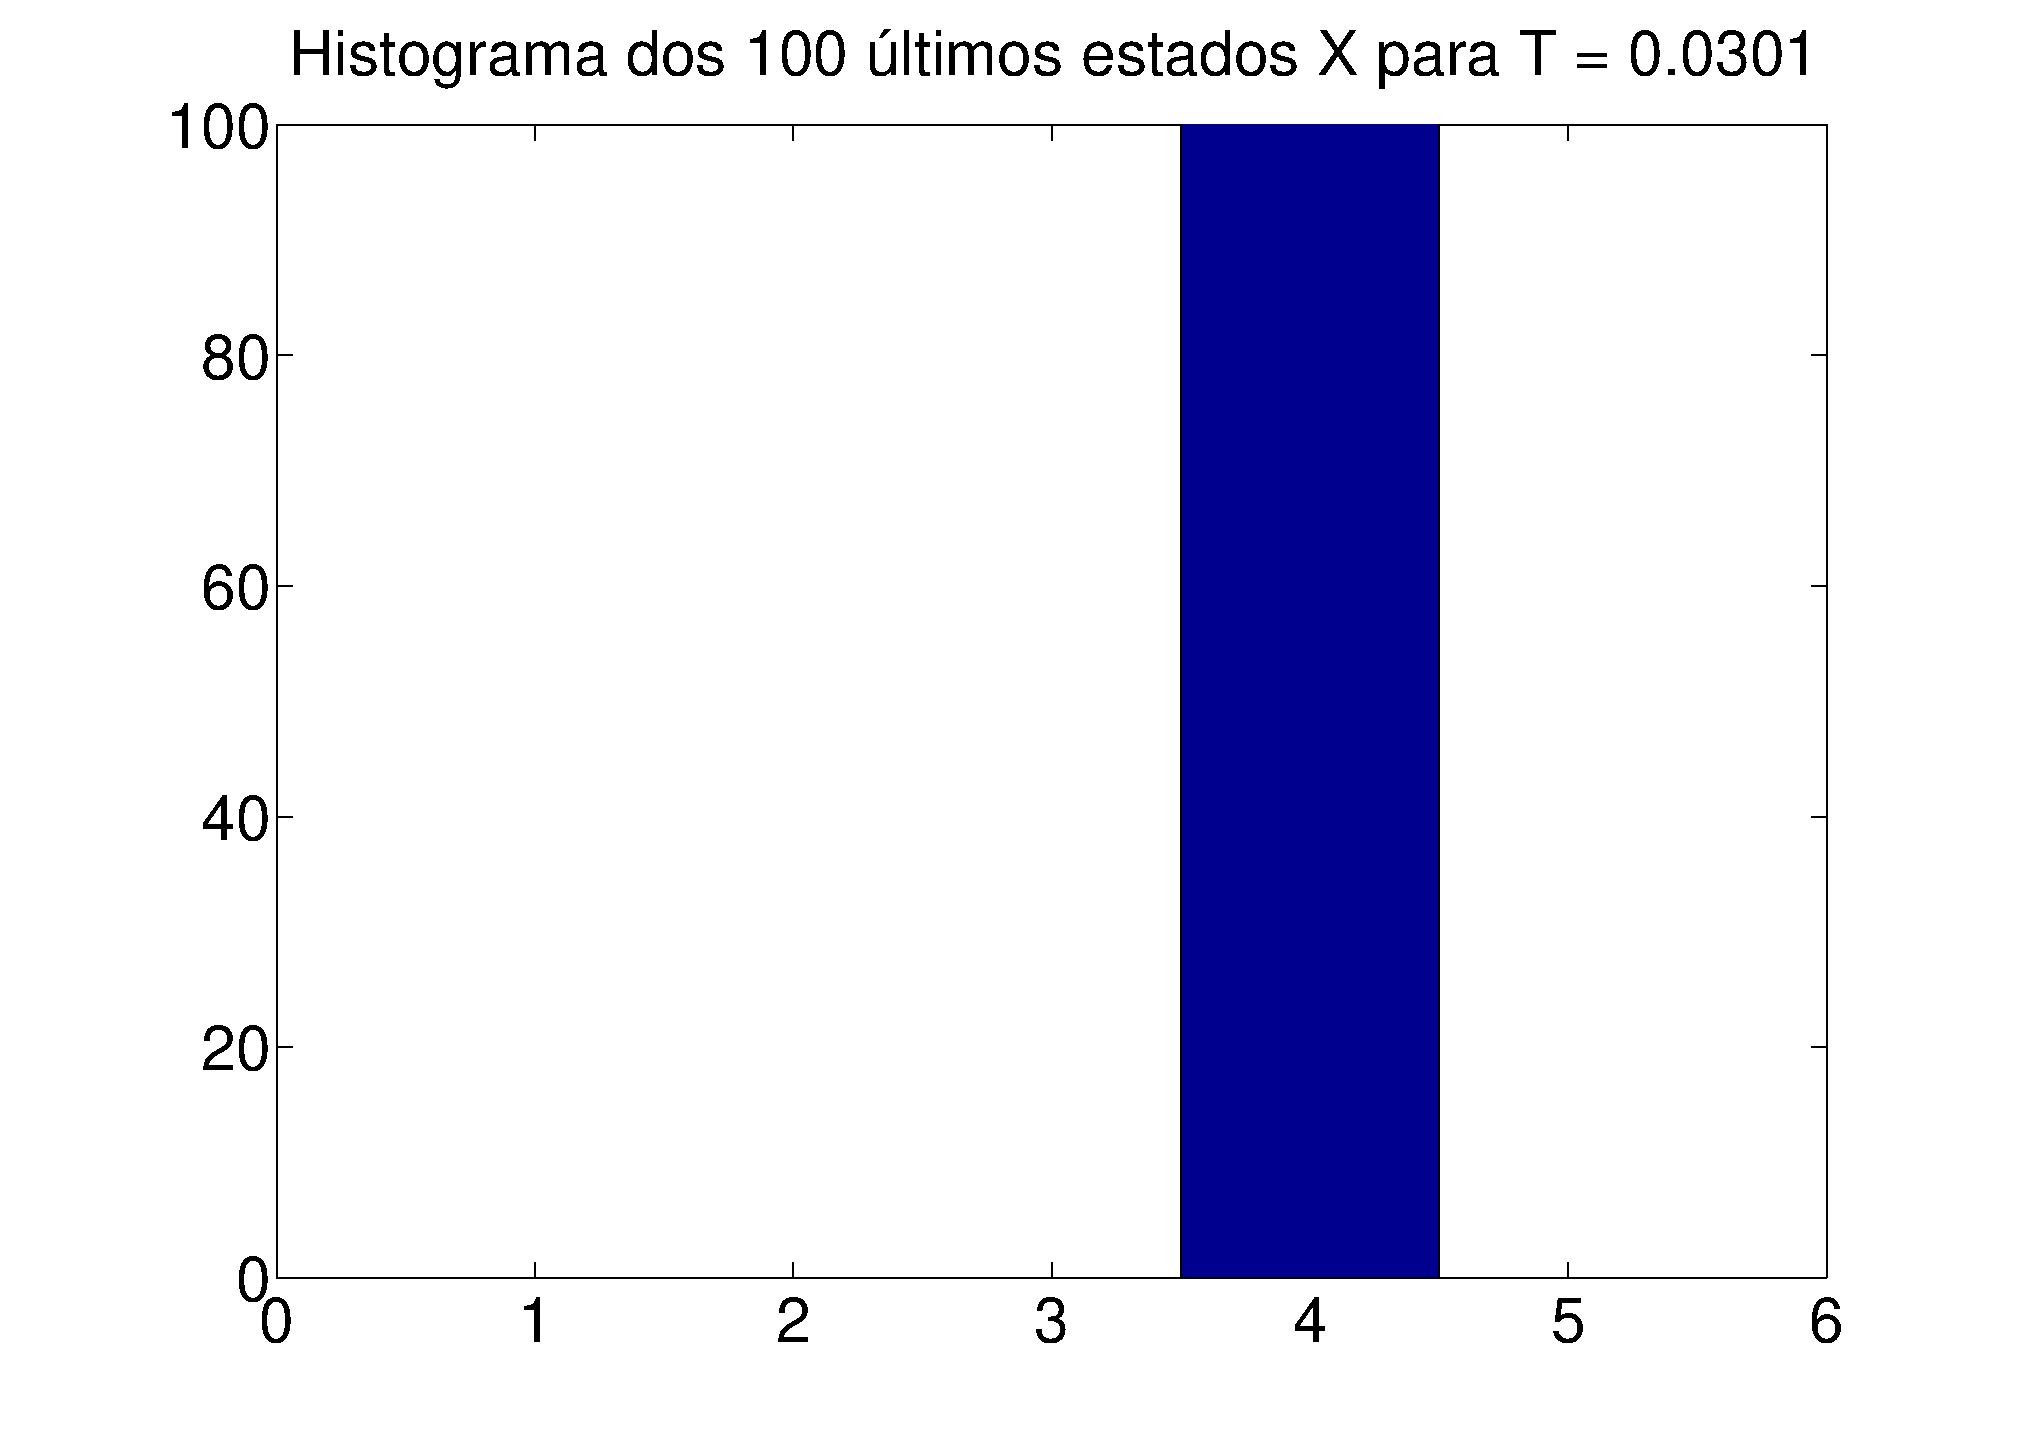
\includegraphics[width = \textwidth]{Q2_e_histograma_x_t_9}
		\caption{$T = 0.0301$}
	\end{subfigure}
		\begin{subfigure}{0.32\textwidth}
		\centering
		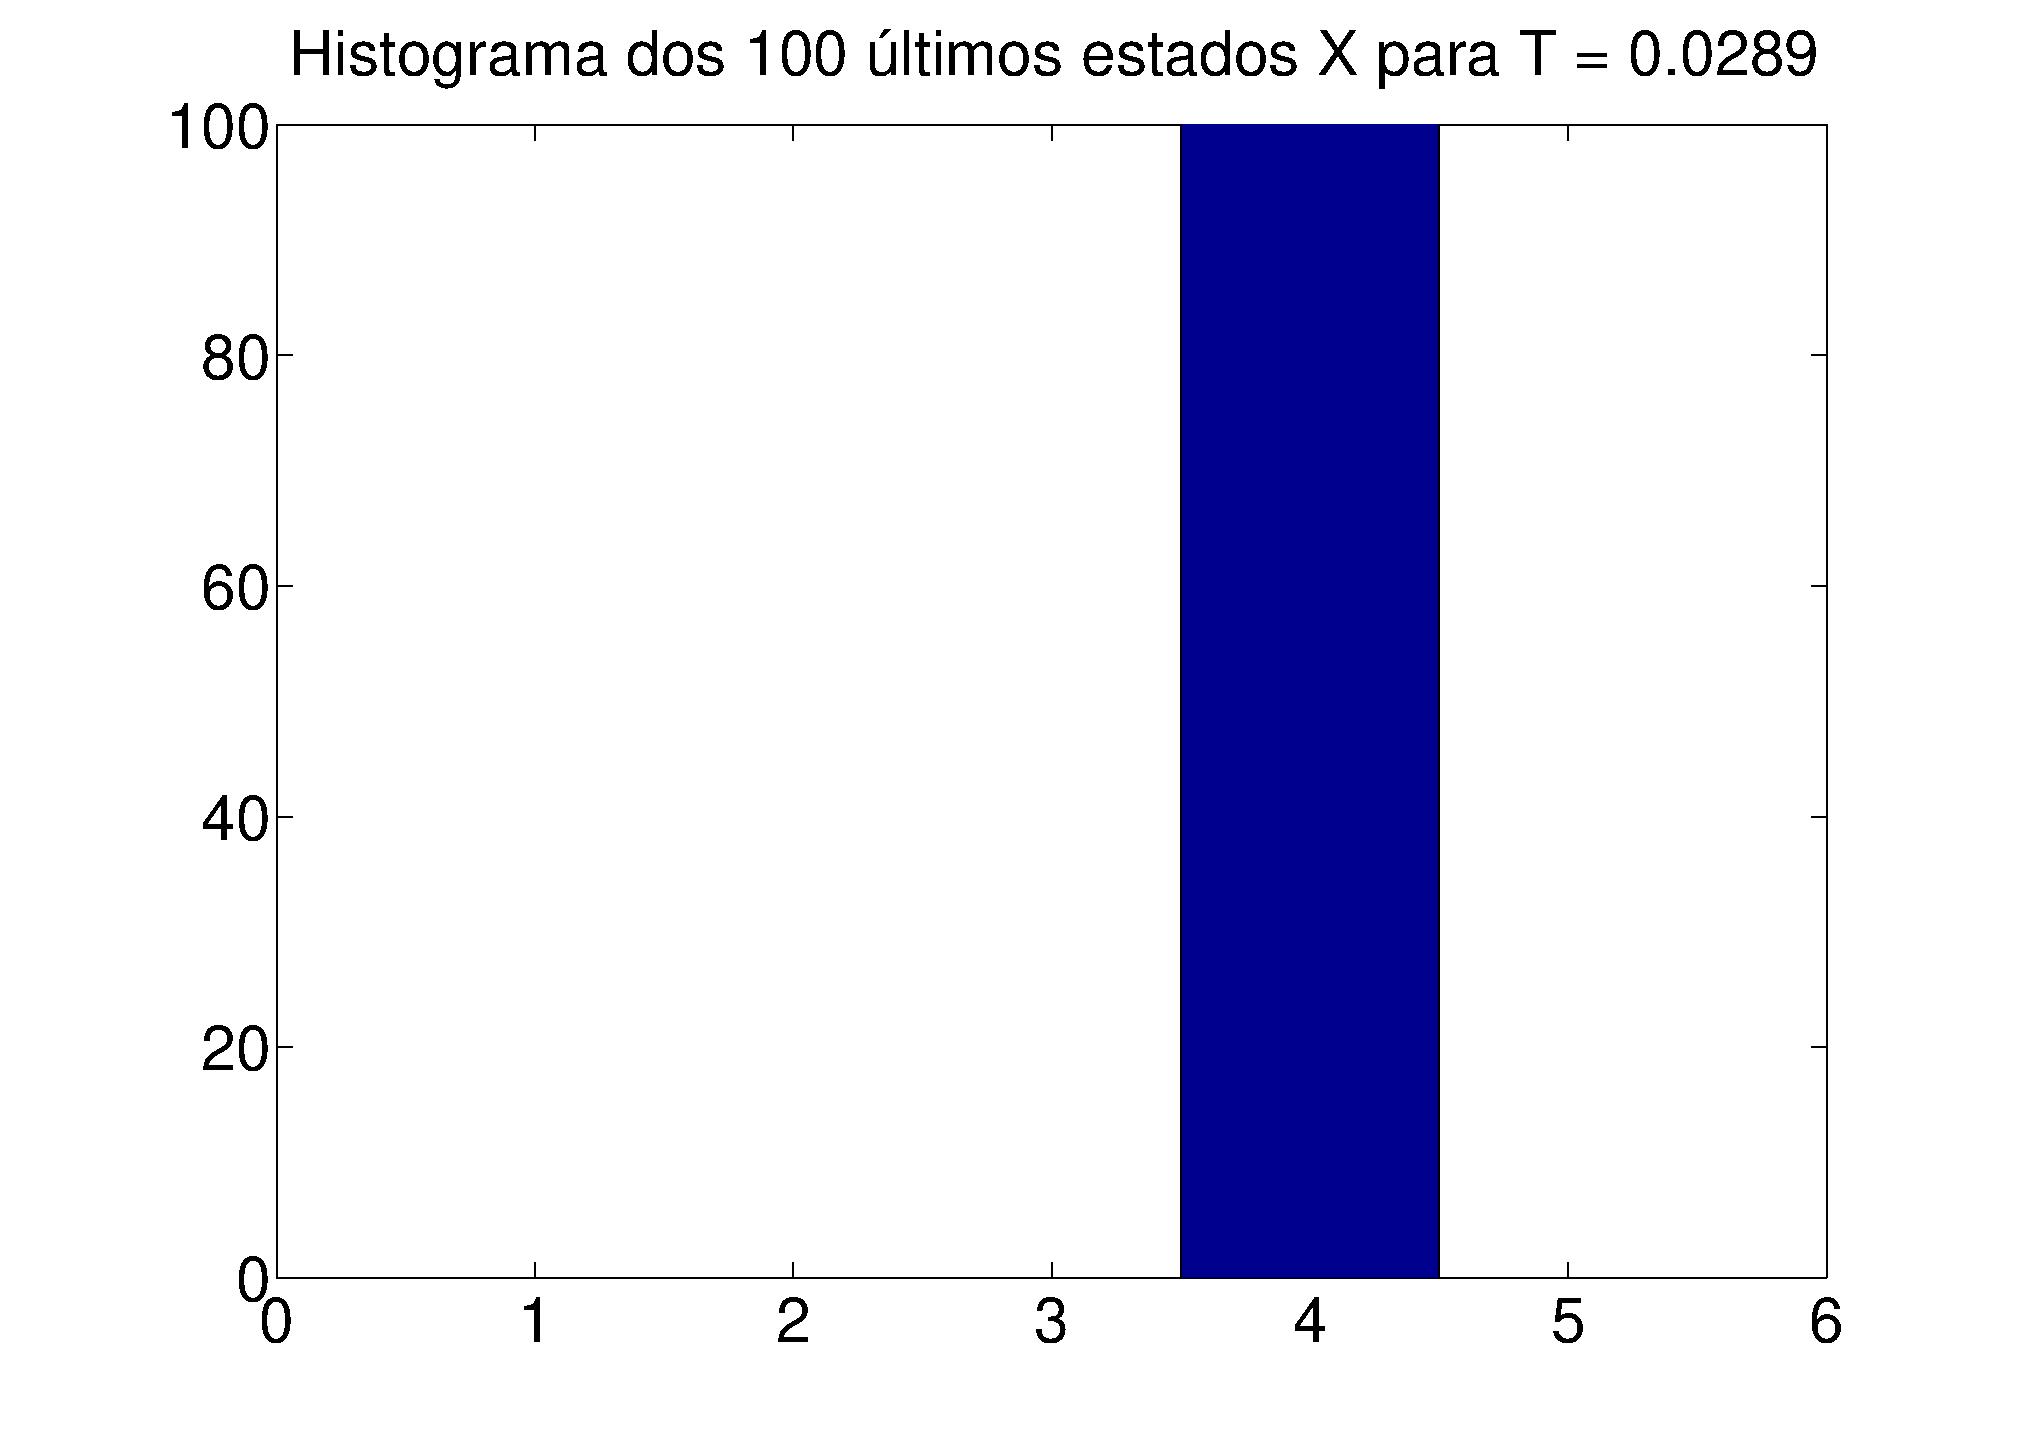
\includegraphics[width = \textwidth]{Q2_e_histograma_x_t_10}
		\caption{$T = 0.0289$}
	\end{subfigure}
	\caption{Histogramas dos últimos 100 estados de cada temperatura $T$}
	\label{histogramas_estados_temperaturas}
\end{figure}

\section*{Questão 3}

\textbf{Proponha uma função $J$(x), sendo x um vetor com 10 dimensões, cujo ponto mínimo você conheça. Evite propor funções que tenham um só ponto mínimo. Encontre o ponto mínimo global usando S.A.}\\

\textbf{Obs.: neste exercício, entregue o código utilizado e alguns comentários sobre o resultado obtido.}\\

\paragraph{} A função de custo escolhida para se minimizar é a função \emph{sync}(\textbf{x}) de 10 dimensões. Assumindo que $\mathbf{x} = [x_1 \quad x_2 \quad ... \quad x_{10}]^T$, a fórmula da \emph{sync}(\textbf{x}) é dada por:

\begin{equation*}
J(\text{\textbf{x}}) = \sum_{i=1}^{10} \sin(x_i)/x_i
\end{equation*}

\paragraph{} Por ser uma função simétrica, o mínimo global ocorre em diversos pontos. O valor mínimo dessa função é $argmin(J(\text{\textbf{x}})) \approx -2,17$. Essa função, no entanto, tende a uma superfície plana quando $x_i \rightarrow \infty, \ i = 1,2,...,10$, e isso pode fazer com que o vetor \textbf{x} se distancie cada vez mais do mínimo. De modo a evitar isso, restringe-se a região a ser considerada através da colocação de uma função $(a \times sync(\text{\textbf{x}} - \text{\textbf{b}}))^{p}$, onde \textbf{b} é um ponto no $\mathbb{R}^{10}$ sobre o qual essa função está centralizada, e $a, r > 0$ tal que eles atribuem um ganho elevado à função. Dessa forma, os estados dificilmente passarão além dessa função (assumindo que o estado inicial fique dentro da região ``delimitada" por essa função). A função custo $J(\text{\textbf{x}})$ é, portanto, dada por:\\

\begin{equation*}
J(\text{\textbf{x}}) = \sum_{i=1}^{10} \left(\sin(x_i)/x_i + (2 \times \sin(x_i - 10)/(x_i - 10))^{10}\right)
\end{equation*}

\paragraph{} O código, em MATLAB, que implementa a solução, é exibido a seguir.\\

\begin{lstlisting}
T = zeros(1,10);
T0 = 0.1;
for i = 1:10
    T(i) = T0/log2(1+i);
end

N = 10000;
epsilon = 0.1;

x_atual = random('unif', -5,5,10,1);

J_aux = sin(x_atual)./x_atual + (2*sin(x_atual - 10)./(x_atual - 10)).^10; % 'Limita' a sync(x) para valores de x entre -10 e 10
J_aux(isnan(J_aux)) = 1;
J_atual = sum(J_aux);

J_min = J_atual;

J = zeros(length(T), N);
X = zeros(size(x_atual,1),N,length(T));

for k = 1:length(T)
    for n = 1:N
        
        r = random('unif', -1,1, size(x_atual));
        
        x_futuro = x_atual + epsilon * r;
        J_aux = sin(x_futuro)./x_futuro + (2*sin(x_futuro - 10)./(x_futuro - 10)).^10; 
        J_aux(isnan(J_aux)) = 1;
        J_futuro = sum(J_aux);
        
        delta_J = J_futuro - J_atual;
        
        if delta_J < 0
            x_atual = x_futuro;
            J_atual = J_futuro;
        else
            a = rand();
            
            if a < exp(-(delta_J)/T(k))
                x_atual = x_futuro;
                J_atual = J_futuro;
            end
        end
        
        if J_atual < J_min
            J_min = J_atual;
            X_min = x_atual;
        end
        
        J(k,n) = J_atual;
        X(:,n,k) = x_atual;
        
    end
end

% Resultados
% 
% J_min =
% 
%    -2.1542
%    
% X_min =
% 
%    -4.3440
%     4.3660
%     4.2649
%    -4.5078
%    -4.5456
%     4.5105
%     4.6312
%    -4.3770
%     4.5351
%    -4.6876   
\end{lstlisting}

\paragraph{} O valor mínimo encontrado é bem próximo do mínimo global da função, apontado anteriormente. Como se observa pelos histogramas dos valores de J para diferentes temperaturas, exibidos na Figura \ref{histogramas_custos_temperaturas_v2}, conforme se diminui a temperatura, mais o histograma vai se concentrando próximo ao valor mínimo da função.

\begin{figure}[H]
	\centering
	\begin{subfigure}{0.3\textwidth}
		\centering
		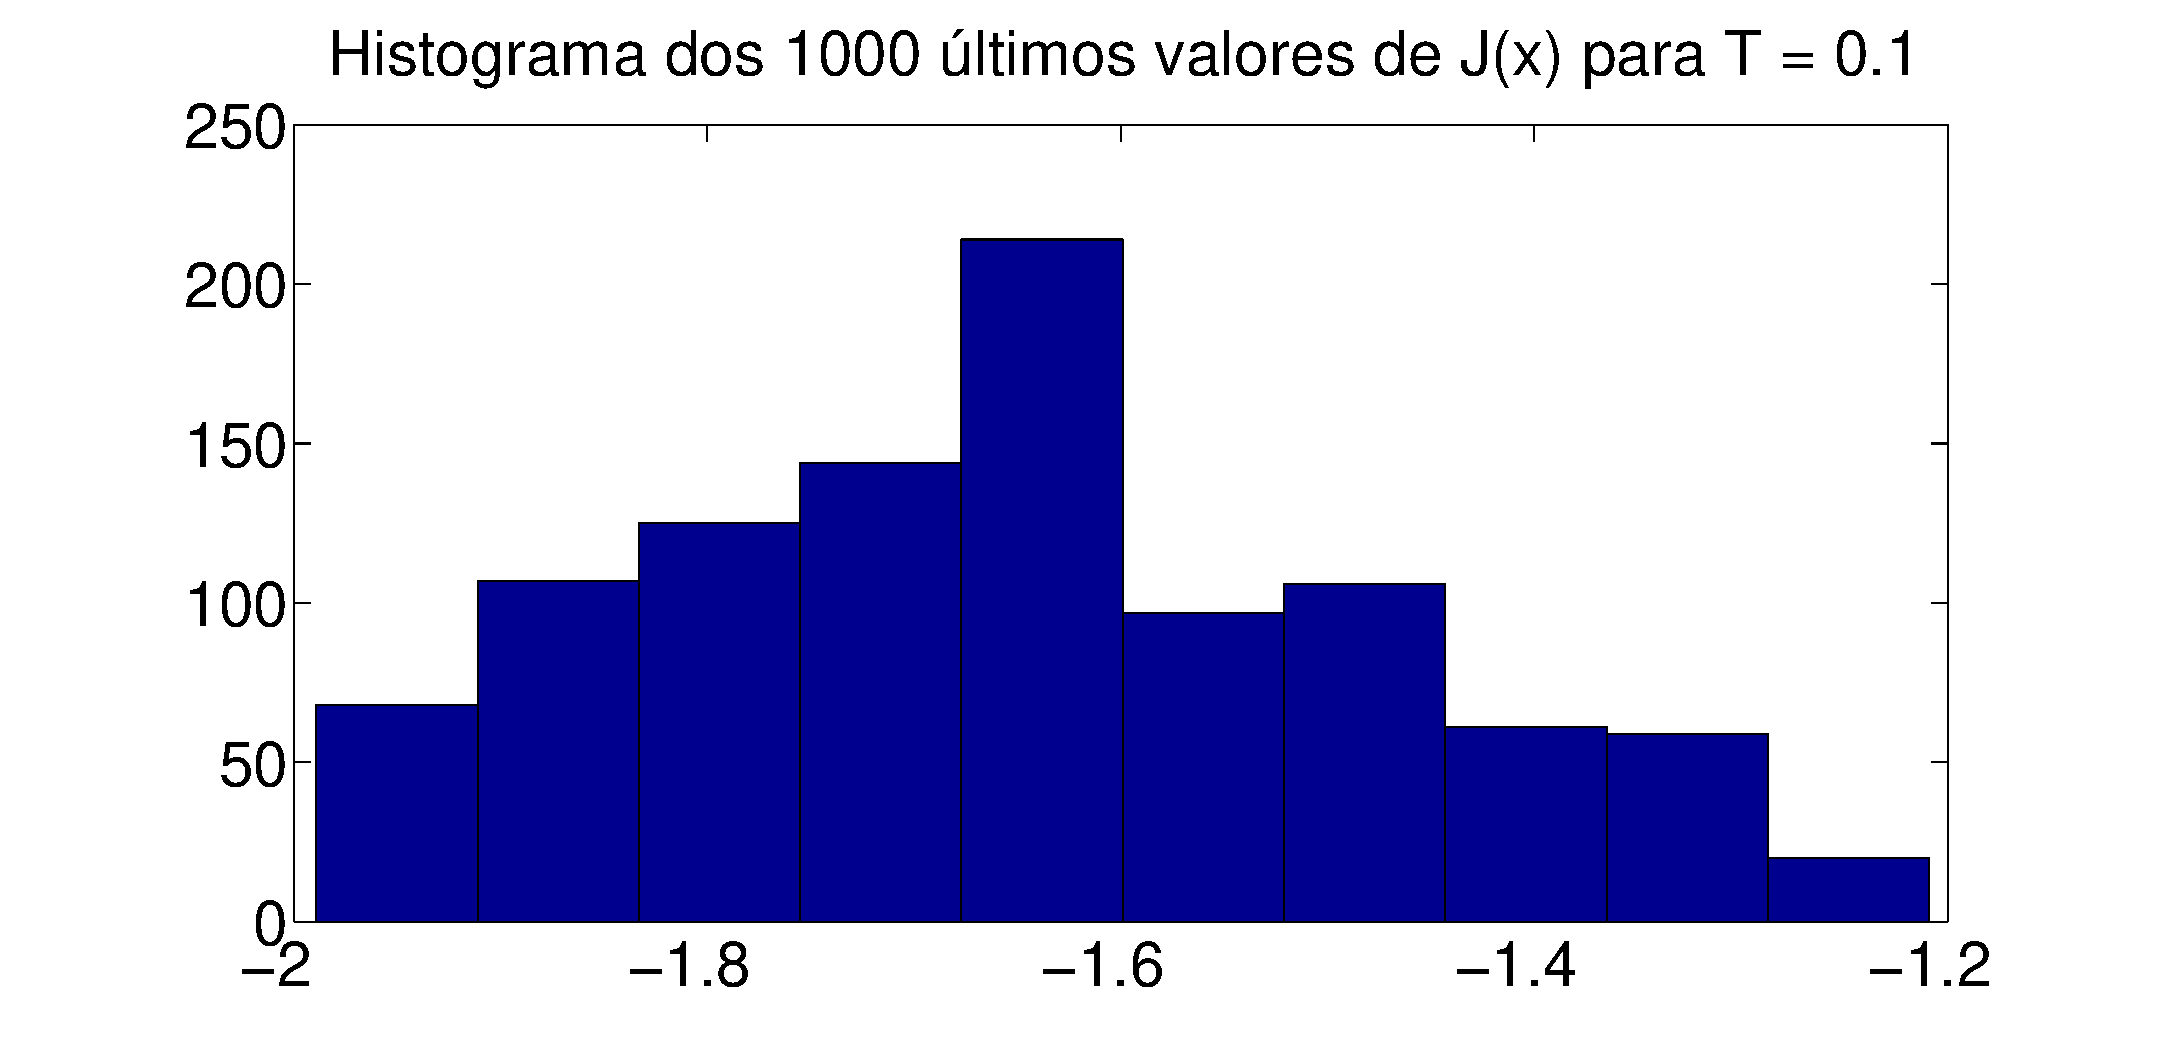
\includegraphics[width = \textwidth]{Q3_histograma_J_t_1_v2}
		\caption{$T = 0.1$}
	\end{subfigure}
	\begin{subfigure}{0.3\textwidth}
		\centering
		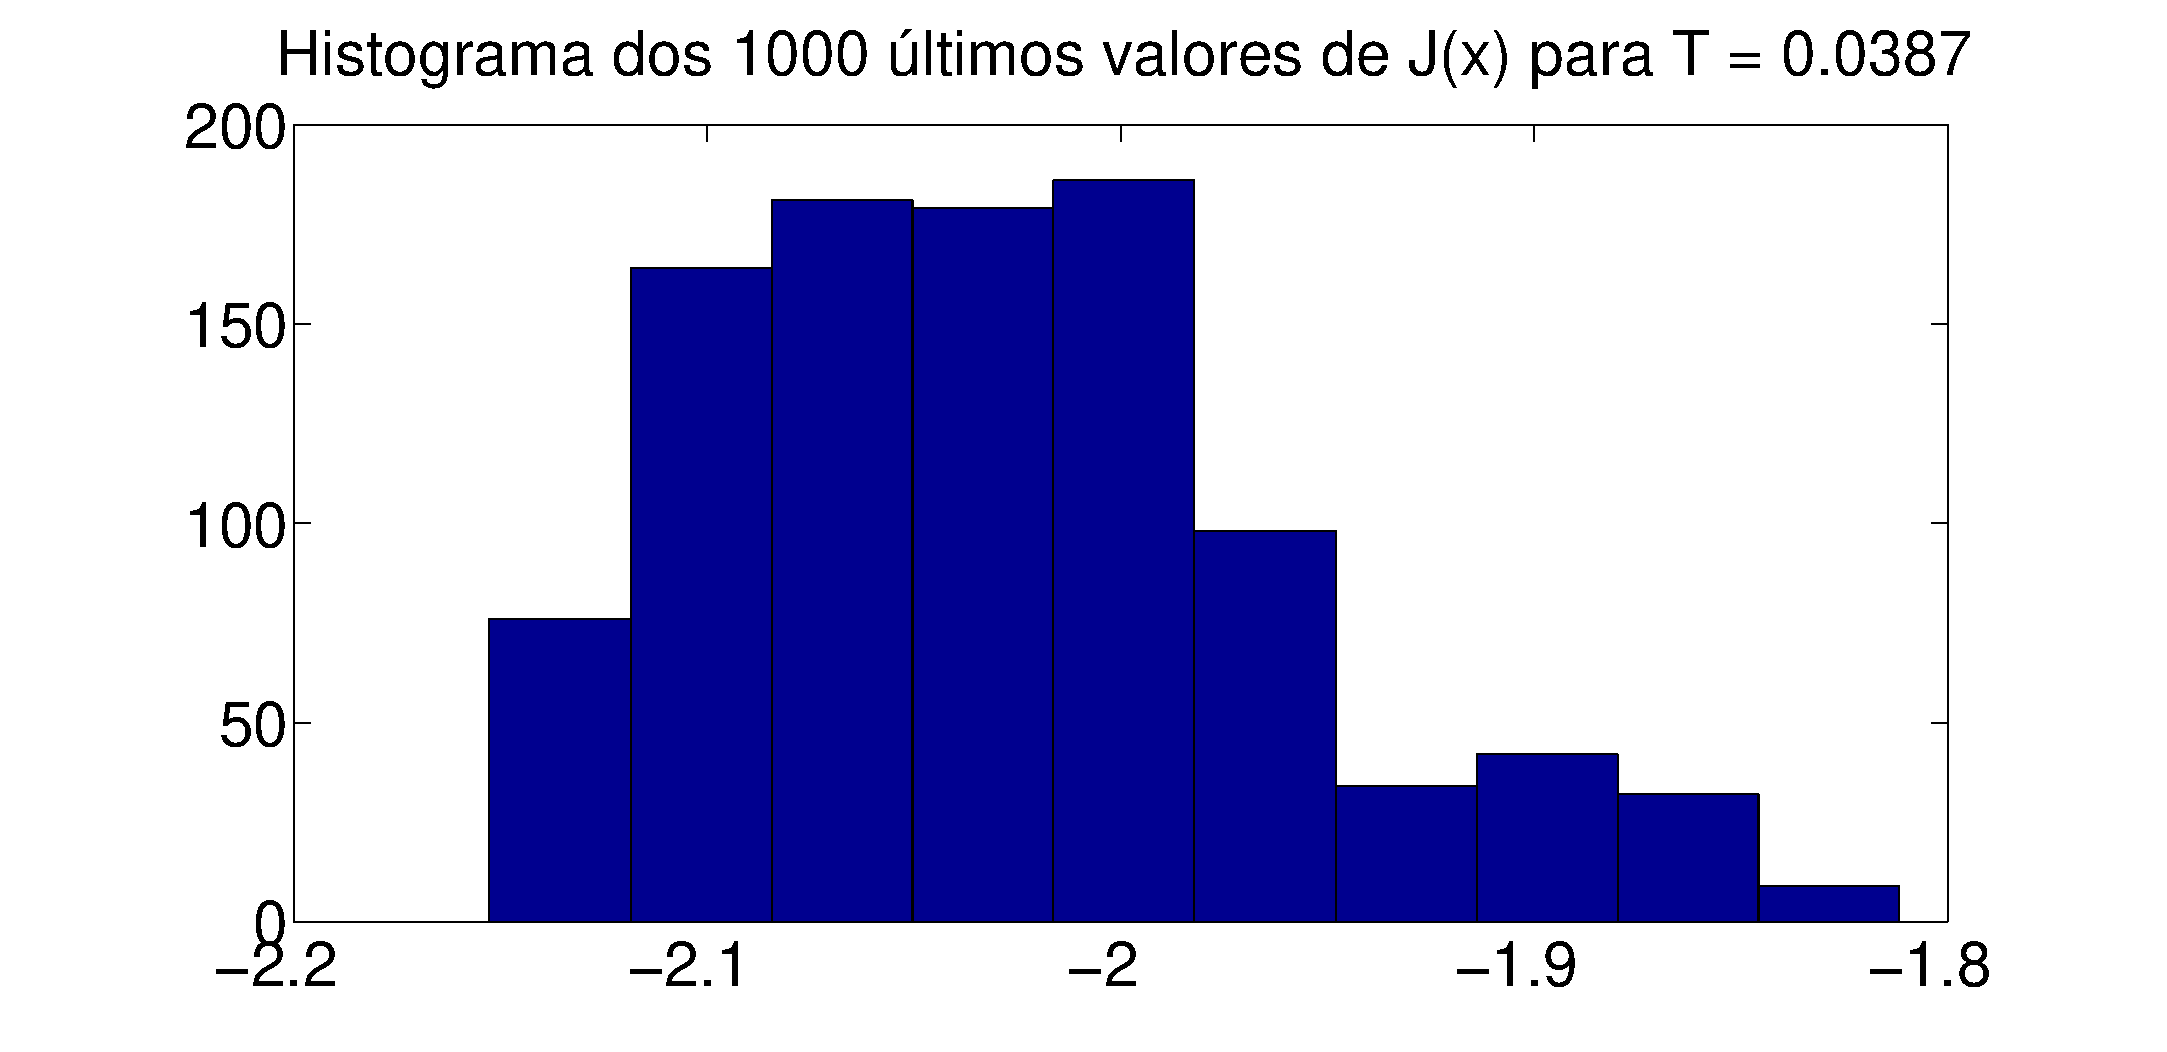
\includegraphics[width = \textwidth]{Q3_histograma_J_t_5_v2}
		\caption{$T = 0.0387$}
	\end{subfigure}
	\begin{subfigure}{0.3\textwidth}
		\centering
		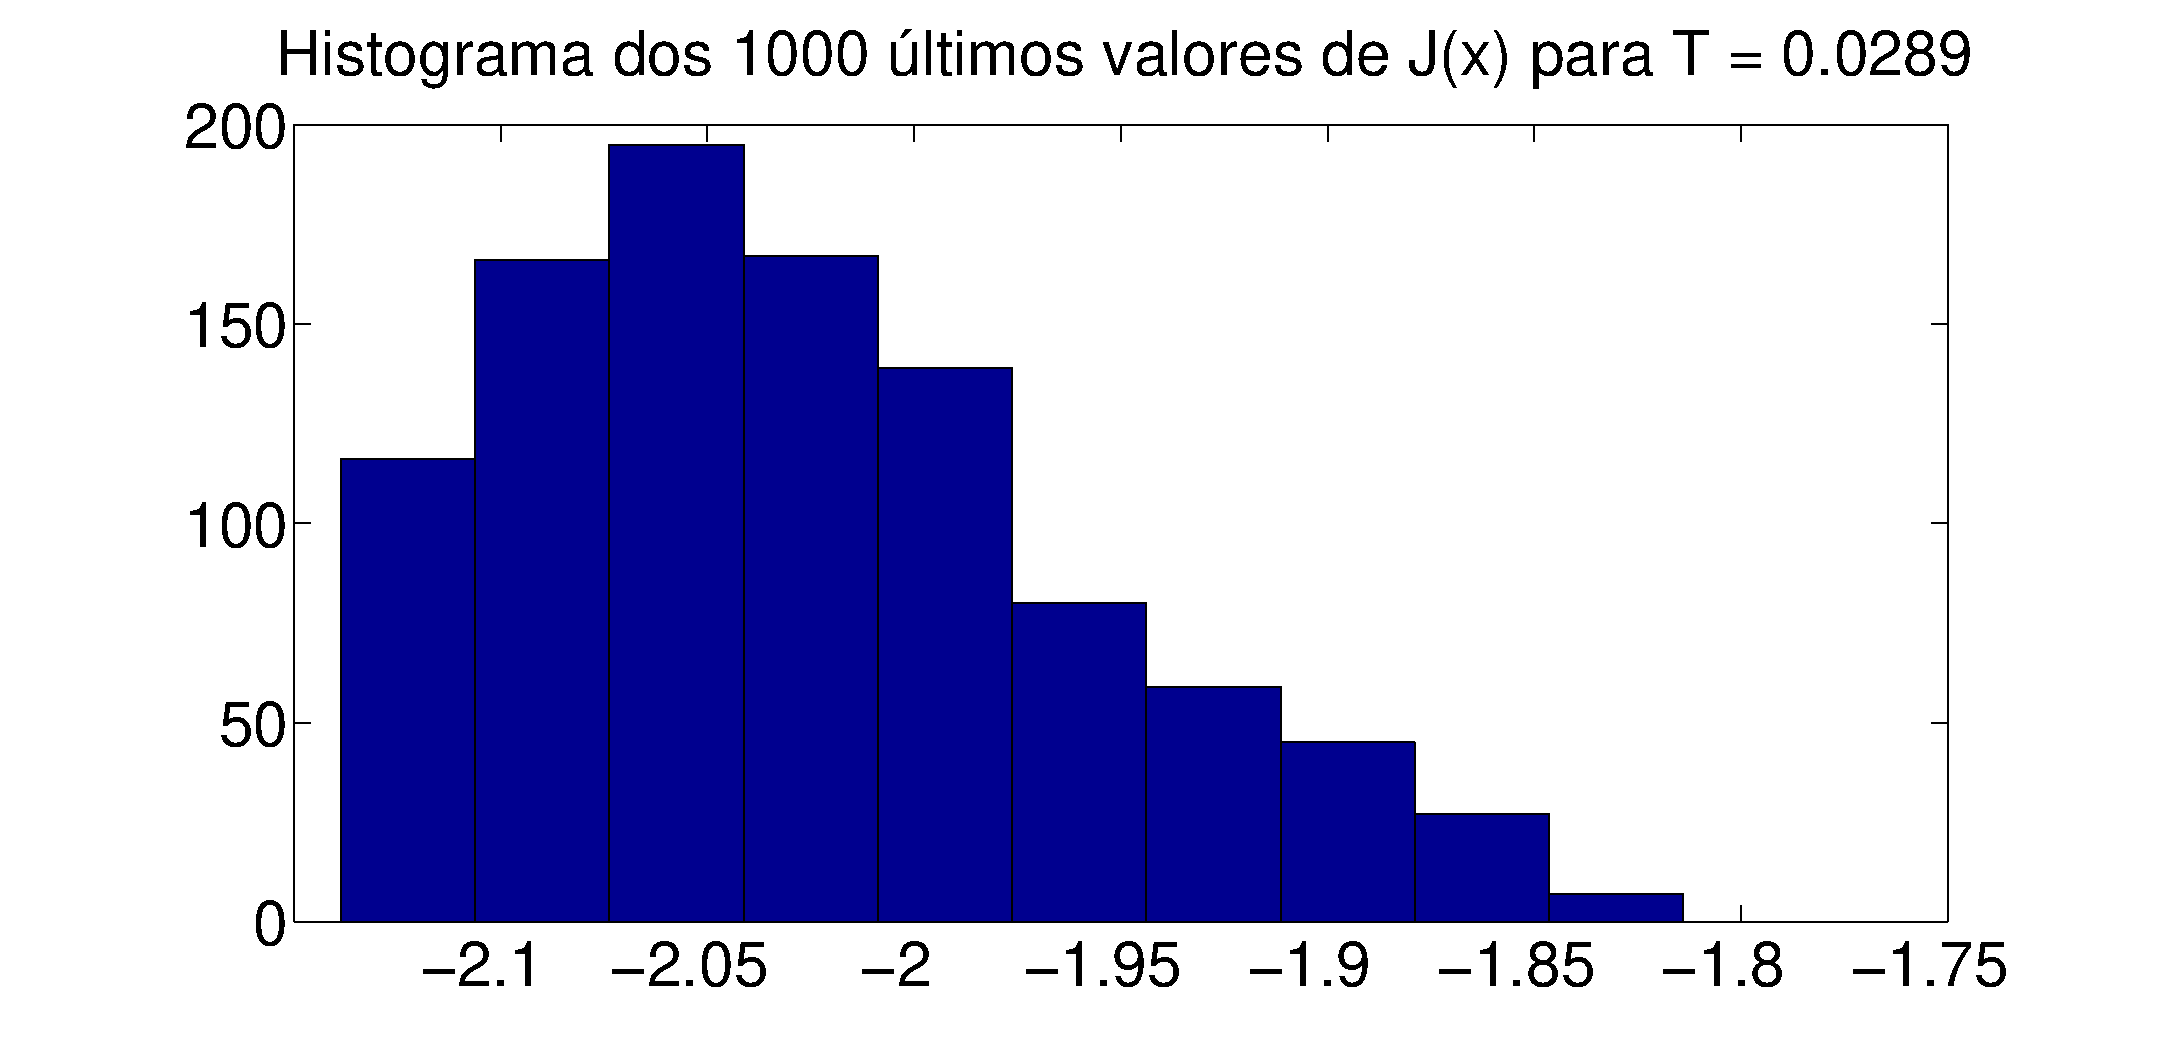
\includegraphics[width = \textwidth]{Q3_histograma_J_t_10_v2}
		\caption{$T = 0.0289$}
	\end{subfigure}
	\caption{Histogramas de valores da função $J(\text{\textbf{x}})$ para diferentes temperaturas.}
	\label{histogramas_custos_temperaturas_v2}
\end{figure}

\begin{comment}

\paragraph{} Assumindo que $\mathbf{x} = [x_1 \quad x_2 \quad ... \quad x_{10}]^T$, a função que se escolheu minimizar é dada por:\\

\begin{equation*}
J(\text{\textbf{x}}) = \sum_{i=1}^{10} x_i^2
\end{equation*}

\paragraph{} O código, em MATLAB, que implementa a solução, é exibido a seguir.\\

\begin{lstlisting}
T = zeros(1,20);
T0 = 0.1;
for i = 1:20
    T(i) = T0/log2(1+i);
end
x_atual = random('unif', -5,5,10,1);
J_atual = sum(x_atual.^2);

J_min = J_atual;
N = 10000;
epsilon = 0.1;

J = zeros(length(T), N);
X = zeros(size(x_atual,1), N, length(T));

for k = 1:length(T)
    for n = 1:N
        
        r = random('unif',-1,1,size(x_atual));
        x_futuro = x_atual + epsilon * r;
        
        J_futuro = sum(x_futuro.^2);
        
        delta_J = J_futuro - J_atual;
        
        if delta_J < 0
            x_atual = x_futuro;
            J_atual = J_futuro;
            
        else
            a = rand();
            
            if a < exp(-(delta_J)/T(k))
                x_atual = x_futuro;
                J_atual = J_futuro;
            end
        end
        
       if J_atual < J_min
           J_min = J_atual;
           X_min = x_atual;
       end
        
       J(k, n) = J_atual;
       X(:,n,k) = x_atual;
    end
           
end

% Resultados:
% 
% J_min =
% 
%     0.0075
%     
% X_min =
% 
%     0.0245
%     0.0190
%     0.0210
%    -0.0458
%     0.0146
%     0.0163
%    -0.0092
%    -0.0528
%    -0.0259
%     0.0022
\end{lstlisting}

\paragraph{} O valor mínimo encontrado é, de fato, próximo do mínimo global da função, o qual é $0$. Como se observa pelos histogramas dos valores de J para diferentes temperaturas, exibidos na Figura \ref{histogramas_custos_temperaturas}, conforme se diminui a temperatura, mais o histograma vai se concentrando próximo ao valor mínimo da função. No código, utilizou-se 20 temperaturas, com resfriamento logarítmico. A Figura \ref{histogramas_custos_temperaturas} exibe os histogramas da temperatura inicial ($T = 0.5$), intermediária ($T = 0.1445$) e final ($T = 0.1138$).\\ 

\begin{figure}[H]
	\centering
	\begin{subfigure}{0.3\textwidth}
		\centering
		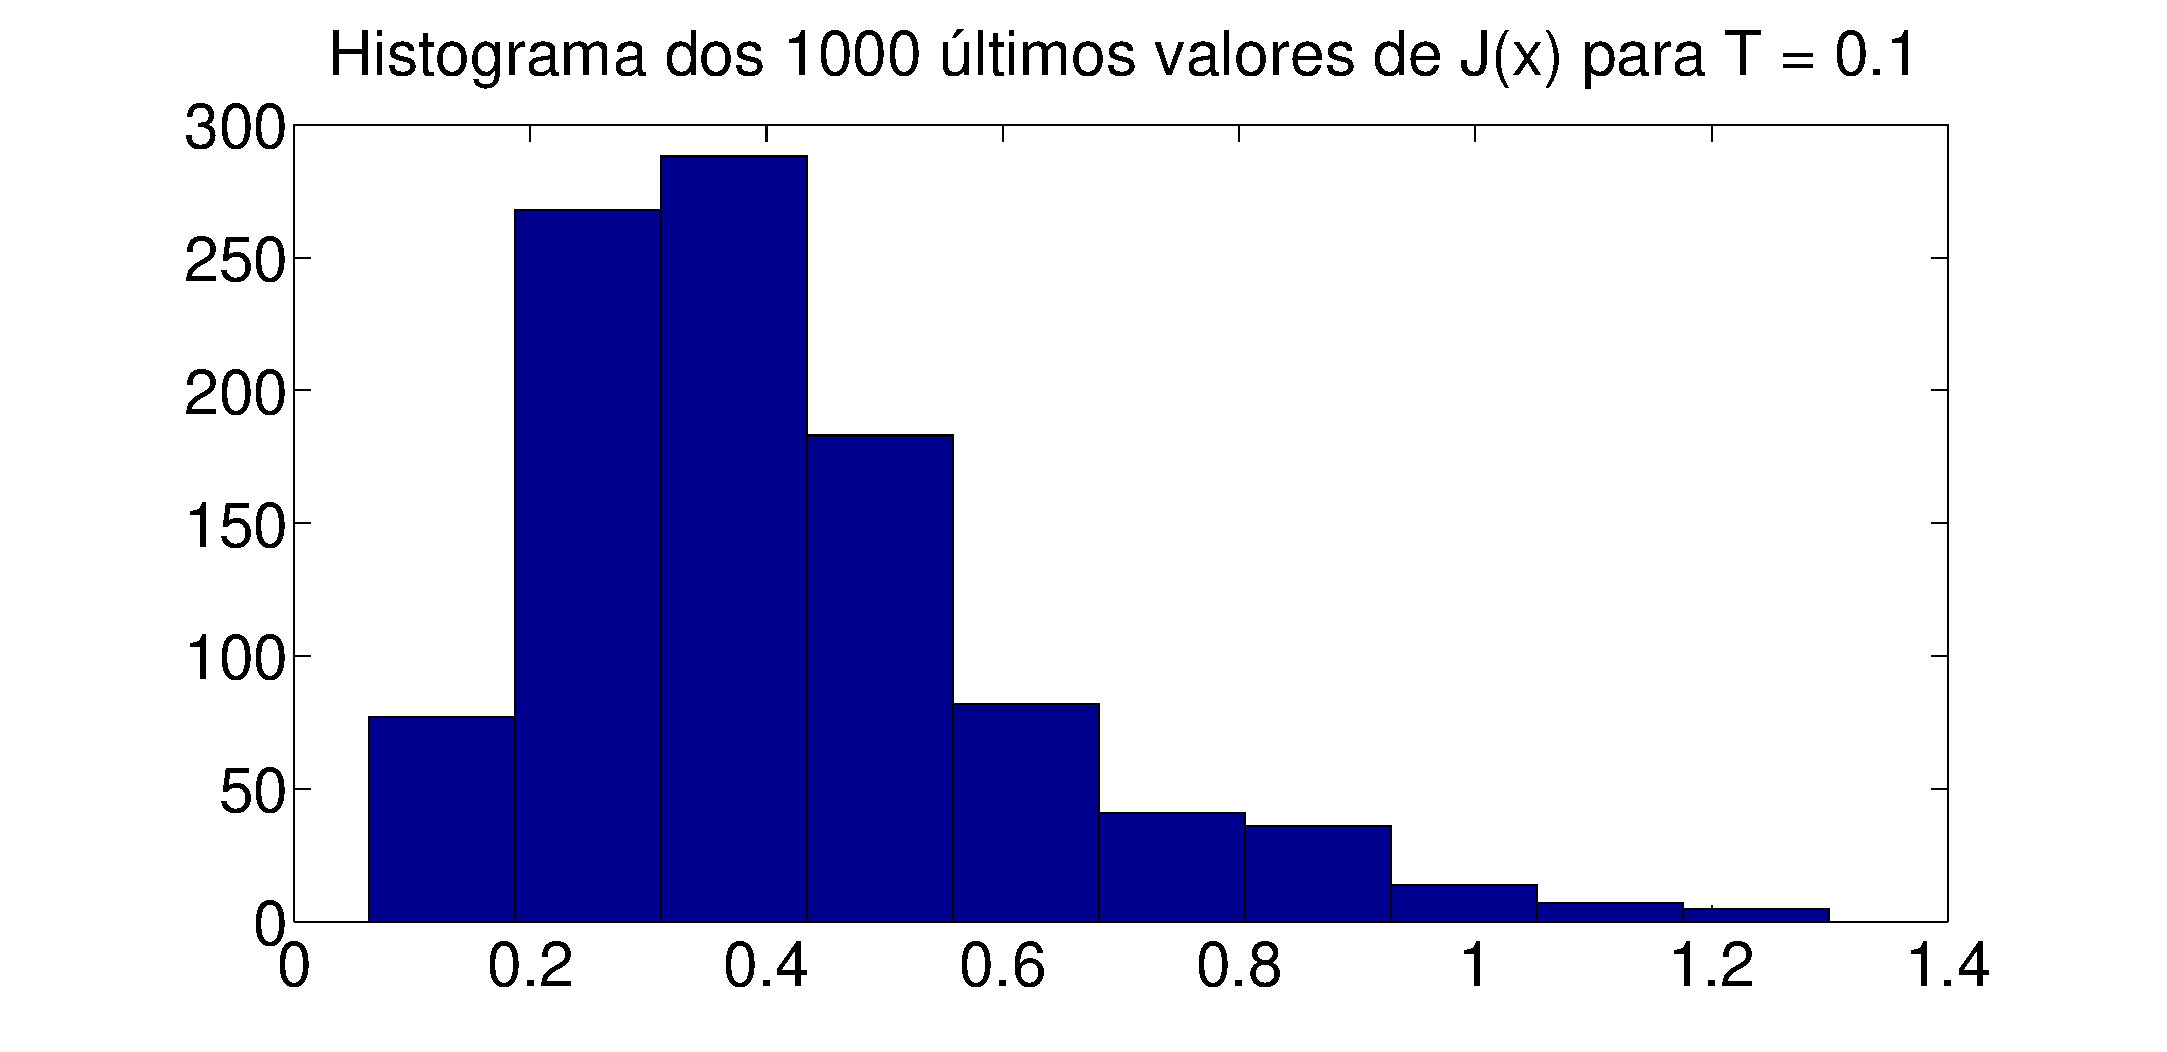
\includegraphics[width = \textwidth]{Q3_histograma_J_t_1}
		\caption{$T = 0.1$}
	\end{subfigure}
	\begin{subfigure}{0.3\textwidth}
		\centering
		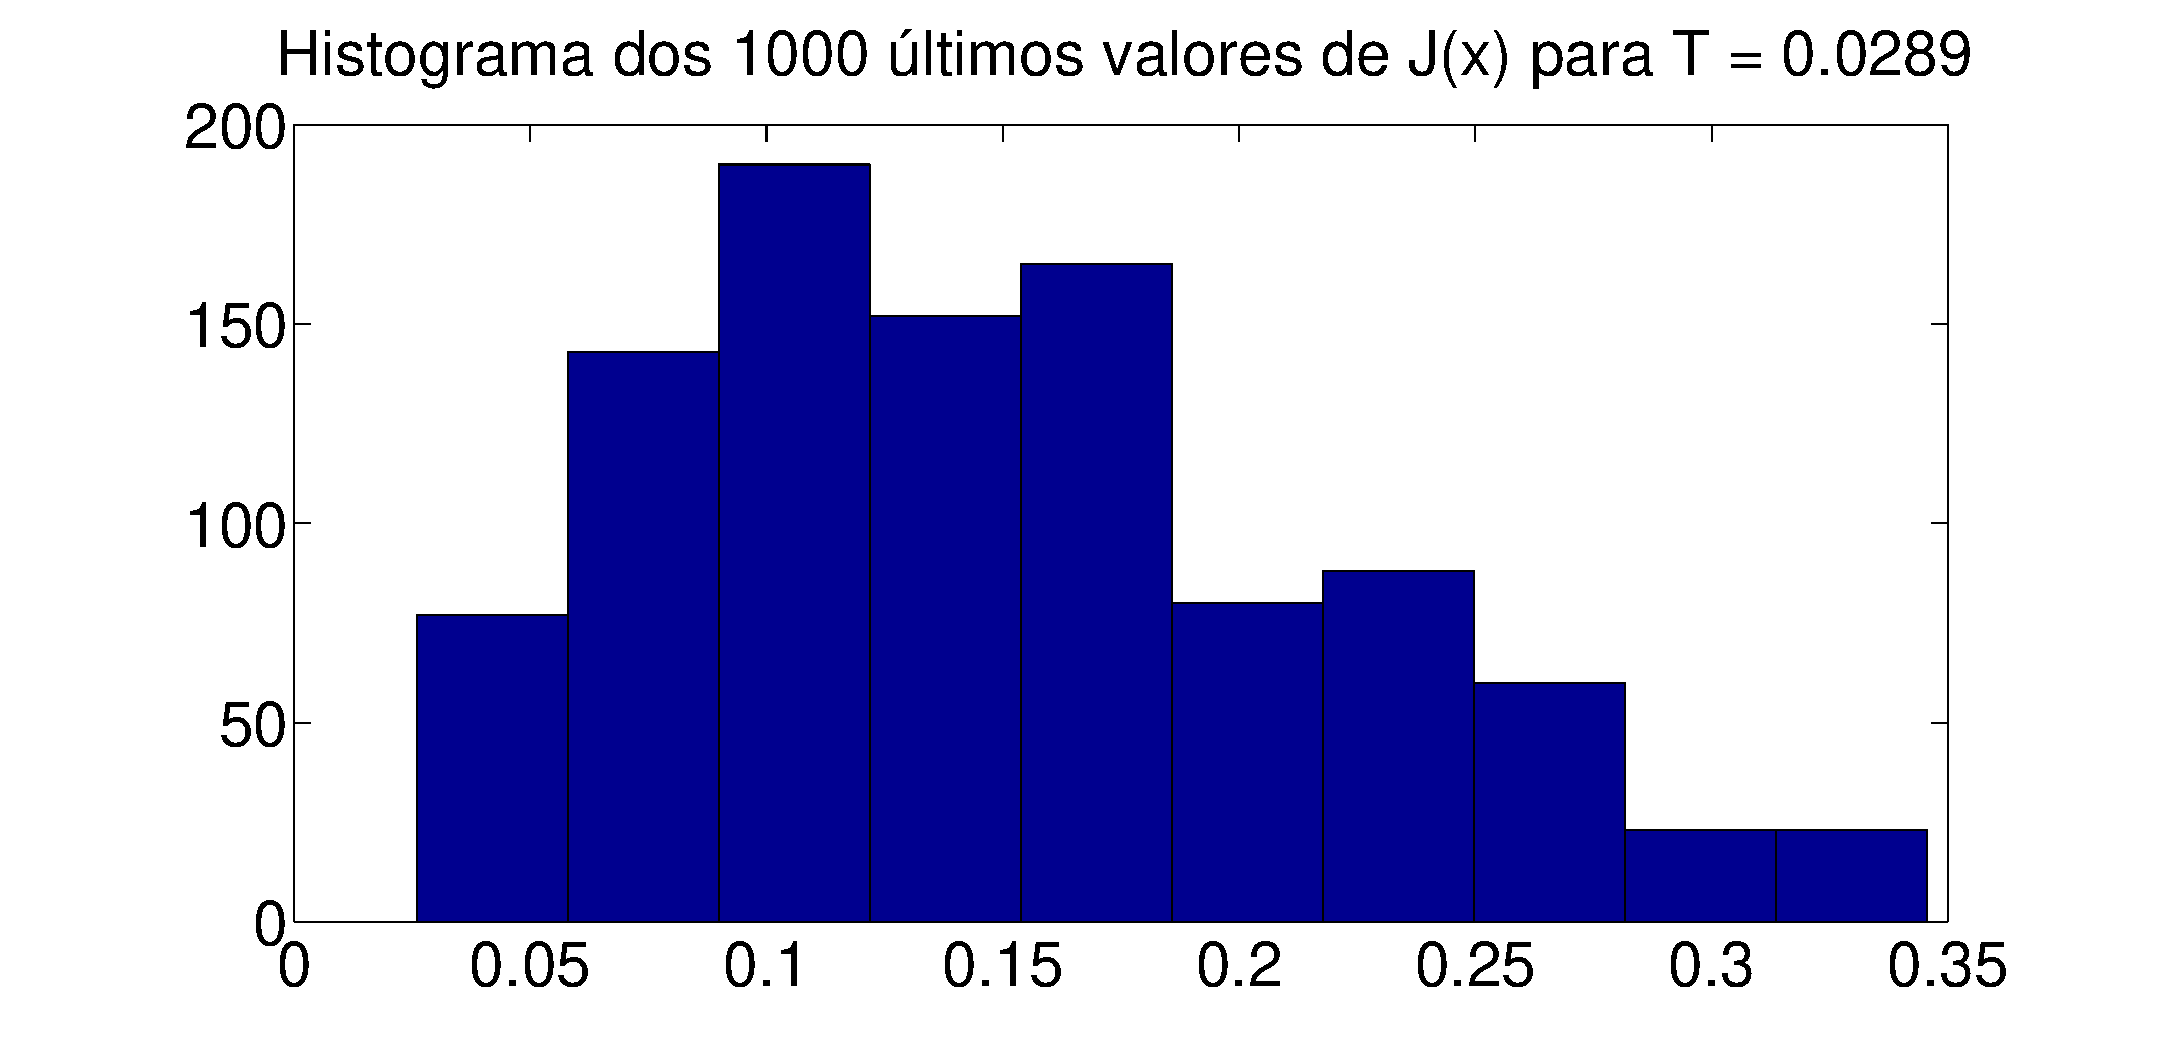
\includegraphics[width = \textwidth]{Q3_histograma_J_t_10}
		\caption{$T = 0.0289$}
	\end{subfigure}
	\begin{subfigure}{0.3\textwidth}
		\centering
		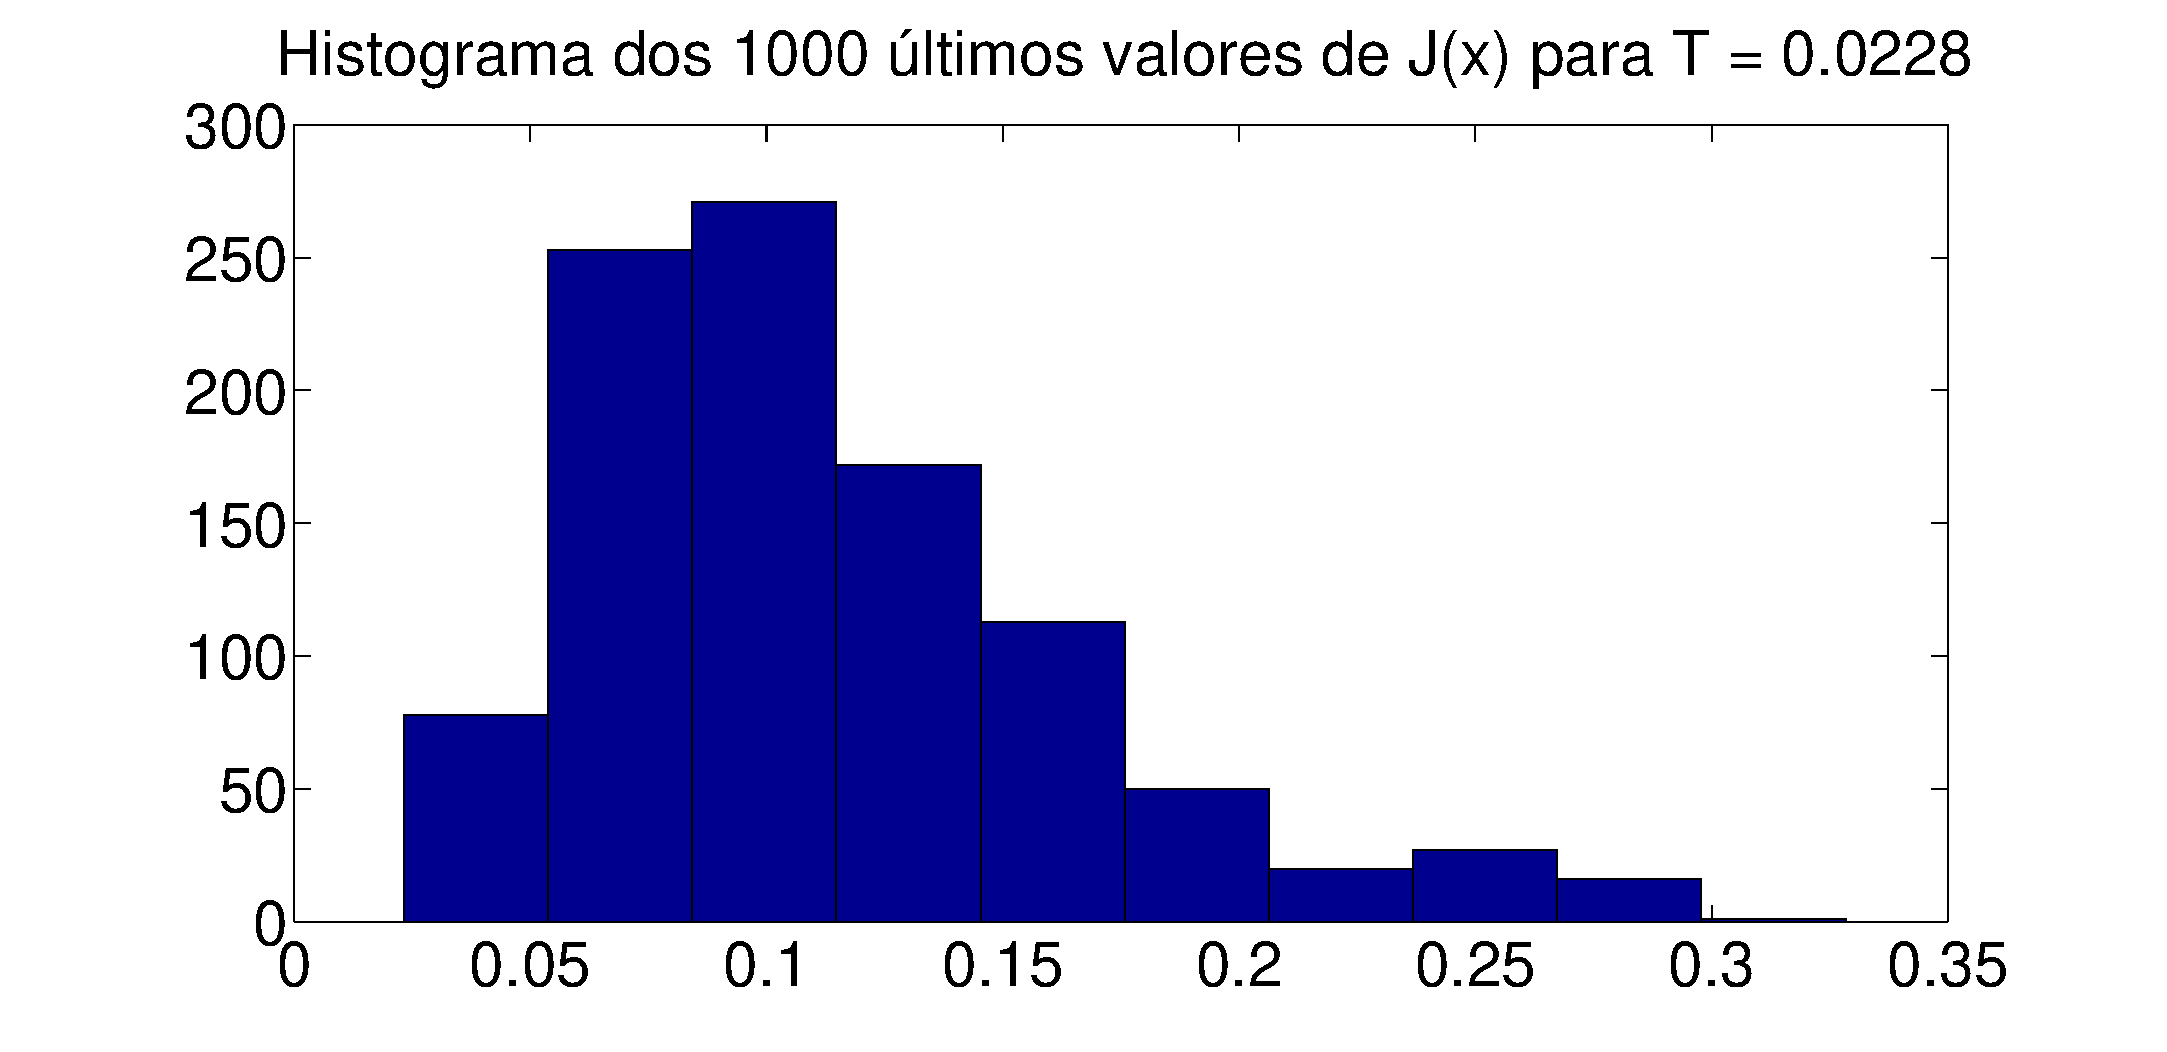
\includegraphics[width = \textwidth]{Q3_histograma_J_t_20}
		\caption{$T = 0.0228$}
	\end{subfigure}
	\caption{Histogramas de valores da função $J(\text{\textbf{x}})$ para diferentes temperaturas.}
	\label{histogramas_custos_temperaturas}
\end{figure}

\end{comment}

\end{document}